\documentclass[twoside]{book}

% Packages required by doxygen
\usepackage{fixltx2e}
\usepackage{calc}
\usepackage{doxygen}
\usepackage{graphicx}
\usepackage[utf8]{inputenc}
\usepackage{makeidx}
\usepackage{multicol}
\usepackage{multirow}
\PassOptionsToPackage{warn}{textcomp}
\usepackage{textcomp}
\usepackage[nointegrals]{wasysym}
\usepackage[table]{xcolor}

% Font selection
\usepackage[T1]{fontenc}
\usepackage{mathptmx}
\usepackage[scaled=.90]{helvet}
\usepackage{courier}
\usepackage{amssymb}
\usepackage{sectsty}
\renewcommand{\familydefault}{\sfdefault}
\allsectionsfont{%
  \fontseries{bc}\selectfont%
  \color{darkgray}%
}
\renewcommand{\DoxyLabelFont}{%
  \fontseries{bc}\selectfont%
  \color{darkgray}%
}
\newcommand{\+}{\discretionary{\mbox{\scriptsize$\hookleftarrow$}}{}{}}

% Page & text layout
\usepackage{geometry}
\geometry{%
  a4paper,%
  top=2.5cm,%
  bottom=2.5cm,%
  left=2.5cm,%
  right=2.5cm%
}
\tolerance=750
\hfuzz=15pt
\hbadness=750
\setlength{\emergencystretch}{15pt}
\setlength{\parindent}{0cm}
\setlength{\parskip}{0.2cm}
\makeatletter
\renewcommand{\paragraph}{%
  \@startsection{paragraph}{4}{0ex}{-1.0ex}{1.0ex}{%
    \normalfont\normalsize\bfseries\SS@parafont%
  }%
}
\renewcommand{\subparagraph}{%
  \@startsection{subparagraph}{5}{0ex}{-1.0ex}{1.0ex}{%
    \normalfont\normalsize\bfseries\SS@subparafont%
  }%
}
\makeatother

% Headers & footers
\usepackage{fancyhdr}
\pagestyle{fancyplain}
\fancyhead[LE]{\fancyplain{}{\bfseries\thepage}}
\fancyhead[CE]{\fancyplain{}{}}
\fancyhead[RE]{\fancyplain{}{\bfseries\leftmark}}
\fancyhead[LO]{\fancyplain{}{\bfseries\rightmark}}
\fancyhead[CO]{\fancyplain{}{}}
\fancyhead[RO]{\fancyplain{}{\bfseries\thepage}}
\fancyfoot[LE]{\fancyplain{}{}}
\fancyfoot[CE]{\fancyplain{}{}}
\fancyfoot[RE]{\fancyplain{}{\bfseries\scriptsize Generated on Wed Aug 9 2017 16\+:09\+:38 for Fastq\+Arazketa by Doxygen }}
\fancyfoot[LO]{\fancyplain{}{\bfseries\scriptsize Generated on Wed Aug 9 2017 16\+:09\+:38 for Fastq\+Arazketa by Doxygen }}
\fancyfoot[CO]{\fancyplain{}{}}
\fancyfoot[RO]{\fancyplain{}{}}
\renewcommand{\footrulewidth}{0.4pt}
\renewcommand{\chaptermark}[1]{%
  \markboth{#1}{}%
}
\renewcommand{\sectionmark}[1]{%
  \markright{\thesection\ #1}%
}

% Indices & bibliography
\usepackage{natbib}
\usepackage[titles]{tocloft}
\setcounter{tocdepth}{3}
\setcounter{secnumdepth}{5}
\makeindex

% Hyperlinks (required, but should be loaded last)
\usepackage{ifpdf}
\ifpdf
  \usepackage[pdftex,pagebackref=true]{hyperref}
\else
  \usepackage[ps2pdf,pagebackref=true]{hyperref}
\fi
\hypersetup{%
  colorlinks=true,%
  linkcolor=blue,%
  citecolor=blue,%
  unicode%
}

% Custom commands
\newcommand{\clearemptydoublepage}{%
  \newpage{\pagestyle{empty}\cleardoublepage}%
}


%===== C O N T E N T S =====

\begin{document}

% Titlepage & ToC
\hypersetup{pageanchor=false,
             bookmarks=true,
             bookmarksnumbered=true,
             pdfencoding=unicode
            }
\pagenumbering{roman}
\begin{titlepage}
\vspace*{7cm}
\begin{center}%
{\Large Fastq\+Arazketa }\\
\vspace*{1cm}
{\large Generated by Doxygen 1.8.8}\\
\vspace*{0.5cm}
{\small Wed Aug 9 2017 16:09:38}\\
\end{center}
\end{titlepage}
\clearemptydoublepage
\tableofcontents
\clearemptydoublepage
\pagenumbering{arabic}
\hypersetup{pageanchor=true}

%--- Begin generated contents ---
\chapter{Class Index}
\section{Class List}
Here are the classes, structs, unions and interfaces with brief descriptions\+:\begin{DoxyCompactList}
\item\contentsline{section}{\hyperlink{struct__adapter}{\+\_\+adapter} }{\pageref{struct__adapter}}{}
\item\contentsline{section}{\hyperlink{struct__fa__data}{\+\_\+fa\+\_\+data} \\*Stores sequences of a fasta file }{\pageref{struct__fa__data}}{}
\item\contentsline{section}{\hyperlink{struct__fa__entry}{\+\_\+fa\+\_\+entry} \\*Fasta entry }{\pageref{struct__fa__entry}}{}
\item\contentsline{section}{\hyperlink{struct__fq__read}{\+\_\+fq\+\_\+read} \\*Stores a fastq entry }{\pageref{struct__fq__read}}{}
\item\contentsline{section}{\hyperlink{struct__iparam__Freport}{\+\_\+iparam\+\_\+\+Freport} \\*Freport input parameters }{\pageref{struct__iparam__Freport}}{}
\item\contentsline{section}{\hyperlink{struct__iparam__makeTree}{\+\_\+iparam\+\_\+make\+Tree} \\*Make\+Tree input parameters }{\pageref{struct__iparam__makeTree}}{}
\item\contentsline{section}{\hyperlink{struct__iparam__Qreport}{\+\_\+iparam\+\_\+\+Qreport} \\*Qreport input parameters }{\pageref{struct__iparam__Qreport}}{}
\item\contentsline{section}{\hyperlink{struct__iparam__Sreport}{\+\_\+iparam\+\_\+\+Sreport} \\*Sreport input parameters }{\pageref{struct__iparam__Sreport}}{}
\item\contentsline{section}{\hyperlink{struct__iparam__trimFilter}{\+\_\+iparam\+\_\+trim\+Filter} \\*Trim\+Filter input parameters }{\pageref{struct__iparam__trimFilter}}{}
\item\contentsline{section}{\hyperlink{struct__node}{\+\_\+node} \\*Node structure\+: formed out of T\+\_\+\+A\+C\+G\+T pointers to Node structure }{\pageref{struct__node}}{}
\item\contentsline{section}{\hyperlink{struct__split}{\+\_\+split} \\*Splitted string and the number or splitted fields }{\pageref{struct__split}}{}
\item\contentsline{section}{\hyperlink{struct__stats__TF}{\+\_\+stats\+\_\+\+T\+F} \\*Collects stats info from the filtering procedure }{\pageref{struct__stats__TF}}{}
\item\contentsline{section}{\hyperlink{struct__tree}{\+\_\+tree} \\*Structure containing a T\+\_\+\+A\+C\+G\+T-\/tree }{\pageref{struct__tree}}{}
\item\contentsline{section}{\hyperlink{structstatsinfo}{statsinfo} \\*Stores info needed to create the summary graphs }{\pageref{structstatsinfo}}{}
\end{DoxyCompactList}

\chapter{File Index}
\section{File List}
Here is a list of all documented files with brief descriptions\+:\begin{DoxyCompactList}
\item\contentsline{section}{include/\hyperlink{defines_8h}{defines.\+h} \\*Macro definitions }{\pageref{defines_8h}}{}
\item\contentsline{section}{include/\hyperlink{fa__read_8h}{fa\+\_\+read.\+h} \\*Reads in and stores fasta files }{\pageref{fa__read_8h}}{}
\item\contentsline{section}{include/\hyperlink{fopen__gen_8h}{fopen\+\_\+gen.\+h} \\*Uncompress/compress input/output files using pipes }{\pageref{fopen__gen_8h}}{}
\item\contentsline{section}{include/\hyperlink{fq__read_8h}{fq\+\_\+read.\+h} \\*Fastq entries manipulations (read/write) }{\pageref{fq__read_8h}}{}
\item\contentsline{section}{include/\hyperlink{init__Qreport_8h}{init\+\_\+\+Qreport.\+h} \\*Header file\+: help dialog for Qreport and initialization of the command line arguments }{\pageref{init__Qreport_8h}}{}
\item\contentsline{section}{include/\hyperlink{init__Sreport_8h}{init\+\_\+\+Sreport.\+h} \\*Help dialog for Sreport and initialization of the command line arguments }{\pageref{init__Sreport_8h}}{}
\item\contentsline{section}{include/\hyperlink{Lmer_8h}{Lmer.\+h} \\*Manipulation of Lmers and sequences }{\pageref{Lmer_8h}}{}
\item\contentsline{section}{include/\hyperlink{Rcommand__Qreport_8h}{Rcommand\+\_\+\+Qreport.\+h} \\*Get Rscript command for Qreport }{\pageref{Rcommand__Qreport_8h}}{}
\item\contentsline{section}{include/\hyperlink{Rcommand__Sreport_8h}{Rcommand\+\_\+\+Sreport.\+h} \\*Get Rscript command for Sreport }{\pageref{Rcommand__Sreport_8h}}{}
\item\contentsline{section}{include/\hyperlink{stats__info_8h}{stats\+\_\+info.\+h} \\*Construct the quality report variables and update them }{\pageref{stats__info_8h}}{}
\item\contentsline{section}{include/\hyperlink{str__manip_8h}{str\+\_\+manip.\+h} \\*Functions that do string manipulation }{\pageref{str__manip_8h}}{}
\item\contentsline{section}{src/\hyperlink{fa__read_8c}{fa\+\_\+read.\+c} \\*Reads in and stores fasta files }{\pageref{fa__read_8c}}{}
\item\contentsline{section}{src/\hyperlink{fopen__gen_8c}{fopen\+\_\+gen.\+c} \\*Uncompress/compress input/output files using pipes }{\pageref{fopen__gen_8c}}{}
\item\contentsline{section}{src/\hyperlink{fq__read_8c}{fq\+\_\+read.\+c} \\*Fastq entries manipulations (read/write) }{\pageref{fq__read_8c}}{}
\item\contentsline{section}{src/\hyperlink{init__Qreport_8c}{init\+\_\+\+Qreport.\+c} \\*Help dialog for Qreport and initialization of the command line arguments }{\pageref{init__Qreport_8c}}{}
\item\contentsline{section}{src/\hyperlink{init__Sreport_8c}{init\+\_\+\+Sreport.\+c} \\*Help dialog for Sreport and initialization of the command line arguments }{\pageref{init__Sreport_8c}}{}
\item\contentsline{section}{src/\hyperlink{Lmer_8c}{Lmer.\+c} \\*Manipulation of Lmers and sequences }{\pageref{Lmer_8c}}{}
\item\contentsline{section}{src/\hyperlink{Qreport_8c}{Qreport.\+c} \\*Q\+Report main function }{\pageref{Qreport_8c}}{}
\item\contentsline{section}{src/\hyperlink{Rcommand__Sreport_8c}{Rcommand\+\_\+\+Sreport.\+c} \\*Get Rscript command for Sreport }{\pageref{Rcommand__Sreport_8c}}{}
\item\contentsline{section}{src/\hyperlink{Sreport_8c}{Sreport.\+c} \\*Sreport main function }{\pageref{Sreport_8c}}{}
\item\contentsline{section}{src/\hyperlink{stats__info_8c}{stats\+\_\+info.\+c} \\*Construct the quality report variables and update them }{\pageref{stats__info_8c}}{}
\item\contentsline{section}{src/\hyperlink{str__manip_8c}{str\+\_\+manip.\+c} \\*Functions that do string manipulation }{\pageref{str__manip_8c}}{}
\end{DoxyCompactList}

\chapter{Class Documentation}
\hypertarget{struct__fq__read}{}\section{\+\_\+fq\+\_\+read Struct Reference}
\label{struct__fq__read}\index{\+\_\+fq\+\_\+read@{\+\_\+fq\+\_\+read}}


stores a fastq entry  




{\ttfamily \#include $<$fq\+\_\+read.\+h$>$}

\subsection*{Public Attributes}
\begin{DoxyCompactItemize}
\item 
char \mbox{\hyperlink{struct__fq__read_a7a643c49516b3a35f221d0fcda7f9ff3}{line1}} \mbox{[}R\+E\+A\+D\+\_\+\+M\+A\+X\+L\+EN\mbox{]}
\item 
char \mbox{\hyperlink{struct__fq__read_af2502a6f97e9508936c1b9f08890cc84}{line2}} \mbox{[}R\+E\+A\+D\+\_\+\+M\+A\+X\+L\+EN\mbox{]}
\item 
char \mbox{\hyperlink{struct__fq__read_a3df48e8dc31e47dc36c371002dba1bb5}{line3}} \mbox{[}R\+E\+A\+D\+\_\+\+M\+A\+X\+L\+EN\mbox{]}
\item 
char \mbox{\hyperlink{struct__fq__read_a8074fd734cb7e3d4b87454417aea569a}{line4}} \mbox{[}R\+E\+A\+D\+\_\+\+M\+A\+X\+L\+EN\mbox{]}
\item 
int \mbox{\hyperlink{struct__fq__read_a746efa9093b5223e85ffb7274e7693ef}{L}}
\item 
int \mbox{\hyperlink{struct__fq__read_a0b8deb6c25c72026b4928b17e3f12ade}{start}}
\item 
int \mbox{\hyperlink{struct__fq__read_a9cf08b81f1e78553e08fb597d30192b6}{Lhalf}}
\item 
char \mbox{\hyperlink{struct__fq__read_aae3ecb937cbba51f91baa391d8d84826}{extended}} \mbox{[}R\+E\+A\+D\+\_\+\+M\+A\+X\+L\+EN\mbox{]}
\item 
unsigned char \mbox{\hyperlink{struct__fq__read_afd023930012710b1a015ef78a02b3721}{pack}} \mbox{[}(R\+E\+A\+D\+\_\+\+M\+A\+X\+L\+EN+1)/2\mbox{]}
\item 
unsigned char \mbox{\hyperlink{struct__fq__read_a8c9786c5779078561abe5ec2e06c7ff9}{packsh}} \mbox{[}(R\+E\+A\+D\+\_\+\+M\+A\+X\+L\+EN+1)/2\mbox{]}
\item 
int \mbox{\hyperlink{struct__fq__read_a61c338fcae059e8581b02ec1b2cdcdc6}{L\+\_\+ad}}
\item 
int \mbox{\hyperlink{struct__fq__read_acf9a80768c42f71a975d602058e2ab52}{L\+\_\+ext}}
\item 
int \mbox{\hyperlink{struct__fq__read_a84f64405e7a9bbc055dd4f5534041782}{L\+\_\+pack}}
\item 
int \mbox{\hyperlink{struct__fq__read_a1303e633bdb4a7e31083d849a92fcbcc}{L\+\_\+packsh}}
\end{DoxyCompactItemize}


\subsection{Detailed Description}
stores a fastq entry 

\subsection{Member Data Documentation}
\mbox{\Hypertarget{struct__fq__read_aae3ecb937cbba51f91baa391d8d84826}\label{struct__fq__read_aae3ecb937cbba51f91baa391d8d84826}} 
\index{\+\_\+fq\+\_\+read@{\+\_\+fq\+\_\+read}!extended@{extended}}
\index{extended@{extended}!\+\_\+fq\+\_\+read@{\+\_\+fq\+\_\+read}}
\subsubsection{\texorpdfstring{extended}{extended}}
{\footnotesize\ttfamily char \+\_\+fq\+\_\+read\+::extended\mbox{[}R\+E\+A\+D\+\_\+\+M\+A\+X\+L\+EN\mbox{]}}

extended sequence, adapter added to 5\textquotesingle{} end \mbox{\Hypertarget{struct__fq__read_a746efa9093b5223e85ffb7274e7693ef}\label{struct__fq__read_a746efa9093b5223e85ffb7274e7693ef}} 
\index{\+\_\+fq\+\_\+read@{\+\_\+fq\+\_\+read}!L@{L}}
\index{L@{L}!\+\_\+fq\+\_\+read@{\+\_\+fq\+\_\+read}}
\subsubsection{\texorpdfstring{L}{L}}
{\footnotesize\ttfamily int \+\_\+fq\+\_\+read\+::L}

read length \mbox{\Hypertarget{struct__fq__read_a61c338fcae059e8581b02ec1b2cdcdc6}\label{struct__fq__read_a61c338fcae059e8581b02ec1b2cdcdc6}} 
\index{\+\_\+fq\+\_\+read@{\+\_\+fq\+\_\+read}!L\+\_\+ad@{L\+\_\+ad}}
\index{L\+\_\+ad@{L\+\_\+ad}!\+\_\+fq\+\_\+read@{\+\_\+fq\+\_\+read}}
\subsubsection{\texorpdfstring{L\+\_\+ad}{L\_ad}}
{\footnotesize\ttfamily int \+\_\+fq\+\_\+read\+::\+L\+\_\+ad}

length of adapter sequence \mbox{\Hypertarget{struct__fq__read_acf9a80768c42f71a975d602058e2ab52}\label{struct__fq__read_acf9a80768c42f71a975d602058e2ab52}} 
\index{\+\_\+fq\+\_\+read@{\+\_\+fq\+\_\+read}!L\+\_\+ext@{L\+\_\+ext}}
\index{L\+\_\+ext@{L\+\_\+ext}!\+\_\+fq\+\_\+read@{\+\_\+fq\+\_\+read}}
\subsubsection{\texorpdfstring{L\+\_\+ext}{L\_ext}}
{\footnotesize\ttfamily int \+\_\+fq\+\_\+read\+::\+L\+\_\+ext}

length of extended sequence \mbox{\Hypertarget{struct__fq__read_a84f64405e7a9bbc055dd4f5534041782}\label{struct__fq__read_a84f64405e7a9bbc055dd4f5534041782}} 
\index{\+\_\+fq\+\_\+read@{\+\_\+fq\+\_\+read}!L\+\_\+pack@{L\+\_\+pack}}
\index{L\+\_\+pack@{L\+\_\+pack}!\+\_\+fq\+\_\+read@{\+\_\+fq\+\_\+read}}
\subsubsection{\texorpdfstring{L\+\_\+pack}{L\_pack}}
{\footnotesize\ttfamily int \+\_\+fq\+\_\+read\+::\+L\+\_\+pack}

length of packed sequence \mbox{\Hypertarget{struct__fq__read_a1303e633bdb4a7e31083d849a92fcbcc}\label{struct__fq__read_a1303e633bdb4a7e31083d849a92fcbcc}} 
\index{\+\_\+fq\+\_\+read@{\+\_\+fq\+\_\+read}!L\+\_\+packsh@{L\+\_\+packsh}}
\index{L\+\_\+packsh@{L\+\_\+packsh}!\+\_\+fq\+\_\+read@{\+\_\+fq\+\_\+read}}
\subsubsection{\texorpdfstring{L\+\_\+packsh}{L\_packsh}}
{\footnotesize\ttfamily int \+\_\+fq\+\_\+read\+::\+L\+\_\+packsh}

length of packed sequence (shifted) \mbox{\Hypertarget{struct__fq__read_a9cf08b81f1e78553e08fb597d30192b6}\label{struct__fq__read_a9cf08b81f1e78553e08fb597d30192b6}} 
\index{\+\_\+fq\+\_\+read@{\+\_\+fq\+\_\+read}!Lhalf@{Lhalf}}
\index{Lhalf@{Lhalf}!\+\_\+fq\+\_\+read@{\+\_\+fq\+\_\+read}}
\subsubsection{\texorpdfstring{Lhalf}{Lhalf}}
{\footnotesize\ttfamily int \+\_\+fq\+\_\+read\+::\+Lhalf}

half of read length \mbox{\Hypertarget{struct__fq__read_a7a643c49516b3a35f221d0fcda7f9ff3}\label{struct__fq__read_a7a643c49516b3a35f221d0fcda7f9ff3}} 
\index{\+\_\+fq\+\_\+read@{\+\_\+fq\+\_\+read}!line1@{line1}}
\index{line1@{line1}!\+\_\+fq\+\_\+read@{\+\_\+fq\+\_\+read}}
\subsubsection{\texorpdfstring{line1}{line1}}
{\footnotesize\ttfamily char \+\_\+fq\+\_\+read\+::line1\mbox{[}R\+E\+A\+D\+\_\+\+M\+A\+X\+L\+EN\mbox{]}}

Line 1 in fastq entry \mbox{\Hypertarget{struct__fq__read_af2502a6f97e9508936c1b9f08890cc84}\label{struct__fq__read_af2502a6f97e9508936c1b9f08890cc84}} 
\index{\+\_\+fq\+\_\+read@{\+\_\+fq\+\_\+read}!line2@{line2}}
\index{line2@{line2}!\+\_\+fq\+\_\+read@{\+\_\+fq\+\_\+read}}
\subsubsection{\texorpdfstring{line2}{line2}}
{\footnotesize\ttfamily char \+\_\+fq\+\_\+read\+::line2\mbox{[}R\+E\+A\+D\+\_\+\+M\+A\+X\+L\+EN\mbox{]}}

Line 2 in fastq entry \mbox{\Hypertarget{struct__fq__read_a3df48e8dc31e47dc36c371002dba1bb5}\label{struct__fq__read_a3df48e8dc31e47dc36c371002dba1bb5}} 
\index{\+\_\+fq\+\_\+read@{\+\_\+fq\+\_\+read}!line3@{line3}}
\index{line3@{line3}!\+\_\+fq\+\_\+read@{\+\_\+fq\+\_\+read}}
\subsubsection{\texorpdfstring{line3}{line3}}
{\footnotesize\ttfamily char \+\_\+fq\+\_\+read\+::line3\mbox{[}R\+E\+A\+D\+\_\+\+M\+A\+X\+L\+EN\mbox{]}}

Line 3 in fastq entry \mbox{\Hypertarget{struct__fq__read_a8074fd734cb7e3d4b87454417aea569a}\label{struct__fq__read_a8074fd734cb7e3d4b87454417aea569a}} 
\index{\+\_\+fq\+\_\+read@{\+\_\+fq\+\_\+read}!line4@{line4}}
\index{line4@{line4}!\+\_\+fq\+\_\+read@{\+\_\+fq\+\_\+read}}
\subsubsection{\texorpdfstring{line4}{line4}}
{\footnotesize\ttfamily char \+\_\+fq\+\_\+read\+::line4\mbox{[}R\+E\+A\+D\+\_\+\+M\+A\+X\+L\+EN\mbox{]}}

Line 4 in fastq entry \mbox{\Hypertarget{struct__fq__read_afd023930012710b1a015ef78a02b3721}\label{struct__fq__read_afd023930012710b1a015ef78a02b3721}} 
\index{\+\_\+fq\+\_\+read@{\+\_\+fq\+\_\+read}!pack@{pack}}
\index{pack@{pack}!\+\_\+fq\+\_\+read@{\+\_\+fq\+\_\+read}}
\subsubsection{\texorpdfstring{pack}{pack}}
{\footnotesize\ttfamily unsigned char \+\_\+fq\+\_\+read\+::pack\mbox{[}(R\+E\+A\+D\+\_\+\+M\+A\+X\+L\+EN+1)/2\mbox{]}}

pack sequence \mbox{\Hypertarget{struct__fq__read_a8c9786c5779078561abe5ec2e06c7ff9}\label{struct__fq__read_a8c9786c5779078561abe5ec2e06c7ff9}} 
\index{\+\_\+fq\+\_\+read@{\+\_\+fq\+\_\+read}!packsh@{packsh}}
\index{packsh@{packsh}!\+\_\+fq\+\_\+read@{\+\_\+fq\+\_\+read}}
\subsubsection{\texorpdfstring{packsh}{packsh}}
{\footnotesize\ttfamily unsigned char \+\_\+fq\+\_\+read\+::packsh\mbox{[}(R\+E\+A\+D\+\_\+\+M\+A\+X\+L\+EN+1)/2\mbox{]}}

pack sequence with shift \mbox{\Hypertarget{struct__fq__read_a0b8deb6c25c72026b4928b17e3f12ade}\label{struct__fq__read_a0b8deb6c25c72026b4928b17e3f12ade}} 
\index{\+\_\+fq\+\_\+read@{\+\_\+fq\+\_\+read}!start@{start}}
\index{start@{start}!\+\_\+fq\+\_\+read@{\+\_\+fq\+\_\+read}}
\subsubsection{\texorpdfstring{start}{start}}
{\footnotesize\ttfamily int \+\_\+fq\+\_\+read\+::start}

nucleotide position start. Can only be different from zero if the read has been filtered with this tool. 

The documentation for this struct was generated from the following file\+:\begin{DoxyCompactItemize}
\item 
include/\mbox{\hyperlink{fq__read_8h}{fq\+\_\+read.\+h}}\end{DoxyCompactItemize}

\hypertarget{struct__iparam__Qreport}{\section{\+\_\+iparam\+\_\+\+Qreport Struct Reference}
\label{struct__iparam__Qreport}\index{\+\_\+iparam\+\_\+\+Qreport@{\+\_\+iparam\+\_\+\+Qreport}}
}


contains Qreport input parameters  




{\ttfamily \#include $<$init\+\_\+\+Qreport.\+h$>$}

\subsection*{Public Attributes}
\begin{DoxyCompactItemize}
\item 
char $\ast$ \hyperlink{struct__iparam__Qreport_ac96f6463d81dc1fcc41850564f24cf11}{inputfile}
\item 
char \hyperlink{struct__iparam__Qreport_abdf92f14bc1c49787cda4b94ceb668cd}{outputfilebin} \mbox{[}\hyperlink{defines_8h_abe0ec333b60117063f9b9fd9f849cb08}{M\+A\+X\+\_\+\+F\+I\+L\+E\+N\+A\+M\+E}\mbox{]}
\item 
char \hyperlink{struct__iparam__Qreport_a54ffbb27584db445494af7d9a1c214de}{outputfilehtml} \mbox{[}\hyperlink{defines_8h_abe0ec333b60117063f9b9fd9f849cb08}{M\+A\+X\+\_\+\+F\+I\+L\+E\+N\+A\+M\+E}\mbox{]}
\item 
char \hyperlink{struct__iparam__Qreport_a75f5c38f9365c0c1370040928f43d316}{outputfileinfo} \mbox{[}\hyperlink{defines_8h_abe0ec333b60117063f9b9fd9f849cb08}{M\+A\+X\+\_\+\+F\+I\+L\+E\+N\+A\+M\+E}\mbox{]}
\item 
int \hyperlink{struct__iparam__Qreport_a47cfa018e6e957cb132e22876a400a1f}{n\+Q}
\item 
int \hyperlink{struct__iparam__Qreport_a9d91db490f318f69dcea4999f630712e}{ntiles}
\item 
int \hyperlink{struct__iparam__Qreport_a1fa54b38e988ffe30eba5e0284e9dacb}{min\+Q}
\item 
int \hyperlink{struct__iparam__Qreport_a1004bab2a5776669710b74925ba4d338}{read\+\_\+len}
\item 
int \hyperlink{struct__iparam__Qreport_ae1ce417a16c5d30c05a09ec868154e14}{filter}
\item 
int \hyperlink{struct__iparam__Qreport_a0a09c5cc791e625b948acb45b39164e6}{one\+\_\+read\+\_\+len}
\end{DoxyCompactItemize}


\subsection{Detailed Description}
contains Qreport input parameters 

\subsection{Member Data Documentation}
\hypertarget{struct__iparam__Qreport_ae1ce417a16c5d30c05a09ec868154e14}{\index{\+\_\+iparam\+\_\+\+Qreport@{\+\_\+iparam\+\_\+\+Qreport}!filter@{filter}}
\index{filter@{filter}!\+\_\+iparam\+\_\+\+Qreport@{\+\_\+iparam\+\_\+\+Qreport}}
\subsubsection[{filter}]{\setlength{\rightskip}{0pt plus 5cm}int \+\_\+iparam\+\_\+\+Qreport\+::filter}}\label{struct__iparam__Qreport_ae1ce417a16c5d30c05a09ec868154e14}
0 original data, 1 this tool filtered data, 2 other tool filtered data \hypertarget{struct__iparam__Qreport_ac96f6463d81dc1fcc41850564f24cf11}{\index{\+\_\+iparam\+\_\+\+Qreport@{\+\_\+iparam\+\_\+\+Qreport}!inputfile@{inputfile}}
\index{inputfile@{inputfile}!\+\_\+iparam\+\_\+\+Qreport@{\+\_\+iparam\+\_\+\+Qreport}}
\subsubsection[{inputfile}]{\setlength{\rightskip}{0pt plus 5cm}char$\ast$ \+\_\+iparam\+\_\+\+Qreport\+::inputfile}}\label{struct__iparam__Qreport_ac96f6463d81dc1fcc41850564f24cf11}
Inputfile name \hypertarget{struct__iparam__Qreport_a1fa54b38e988ffe30eba5e0284e9dacb}{\index{\+\_\+iparam\+\_\+\+Qreport@{\+\_\+iparam\+\_\+\+Qreport}!min\+Q@{min\+Q}}
\index{min\+Q@{min\+Q}!\+\_\+iparam\+\_\+\+Qreport@{\+\_\+iparam\+\_\+\+Qreport}}
\subsubsection[{min\+Q}]{\setlength{\rightskip}{0pt plus 5cm}int \+\_\+iparam\+\_\+\+Qreport\+::min\+Q}}\label{struct__iparam__Qreport_a1fa54b38e988ffe30eba5e0284e9dacb}
minimum Quality allowed 0 -\/ 45 \hypertarget{struct__iparam__Qreport_a47cfa018e6e957cb132e22876a400a1f}{\index{\+\_\+iparam\+\_\+\+Qreport@{\+\_\+iparam\+\_\+\+Qreport}!n\+Q@{n\+Q}}
\index{n\+Q@{n\+Q}!\+\_\+iparam\+\_\+\+Qreport@{\+\_\+iparam\+\_\+\+Qreport}}
\subsubsection[{n\+Q}]{\setlength{\rightskip}{0pt plus 5cm}int \+\_\+iparam\+\_\+\+Qreport\+::n\+Q}}\label{struct__iparam__Qreport_a47cfa018e6e957cb132e22876a400a1f}
\# different quality values (default is 46) \hypertarget{struct__iparam__Qreport_a9d91db490f318f69dcea4999f630712e}{\index{\+\_\+iparam\+\_\+\+Qreport@{\+\_\+iparam\+\_\+\+Qreport}!ntiles@{ntiles}}
\index{ntiles@{ntiles}!\+\_\+iparam\+\_\+\+Qreport@{\+\_\+iparam\+\_\+\+Qreport}}
\subsubsection[{ntiles}]{\setlength{\rightskip}{0pt plus 5cm}int \+\_\+iparam\+\_\+\+Qreport\+::ntiles}}\label{struct__iparam__Qreport_a9d91db490f318f69dcea4999f630712e}
\# tiles (default is 96) \hypertarget{struct__iparam__Qreport_a0a09c5cc791e625b948acb45b39164e6}{\index{\+\_\+iparam\+\_\+\+Qreport@{\+\_\+iparam\+\_\+\+Qreport}!one\+\_\+read\+\_\+len@{one\+\_\+read\+\_\+len}}
\index{one\+\_\+read\+\_\+len@{one\+\_\+read\+\_\+len}!\+\_\+iparam\+\_\+\+Qreport@{\+\_\+iparam\+\_\+\+Qreport}}
\subsubsection[{one\+\_\+read\+\_\+len}]{\setlength{\rightskip}{0pt plus 5cm}int \+\_\+iparam\+\_\+\+Qreport\+::one\+\_\+read\+\_\+len}}\label{struct__iparam__Qreport_a0a09c5cc791e625b948acb45b39164e6}
1 all reads of equal length 0 reads have different lengths. \hypertarget{struct__iparam__Qreport_abdf92f14bc1c49787cda4b94ceb668cd}{\index{\+\_\+iparam\+\_\+\+Qreport@{\+\_\+iparam\+\_\+\+Qreport}!outputfilebin@{outputfilebin}}
\index{outputfilebin@{outputfilebin}!\+\_\+iparam\+\_\+\+Qreport@{\+\_\+iparam\+\_\+\+Qreport}}
\subsubsection[{outputfilebin}]{\setlength{\rightskip}{0pt plus 5cm}char \+\_\+iparam\+\_\+\+Qreport\+::outputfilebin\mbox{[}{\bf M\+A\+X\+\_\+\+F\+I\+L\+E\+N\+A\+M\+E}\mbox{]}}}\label{struct__iparam__Qreport_abdf92f14bc1c49787cda4b94ceb668cd}
Binary outputfile name. \hypertarget{struct__iparam__Qreport_a54ffbb27584db445494af7d9a1c214de}{\index{\+\_\+iparam\+\_\+\+Qreport@{\+\_\+iparam\+\_\+\+Qreport}!outputfilehtml@{outputfilehtml}}
\index{outputfilehtml@{outputfilehtml}!\+\_\+iparam\+\_\+\+Qreport@{\+\_\+iparam\+\_\+\+Qreport}}
\subsubsection[{outputfilehtml}]{\setlength{\rightskip}{0pt plus 5cm}char \+\_\+iparam\+\_\+\+Qreport\+::outputfilehtml\mbox{[}{\bf M\+A\+X\+\_\+\+F\+I\+L\+E\+N\+A\+M\+E}\mbox{]}}}\label{struct__iparam__Qreport_a54ffbb27584db445494af7d9a1c214de}
html outputfile name \hypertarget{struct__iparam__Qreport_a75f5c38f9365c0c1370040928f43d316}{\index{\+\_\+iparam\+\_\+\+Qreport@{\+\_\+iparam\+\_\+\+Qreport}!outputfileinfo@{outputfileinfo}}
\index{outputfileinfo@{outputfileinfo}!\+\_\+iparam\+\_\+\+Qreport@{\+\_\+iparam\+\_\+\+Qreport}}
\subsubsection[{outputfileinfo}]{\setlength{\rightskip}{0pt plus 5cm}char \+\_\+iparam\+\_\+\+Qreport\+::outputfileinfo\mbox{[}{\bf M\+A\+X\+\_\+\+F\+I\+L\+E\+N\+A\+M\+E}\mbox{]}}}\label{struct__iparam__Qreport_a75f5c38f9365c0c1370040928f43d316}
Info outputfile name \hypertarget{struct__iparam__Qreport_a1004bab2a5776669710b74925ba4d338}{\index{\+\_\+iparam\+\_\+\+Qreport@{\+\_\+iparam\+\_\+\+Qreport}!read\+\_\+len@{read\+\_\+len}}
\index{read\+\_\+len@{read\+\_\+len}!\+\_\+iparam\+\_\+\+Qreport@{\+\_\+iparam\+\_\+\+Qreport}}
\subsubsection[{read\+\_\+len}]{\setlength{\rightskip}{0pt plus 5cm}int \+\_\+iparam\+\_\+\+Qreport\+::read\+\_\+len}}\label{struct__iparam__Qreport_a1004bab2a5776669710b74925ba4d338}
original read length 

The documentation for this struct was generated from the following file\+:\begin{DoxyCompactItemize}
\item 
include/\hyperlink{init__Qreport_8h}{init\+\_\+\+Qreport.\+h}\end{DoxyCompactItemize}

\hypertarget{struct__iparam__Sreport}{\section{\+\_\+iparam\+\_\+\+Sreport Struct Reference}
\label{struct__iparam__Sreport}\index{\+\_\+iparam\+\_\+\+Sreport@{\+\_\+iparam\+\_\+\+Sreport}}
}


contains Sreport input parameters  




{\ttfamily \#include $<$init\+\_\+\+Sreport.\+h$>$}

\subsection*{Public Attributes}
\begin{DoxyCompactItemize}
\item 
char $\ast$ \hyperlink{struct__iparam__Sreport_af5521a185f440566547b4b11b9fac6a4}{inputfolder}
\item 
char \hyperlink{struct__iparam__Sreport_aab71d9b5647daf65a8ba9ba6f7a35ee5}{outputfile} \mbox{[}\hyperlink{defines_8h_abe0ec333b60117063f9b9fd9f849cb08}{M\+A\+X\+\_\+\+F\+I\+L\+E\+N\+A\+M\+E}\mbox{]}
\end{DoxyCompactItemize}


\subsection{Detailed Description}
contains Sreport input parameters 

\subsection{Member Data Documentation}
\hypertarget{struct__iparam__Sreport_af5521a185f440566547b4b11b9fac6a4}{\index{\+\_\+iparam\+\_\+\+Sreport@{\+\_\+iparam\+\_\+\+Sreport}!inputfolder@{inputfolder}}
\index{inputfolder@{inputfolder}!\+\_\+iparam\+\_\+\+Sreport@{\+\_\+iparam\+\_\+\+Sreport}}
\subsubsection[{inputfolder}]{\setlength{\rightskip}{0pt plus 5cm}char$\ast$ \+\_\+iparam\+\_\+\+Sreport\+::inputfolder}}\label{struct__iparam__Sreport_af5521a185f440566547b4b11b9fac6a4}
input folder \hypertarget{struct__iparam__Sreport_aab71d9b5647daf65a8ba9ba6f7a35ee5}{\index{\+\_\+iparam\+\_\+\+Sreport@{\+\_\+iparam\+\_\+\+Sreport}!outputfile@{outputfile}}
\index{outputfile@{outputfile}!\+\_\+iparam\+\_\+\+Sreport@{\+\_\+iparam\+\_\+\+Sreport}}
\subsubsection[{outputfile}]{\setlength{\rightskip}{0pt plus 5cm}char \+\_\+iparam\+\_\+\+Sreport\+::outputfile\mbox{[}{\bf M\+A\+X\+\_\+\+F\+I\+L\+E\+N\+A\+M\+E}\mbox{]}}}\label{struct__iparam__Sreport_aab71d9b5647daf65a8ba9ba6f7a35ee5}
html outputfile name 

The documentation for this struct was generated from the following file\+:\begin{DoxyCompactItemize}
\item 
include/\hyperlink{init__Sreport_8h}{init\+\_\+\+Sreport.\+h}\end{DoxyCompactItemize}

\hypertarget{structstatsinfo}{\section{statsinfo Struct Reference}
\label{structstatsinfo}\index{statsinfo@{statsinfo}}
}


stores info needed to create the summary graphs  




{\ttfamily \#include $<$stats\+\_\+info.\+h$>$}

\subsection*{Public Attributes}
\begin{DoxyCompactItemize}
\item 
int \hyperlink{structstatsinfo_a90c9a180632378e22ab9b0358daf3f0d}{read\+\_\+len}
\item 
int \hyperlink{structstatsinfo_abcfe8e12737ac99b724d4d4407204ec8}{ntiles}
\item 
int \hyperlink{structstatsinfo_a8f99f5ac1c3643e6ad59f124c11676e2}{n\+Q}
\item 
int \hyperlink{structstatsinfo_a6b33794a27827b8e2ea2b45a95f937d9}{min\+Q}
\item 
int \hyperlink{structstatsinfo_a740378fa01d92f6e0b2c50a26889fefd}{tile\+\_\+pos}
\item 
int \hyperlink{structstatsinfo_a2f01e91b444793507cb4173582e215bb}{nreads}
\item 
int \hyperlink{structstatsinfo_a14bb0b9848f2301718833bd2130683b7}{reads\+\_\+w\+N}
\item 
int \hyperlink{structstatsinfo_ae3c83d12e46748f3a0de4628b5e48068}{sz\+\_\+low\+Q\+\_\+\+A\+C\+G\+T\+\_\+tile}
\item 
int \hyperlink{structstatsinfo_a4e1223289cbb8f609d522747d4b47b54}{sz\+\_\+\+A\+C\+G\+T\+\_\+tile}
\item 
int \hyperlink{structstatsinfo_a5f0e812f7a2213cb57a79c8110b7a02e}{sz\+\_\+reads\+\_\+\+Mlow\+Q}
\item 
int \hyperlink{structstatsinfo_aceed3737e42259fa6e7438dc185e587f}{sz\+\_\+\+Q\+Pos\+Tile\+\_\+table}
\item 
int \hyperlink{structstatsinfo_ae95899480cc574a09163190663dd504a}{sz\+\_\+\+A\+C\+G\+T\+\_\+pos}
\item 
int $\ast$ \hyperlink{structstatsinfo_a25f475c79fa4d5aa1255b8c543d8a731}{tile\+\_\+tags}
\item 
int $\ast$ \hyperlink{structstatsinfo_a2fc74c1d7cec79d9b28b5e578d96d7a1}{lane\+\_\+tags}
\item 
int $\ast$ \hyperlink{structstatsinfo_a2fc7cfbe32bd01653402ff070638292b}{qual\+\_\+tags}
\item 
uint64\+\_\+t $\ast$ \hyperlink{structstatsinfo_ac1a8b88e2e4f486f2767072588adcd2a}{low\+Q\+\_\+\+A\+C\+G\+T\+\_\+tile}
\item 
uint64\+\_\+t $\ast$ \hyperlink{structstatsinfo_aa4987d17317a2d744efaa104f7a3e0b7}{A\+C\+G\+T\+\_\+tile}
\item 
uint64\+\_\+t $\ast$ \hyperlink{structstatsinfo_a9b58ee91e10fa9301a186ca94e68e6fb}{reads\+\_\+\+Mlow\+Q}
\item 
uint64\+\_\+t $\ast$ \hyperlink{structstatsinfo_af2781fc5113bab8c208921a221e2c834}{Q\+Pos\+Tile\+\_\+table}
\item 
uint64\+\_\+t $\ast$ \hyperlink{structstatsinfo_a315b402bd89ea205117d2fab4b26ef10}{A\+C\+G\+T\+\_\+pos}
\end{DoxyCompactItemize}


\subsection{Detailed Description}
stores info needed to create the summary graphs 

\subsection{Member Data Documentation}
\hypertarget{structstatsinfo_a315b402bd89ea205117d2fab4b26ef10}{\index{statsinfo@{statsinfo}!A\+C\+G\+T\+\_\+pos@{A\+C\+G\+T\+\_\+pos}}
\index{A\+C\+G\+T\+\_\+pos@{A\+C\+G\+T\+\_\+pos}!statsinfo@{statsinfo}}
\subsubsection[{A\+C\+G\+T\+\_\+pos}]{\setlength{\rightskip}{0pt plus 5cm}uint64\+\_\+t$\ast$ statsinfo\+::\+A\+C\+G\+T\+\_\+pos}}\label{structstatsinfo_a315b402bd89ea205117d2fab4b26ef10}
\# A, C, G, T, N per position \hypertarget{structstatsinfo_aa4987d17317a2d744efaa104f7a3e0b7}{\index{statsinfo@{statsinfo}!A\+C\+G\+T\+\_\+tile@{A\+C\+G\+T\+\_\+tile}}
\index{A\+C\+G\+T\+\_\+tile@{A\+C\+G\+T\+\_\+tile}!statsinfo@{statsinfo}}
\subsubsection[{A\+C\+G\+T\+\_\+tile}]{\setlength{\rightskip}{0pt plus 5cm}uint64\+\_\+t$\ast$ statsinfo\+::\+A\+C\+G\+T\+\_\+tile}}\label{structstatsinfo_aa4987d17317a2d744efaa104f7a3e0b7}
\# A, C, G, T, N per tile, to compute the fraction of low\+Quality bases per tile and per nucleotide. \hypertarget{structstatsinfo_a2fc74c1d7cec79d9b28b5e578d96d7a1}{\index{statsinfo@{statsinfo}!lane\+\_\+tags@{lane\+\_\+tags}}
\index{lane\+\_\+tags@{lane\+\_\+tags}!statsinfo@{statsinfo}}
\subsubsection[{lane\+\_\+tags}]{\setlength{\rightskip}{0pt plus 5cm}int$\ast$ statsinfo\+::lane\+\_\+tags}}\label{structstatsinfo_a2fc74c1d7cec79d9b28b5e578d96d7a1}
Names of the existing tiles \hypertarget{structstatsinfo_ac1a8b88e2e4f486f2767072588adcd2a}{\index{statsinfo@{statsinfo}!low\+Q\+\_\+\+A\+C\+G\+T\+\_\+tile@{low\+Q\+\_\+\+A\+C\+G\+T\+\_\+tile}}
\index{low\+Q\+\_\+\+A\+C\+G\+T\+\_\+tile@{low\+Q\+\_\+\+A\+C\+G\+T\+\_\+tile}!statsinfo@{statsinfo}}
\subsubsection[{low\+Q\+\_\+\+A\+C\+G\+T\+\_\+tile}]{\setlength{\rightskip}{0pt plus 5cm}uint64\+\_\+t$\ast$ statsinfo\+::low\+Q\+\_\+\+A\+C\+G\+T\+\_\+tile}}\label{structstatsinfo_ac1a8b88e2e4f486f2767072588adcd2a}
\# low Quality A, C, G, T, N per tile \hypertarget{structstatsinfo_a6b33794a27827b8e2ea2b45a95f937d9}{\index{statsinfo@{statsinfo}!min\+Q@{min\+Q}}
\index{min\+Q@{min\+Q}!statsinfo@{statsinfo}}
\subsubsection[{min\+Q}]{\setlength{\rightskip}{0pt plus 5cm}int statsinfo\+::min\+Q}}\label{structstatsinfo_a6b33794a27827b8e2ea2b45a95f937d9}
Minimum quality threshold \hypertarget{structstatsinfo_a8f99f5ac1c3643e6ad59f124c11676e2}{\index{statsinfo@{statsinfo}!n\+Q@{n\+Q}}
\index{n\+Q@{n\+Q}!statsinfo@{statsinfo}}
\subsubsection[{n\+Q}]{\setlength{\rightskip}{0pt plus 5cm}int statsinfo\+::n\+Q}}\label{structstatsinfo_a8f99f5ac1c3643e6ad59f124c11676e2}
\# possible quality values \hypertarget{structstatsinfo_a2f01e91b444793507cb4173582e215bb}{\index{statsinfo@{statsinfo}!nreads@{nreads}}
\index{nreads@{nreads}!statsinfo@{statsinfo}}
\subsubsection[{nreads}]{\setlength{\rightskip}{0pt plus 5cm}int statsinfo\+::nreads}}\label{structstatsinfo_a2f01e91b444793507cb4173582e215bb}
\# reads read till current position. \hypertarget{structstatsinfo_abcfe8e12737ac99b724d4d4407204ec8}{\index{statsinfo@{statsinfo}!ntiles@{ntiles}}
\index{ntiles@{ntiles}!statsinfo@{statsinfo}}
\subsubsection[{ntiles}]{\setlength{\rightskip}{0pt plus 5cm}int statsinfo\+::ntiles}}\label{structstatsinfo_abcfe8e12737ac99b724d4d4407204ec8}
\# tiles \hypertarget{structstatsinfo_af2781fc5113bab8c208921a221e2c834}{\index{statsinfo@{statsinfo}!Q\+Pos\+Tile\+\_\+table@{Q\+Pos\+Tile\+\_\+table}}
\index{Q\+Pos\+Tile\+\_\+table@{Q\+Pos\+Tile\+\_\+table}!statsinfo@{statsinfo}}
\subsubsection[{Q\+Pos\+Tile\+\_\+table}]{\setlength{\rightskip}{0pt plus 5cm}uint64\+\_\+t$\ast$ statsinfo\+::\+Q\+Pos\+Tile\+\_\+table}}\label{structstatsinfo_af2781fc5113bab8c208921a221e2c834}
\# bases of a given quality per tile. \hypertarget{structstatsinfo_a2fc7cfbe32bd01653402ff070638292b}{\index{statsinfo@{statsinfo}!qual\+\_\+tags@{qual\+\_\+tags}}
\index{qual\+\_\+tags@{qual\+\_\+tags}!statsinfo@{statsinfo}}
\subsubsection[{qual\+\_\+tags}]{\setlength{\rightskip}{0pt plus 5cm}int$\ast$ statsinfo\+::qual\+\_\+tags}}\label{structstatsinfo_a2fc7cfbe32bd01653402ff070638292b}
Names of the existing qualities \hypertarget{structstatsinfo_a90c9a180632378e22ab9b0358daf3f0d}{\index{statsinfo@{statsinfo}!read\+\_\+len@{read\+\_\+len}}
\index{read\+\_\+len@{read\+\_\+len}!statsinfo@{statsinfo}}
\subsubsection[{read\+\_\+len}]{\setlength{\rightskip}{0pt plus 5cm}int statsinfo\+::read\+\_\+len}}\label{structstatsinfo_a90c9a180632378e22ab9b0358daf3f0d}
Maximum length of a read \hypertarget{structstatsinfo_a9b58ee91e10fa9301a186ca94e68e6fb}{\index{statsinfo@{statsinfo}!reads\+\_\+\+Mlow\+Q@{reads\+\_\+\+Mlow\+Q}}
\index{reads\+\_\+\+Mlow\+Q@{reads\+\_\+\+Mlow\+Q}!statsinfo@{statsinfo}}
\subsubsection[{reads\+\_\+\+Mlow\+Q}]{\setlength{\rightskip}{0pt plus 5cm}uint64\+\_\+t$\ast$ statsinfo\+::reads\+\_\+\+Mlow\+Q}}\label{structstatsinfo_a9b58ee91e10fa9301a186ca94e68e6fb}
\# reads with M(position) low\+Quality bases. \hypertarget{structstatsinfo_a14bb0b9848f2301718833bd2130683b7}{\index{statsinfo@{statsinfo}!reads\+\_\+w\+N@{reads\+\_\+w\+N}}
\index{reads\+\_\+w\+N@{reads\+\_\+w\+N}!statsinfo@{statsinfo}}
\subsubsection[{reads\+\_\+w\+N}]{\setlength{\rightskip}{0pt plus 5cm}int statsinfo\+::reads\+\_\+w\+N}}\label{structstatsinfo_a14bb0b9848f2301718833bd2130683b7}
\# reads with N's found till current position \hypertarget{structstatsinfo_ae95899480cc574a09163190663dd504a}{\index{statsinfo@{statsinfo}!sz\+\_\+\+A\+C\+G\+T\+\_\+pos@{sz\+\_\+\+A\+C\+G\+T\+\_\+pos}}
\index{sz\+\_\+\+A\+C\+G\+T\+\_\+pos@{sz\+\_\+\+A\+C\+G\+T\+\_\+pos}!statsinfo@{statsinfo}}
\subsubsection[{sz\+\_\+\+A\+C\+G\+T\+\_\+pos}]{\setlength{\rightskip}{0pt plus 5cm}int statsinfo\+::sz\+\_\+\+A\+C\+G\+T\+\_\+pos}}\label{structstatsinfo_ae95899480cc574a09163190663dd504a}
A\+C\+G\+T\+\_\+pos size = read\+\_\+len $\ast$ N\+\_\+\+A\+C\+G\+T \hypertarget{structstatsinfo_a4e1223289cbb8f609d522747d4b47b54}{\index{statsinfo@{statsinfo}!sz\+\_\+\+A\+C\+G\+T\+\_\+tile@{sz\+\_\+\+A\+C\+G\+T\+\_\+tile}}
\index{sz\+\_\+\+A\+C\+G\+T\+\_\+tile@{sz\+\_\+\+A\+C\+G\+T\+\_\+tile}!statsinfo@{statsinfo}}
\subsubsection[{sz\+\_\+\+A\+C\+G\+T\+\_\+tile}]{\setlength{\rightskip}{0pt plus 5cm}int statsinfo\+::sz\+\_\+\+A\+C\+G\+T\+\_\+tile}}\label{structstatsinfo_a4e1223289cbb8f609d522747d4b47b54}
A\+C\+G\+T\+\_\+tile size = ntiles $\ast$ N\+A\+C\+G\+T \hypertarget{structstatsinfo_ae3c83d12e46748f3a0de4628b5e48068}{\index{statsinfo@{statsinfo}!sz\+\_\+low\+Q\+\_\+\+A\+C\+G\+T\+\_\+tile@{sz\+\_\+low\+Q\+\_\+\+A\+C\+G\+T\+\_\+tile}}
\index{sz\+\_\+low\+Q\+\_\+\+A\+C\+G\+T\+\_\+tile@{sz\+\_\+low\+Q\+\_\+\+A\+C\+G\+T\+\_\+tile}!statsinfo@{statsinfo}}
\subsubsection[{sz\+\_\+low\+Q\+\_\+\+A\+C\+G\+T\+\_\+tile}]{\setlength{\rightskip}{0pt plus 5cm}int statsinfo\+::sz\+\_\+low\+Q\+\_\+\+A\+C\+G\+T\+\_\+tile}}\label{structstatsinfo_ae3c83d12e46748f3a0de4628b5e48068}
low\+Q\+\_\+\+A\+C\+G\+T\+\_\+tile size = ntiles $\ast$ N\+\_\+\+A\+C\+G\+T \hypertarget{structstatsinfo_aceed3737e42259fa6e7438dc185e587f}{\index{statsinfo@{statsinfo}!sz\+\_\+\+Q\+Pos\+Tile\+\_\+table@{sz\+\_\+\+Q\+Pos\+Tile\+\_\+table}}
\index{sz\+\_\+\+Q\+Pos\+Tile\+\_\+table@{sz\+\_\+\+Q\+Pos\+Tile\+\_\+table}!statsinfo@{statsinfo}}
\subsubsection[{sz\+\_\+\+Q\+Pos\+Tile\+\_\+table}]{\setlength{\rightskip}{0pt plus 5cm}int statsinfo\+::sz\+\_\+\+Q\+Pos\+Tile\+\_\+table}}\label{structstatsinfo_aceed3737e42259fa6e7438dc185e587f}
Qpos\+Tile\+\_\+\+Table size = ntiles $\ast$ n\+Q $\ast$ read\+\_\+len \hypertarget{structstatsinfo_a5f0e812f7a2213cb57a79c8110b7a02e}{\index{statsinfo@{statsinfo}!sz\+\_\+reads\+\_\+\+Mlow\+Q@{sz\+\_\+reads\+\_\+\+Mlow\+Q}}
\index{sz\+\_\+reads\+\_\+\+Mlow\+Q@{sz\+\_\+reads\+\_\+\+Mlow\+Q}!statsinfo@{statsinfo}}
\subsubsection[{sz\+\_\+reads\+\_\+\+Mlow\+Q}]{\setlength{\rightskip}{0pt plus 5cm}int statsinfo\+::sz\+\_\+reads\+\_\+\+Mlow\+Q}}\label{structstatsinfo_a5f0e812f7a2213cb57a79c8110b7a02e}
reads\+\_\+\+Mlow\+Q size = read\+\_\+len + 1 \hypertarget{structstatsinfo_a740378fa01d92f6e0b2c50a26889fefd}{\index{statsinfo@{statsinfo}!tile\+\_\+pos@{tile\+\_\+pos}}
\index{tile\+\_\+pos@{tile\+\_\+pos}!statsinfo@{statsinfo}}
\subsubsection[{tile\+\_\+pos}]{\setlength{\rightskip}{0pt plus 5cm}int statsinfo\+::tile\+\_\+pos}}\label{structstatsinfo_a740378fa01d92f6e0b2c50a26889fefd}
current tile position \hypertarget{structstatsinfo_a25f475c79fa4d5aa1255b8c543d8a731}{\index{statsinfo@{statsinfo}!tile\+\_\+tags@{tile\+\_\+tags}}
\index{tile\+\_\+tags@{tile\+\_\+tags}!statsinfo@{statsinfo}}
\subsubsection[{tile\+\_\+tags}]{\setlength{\rightskip}{0pt plus 5cm}int$\ast$ statsinfo\+::tile\+\_\+tags}}\label{structstatsinfo_a25f475c79fa4d5aa1255b8c543d8a731}
Names of the existing tiles 

The documentation for this struct was generated from the following file\+:\begin{DoxyCompactItemize}
\item 
include/\hyperlink{stats__info_8h}{stats\+\_\+info.\+h}\end{DoxyCompactItemize}

\chapter{File Documentation}
\hypertarget{defines_8h}{\section{include/defines.h File Reference}
\label{defines_8h}\index{include/defines.\+h@{include/defines.\+h}}
}


Macro definitions.  


This graph shows which files directly or indirectly include this file\+:\nopagebreak
\begin{figure}[H]
\begin{center}
\leavevmode
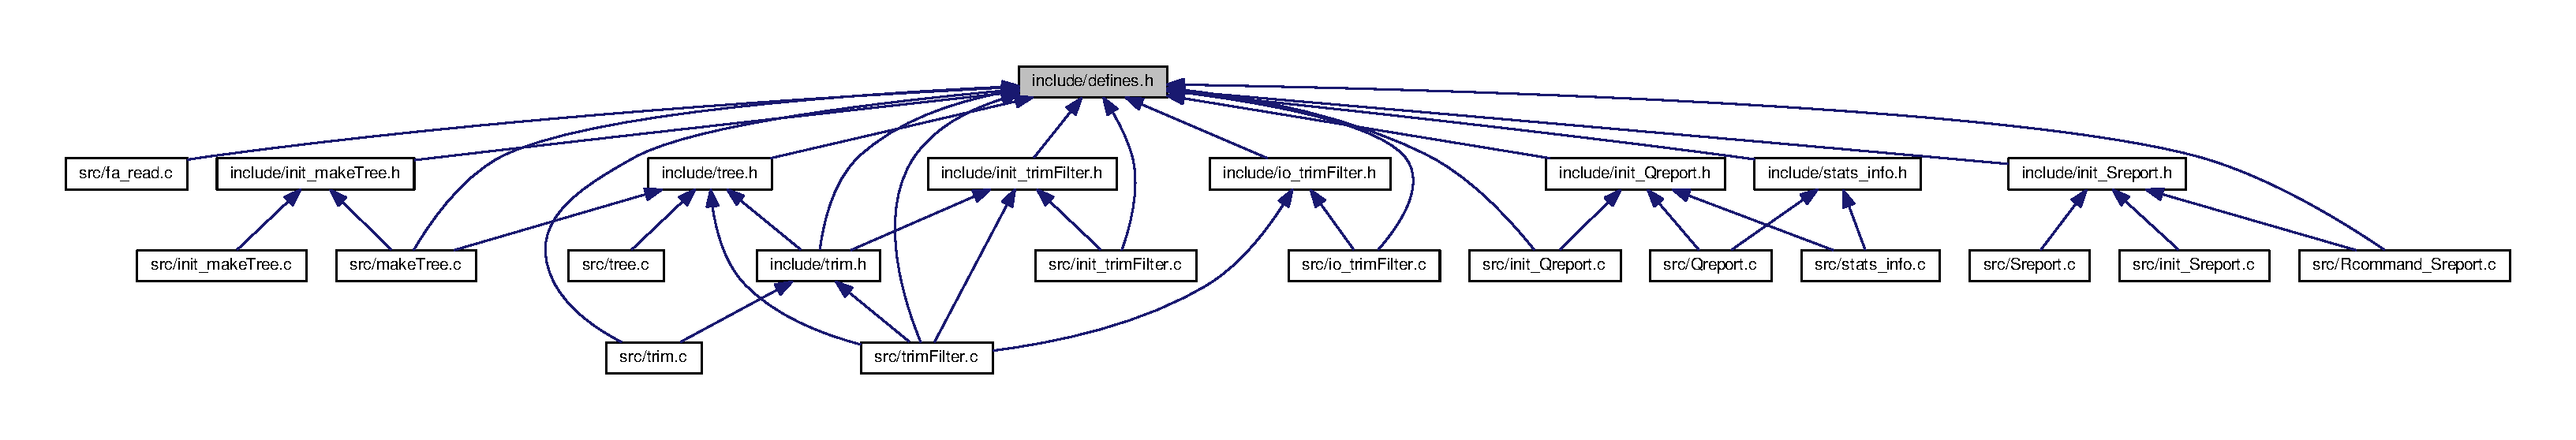
\includegraphics[width=350pt]{defines_8h__dep__incl}
\end{center}
\end{figure}
\subsection*{Macros}
\begin{DoxyCompactItemize}
\item 
\#define \hyperlink{defines_8h_a4419cb9bb22330d00cfd4727a05060dd}{B\+\_\+\+L\+E\+N}~131072
\item 
\#define \hyperlink{defines_8h_abe0ec333b60117063f9b9fd9f849cb08}{M\+A\+X\+\_\+\+F\+I\+L\+E\+N\+A\+M\+E}~300
\item 
\#define \hyperlink{defines_8h_abb452686968e48b67397da5f97445f5b}{bool}~short
\item 
\#define \hyperlink{defines_8h_a41f9c5fb8b08eb5dc3edce4dcb37fee7}{true}~1
\item 
\#define \hyperlink{defines_8h_a65e9886d74aaee76545e83dd09011727}{false}~0
\item 
\#define \hyperlink{defines_8h_affe776513b24d84b39af8ab0930fef7f}{max}(a, b)~( ((a) $>$ (b)) ? (a) \+: (b) )
\item 
\#define \hyperlink{defines_8h_ac6afabdc09a49a433ee19d8a9486056d}{min}(a, b)~( ((a) $<$ (b)) ? (a) \+: (b) )
\item 
\#define \hyperlink{defines_8h_afb615637083826bc311382f50b9a112d}{mem\+\_\+usage\+M\+B}()
\item 
\#define \hyperlink{defines_8h_a3589a26d6b84700042e948056edb43f6}{mem\+\_\+usage}()
\item 
\#define \hyperlink{defines_8h_a5c35b08af4e6a3b09783354fcd255b79}{D\+E\+F\+A\+U\+L\+T\+\_\+\+M\+I\+N\+Q}~27
\item 
\#define \hyperlink{defines_8h_ad27320ae41ed8a200b4379d022dd3d2e}{D\+E\+F\+A\+U\+L\+T\+\_\+\+N\+T\+I\+L\+E\+S}~96
\item 
\#define \hyperlink{defines_8h_afc545fae88ff3e374926c51cc44ff4e1}{D\+E\+F\+A\+U\+L\+T\+\_\+\+N\+Q}~46
\item 
\#define \hyperlink{defines_8h_aa98062065af56c6cd07cc43f35ef7aad}{Z\+E\+R\+O\+Q}~33
\item 
\#define \hyperlink{defines_8h_a71b6eab2a5d9fd457d48f50869a888f6}{N\+\_\+\+A\+C\+G\+T}~5
\item 
\#define \hyperlink{defines_8h_ac95fc8ee3f8ffd70f4564bcdc813ae2d}{M\+A\+X\+\_\+\+R\+C\+O\+M\+M\+A\+N\+D}~4000
\item 
\#define \hyperlink{defines_8h_a305c0ce0ef65658d5c81329adf54294f}{F\+A\+\_\+\+E\+N\+T\+R\+Y\+\_\+\+B\+U\+F}~20
\item 
\#define \hyperlink{defines_8h_a3919067d6defd46504313402bac82d22}{T\+\_\+\+A\+C\+G\+T}~4
\item 
\#define \hyperlink{defines_8h_a4d1f3741d002e1c5367ca1e87ee103ae}{N\+P\+O\+O\+L\+\_\+1\+D}~1048576
\item 
\#define \hyperlink{defines_8h_aaaa0c4d9e8b67e3f38fb68b27baca056}{N\+P\+O\+O\+L\+\_\+2\+D}~16
\item 
\#define \hyperlink{defines_8h_aba3b47d51c7ee08d2e0e92e58aa07106}{M\+A\+X\+\_\+\+F\+A\+S\+Z\+\_\+\+T\+R\+E\+E}~1e7
\item 
\#define \hyperlink{defines_8h_acd2baa2e68a76c64752672c201fff29a}{B\+I\+T\+S\+P\+E\+R\+C\+H\+A\+R}~8
\item 
\#define \hyperlink{defines_8h_a6722ebf83f6f843343b21592e3cd86ed}{B\+A\+S\+E\+S\+P\+E\+R\+C\+H\+A\+R}~4
\item 
\#define \hyperlink{defines_8h_a53c139d8ab18ed3e13ff65f63067fcac}{K\+M\+E\+R\+\_\+\+L\+E\+N}~25
\item 
\#define \hyperlink{defines_8h_ad9cbfc308e2064d4cc62c835753a39ea}{F\+A\+L\+S\+E\+\_\+\+P\+O\+S\+\_\+\+R\+A\+T\+E}~0.\+05
\item 
\#define \hyperlink{defines_8h_a78ea345c3971e9f004f71b15dda31d37}{Z\+E\+R\+O\+\_\+\+P\+O\+S\+\_\+\+R\+A\+T\+E}~1e-\/14
\item 
\#define \hyperlink{defines_8h_a996bde01ecac342918f0a2c4e7ce7bd5}{N\+O}~0
\item 
\#define \hyperlink{defines_8h_a1edd1ea8bddaf4d9c5eb3eae1ee1726a}{A\+L\+L}~1
\item 
\#define \hyperlink{defines_8h_a052e72209cfac2ff9aa78294f0bebea8}{E\+N\+D\+S}~2
\item 
\#define \hyperlink{defines_8h_a53529d9638a1d70f6e5989dedf4c2672}{S\+T\+R\+I\+P}~3
\item 
\#define \hyperlink{defines_8h_a653af6bd29f56a2699de26a928820da7}{F\+R\+A\+C}~3
\item 
\#define \hyperlink{defines_8h_abf0b71573c7ffc4f6746c24c9abc202a}{E\+N\+D\+S\+F\+R\+A\+C}~4
\item 
\#define \hyperlink{defines_8h_a3de33738fd3c7e77bffbcfaefc3e7645}{G\+L\+O\+B\+A\+L}~5
\item 
\#define \hyperlink{defines_8h_abf5b8fbbeb8255336e401a15a80214a8}{T\+R\+E\+E}~1
\item 
\#define \hyperlink{defines_8h_a1e43924adac4ae865aa0acf79710261c}{S\+A}~2
\item 
\#define \hyperlink{defines_8h_a7dcb6cfd9e186d997dce1d6cabe58898}{B\+L\+O\+O\+M}~3
\item 
\#define \hyperlink{defines_8h_a8fe83ac76edc595f6b98cd4a4127aed5}{E\+R\+R\+O\+R}~1000
\item 
\#define \hyperlink{defines_8h_a7fcff0e388619a194fb57f65c1053944}{D\+E\+F\+A\+U\+L\+T\+\_\+\+M\+I\+N\+L}~25
\item 
\#define \hyperlink{defines_8h_a50b2092be2f53229fda4d54644214af7}{A\+D\+A\+P}~0
\item 
\#define \hyperlink{defines_8h_a60519a721b44bce2b05a70cfa7ae8a1b}{C\+O\+N\+T}~1
\item 
\#define \hyperlink{defines_8h_a88236da90fdc203156cd02218f106f25}{L\+O\+W\+Q}~2
\item 
\#define \hyperlink{defines_8h_afdad8e3654b5f02ff4c50fcb88f6eed9}{N\+N\+N\+N}~3
\item 
\#define \hyperlink{defines_8h_a4adf7c6105c54a1608753548236d1387}{G\+O\+O\+D}~4
\item 
\#define \hyperlink{defines_8h_a23f1103d8247781ab0be4b0fba2f085f}{N\+F\+I\+L\+T\+E\+R\+S}~4
\end{DoxyCompactItemize}


\subsection{Detailed Description}
Macro definitions. 

\begin{DoxyAuthor}{Author}
Paula Perez \href{mailto:paulaperezrubio@gmail.com}{\tt paulaperezrubio@gmail.\+com} 
\end{DoxyAuthor}
\begin{DoxyDate}{Date}
07.\+08.\+2017 
\end{DoxyDate}


\subsection{Macro Definition Documentation}
\hypertarget{defines_8h_a50b2092be2f53229fda4d54644214af7}{\index{defines.\+h@{defines.\+h}!A\+D\+A\+P@{A\+D\+A\+P}}
\index{A\+D\+A\+P@{A\+D\+A\+P}!defines.\+h@{defines.\+h}}
\subsubsection[{A\+D\+A\+P}]{\setlength{\rightskip}{0pt plus 5cm}\#define A\+D\+A\+P~0}}\label{defines_8h_a50b2092be2f53229fda4d54644214af7}
Adapter filter \hypertarget{defines_8h_a1edd1ea8bddaf4d9c5eb3eae1ee1726a}{\index{defines.\+h@{defines.\+h}!A\+L\+L@{A\+L\+L}}
\index{A\+L\+L@{A\+L\+L}!defines.\+h@{defines.\+h}}
\subsubsection[{A\+L\+L}]{\setlength{\rightskip}{0pt plus 5cm}\#define A\+L\+L~1}}\label{defines_8h_a1edd1ea8bddaf4d9c5eb3eae1ee1726a}
Trims if a low\+Q base calling $\vert$ N is found \hypertarget{defines_8h_a4419cb9bb22330d00cfd4727a05060dd}{\index{defines.\+h@{defines.\+h}!B\+\_\+\+L\+E\+N@{B\+\_\+\+L\+E\+N}}
\index{B\+\_\+\+L\+E\+N@{B\+\_\+\+L\+E\+N}!defines.\+h@{defines.\+h}}
\subsubsection[{B\+\_\+\+L\+E\+N}]{\setlength{\rightskip}{0pt plus 5cm}\#define B\+\_\+\+L\+E\+N~131072}}\label{defines_8h_a4419cb9bb22330d00cfd4727a05060dd}
buffer size \hypertarget{defines_8h_a6722ebf83f6f843343b21592e3cd86ed}{\index{defines.\+h@{defines.\+h}!B\+A\+S\+E\+S\+P\+E\+R\+C\+H\+A\+R@{B\+A\+S\+E\+S\+P\+E\+R\+C\+H\+A\+R}}
\index{B\+A\+S\+E\+S\+P\+E\+R\+C\+H\+A\+R@{B\+A\+S\+E\+S\+P\+E\+R\+C\+H\+A\+R}!defines.\+h@{defines.\+h}}
\subsubsection[{B\+A\+S\+E\+S\+P\+E\+R\+C\+H\+A\+R}]{\setlength{\rightskip}{0pt plus 5cm}\#define B\+A\+S\+E\+S\+P\+E\+R\+C\+H\+A\+R~4}}\label{defines_8h_a6722ebf83f6f843343b21592e3cd86ed}
number of nucleotides that can fit in a char \hypertarget{defines_8h_acd2baa2e68a76c64752672c201fff29a}{\index{defines.\+h@{defines.\+h}!B\+I\+T\+S\+P\+E\+R\+C\+H\+A\+R@{B\+I\+T\+S\+P\+E\+R\+C\+H\+A\+R}}
\index{B\+I\+T\+S\+P\+E\+R\+C\+H\+A\+R@{B\+I\+T\+S\+P\+E\+R\+C\+H\+A\+R}!defines.\+h@{defines.\+h}}
\subsubsection[{B\+I\+T\+S\+P\+E\+R\+C\+H\+A\+R}]{\setlength{\rightskip}{0pt plus 5cm}\#define B\+I\+T\+S\+P\+E\+R\+C\+H\+A\+R~8}}\label{defines_8h_acd2baa2e68a76c64752672c201fff29a}
number of bits in a char \hypertarget{defines_8h_a7dcb6cfd9e186d997dce1d6cabe58898}{\index{defines.\+h@{defines.\+h}!B\+L\+O\+O\+M@{B\+L\+O\+O\+M}}
\index{B\+L\+O\+O\+M@{B\+L\+O\+O\+M}!defines.\+h@{defines.\+h}}
\subsubsection[{B\+L\+O\+O\+M}]{\setlength{\rightskip}{0pt plus 5cm}\#define B\+L\+O\+O\+M~3}}\label{defines_8h_a7dcb6cfd9e186d997dce1d6cabe58898}
Use a bloom filter to look for contaminations \hypertarget{defines_8h_abb452686968e48b67397da5f97445f5b}{\index{defines.\+h@{defines.\+h}!bool@{bool}}
\index{bool@{bool}!defines.\+h@{defines.\+h}}
\subsubsection[{bool}]{\setlength{\rightskip}{0pt plus 5cm}\#define bool~short}}\label{defines_8h_abb452686968e48b67397da5f97445f5b}
define a bool type \hypertarget{defines_8h_a60519a721b44bce2b05a70cfa7ae8a1b}{\index{defines.\+h@{defines.\+h}!C\+O\+N\+T@{C\+O\+N\+T}}
\index{C\+O\+N\+T@{C\+O\+N\+T}!defines.\+h@{defines.\+h}}
\subsubsection[{C\+O\+N\+T}]{\setlength{\rightskip}{0pt plus 5cm}\#define C\+O\+N\+T~1}}\label{defines_8h_a60519a721b44bce2b05a70cfa7ae8a1b}
Contamination filter \hypertarget{defines_8h_a7fcff0e388619a194fb57f65c1053944}{\index{defines.\+h@{defines.\+h}!D\+E\+F\+A\+U\+L\+T\+\_\+\+M\+I\+N\+L@{D\+E\+F\+A\+U\+L\+T\+\_\+\+M\+I\+N\+L}}
\index{D\+E\+F\+A\+U\+L\+T\+\_\+\+M\+I\+N\+L@{D\+E\+F\+A\+U\+L\+T\+\_\+\+M\+I\+N\+L}!defines.\+h@{defines.\+h}}
\subsubsection[{D\+E\+F\+A\+U\+L\+T\+\_\+\+M\+I\+N\+L}]{\setlength{\rightskip}{0pt plus 5cm}\#define D\+E\+F\+A\+U\+L\+T\+\_\+\+M\+I\+N\+L~25}}\label{defines_8h_a7fcff0e388619a194fb57f65c1053944}
Default minimum length under which we discard the reads \hypertarget{defines_8h_a5c35b08af4e6a3b09783354fcd255b79}{\index{defines.\+h@{defines.\+h}!D\+E\+F\+A\+U\+L\+T\+\_\+\+M\+I\+N\+Q@{D\+E\+F\+A\+U\+L\+T\+\_\+\+M\+I\+N\+Q}}
\index{D\+E\+F\+A\+U\+L\+T\+\_\+\+M\+I\+N\+Q@{D\+E\+F\+A\+U\+L\+T\+\_\+\+M\+I\+N\+Q}!defines.\+h@{defines.\+h}}
\subsubsection[{D\+E\+F\+A\+U\+L\+T\+\_\+\+M\+I\+N\+Q}]{\setlength{\rightskip}{0pt plus 5cm}\#define D\+E\+F\+A\+U\+L\+T\+\_\+\+M\+I\+N\+Q~27}}\label{defines_8h_a5c35b08af4e6a3b09783354fcd255b79}
Minimum quality threshold \hypertarget{defines_8h_afc545fae88ff3e374926c51cc44ff4e1}{\index{defines.\+h@{defines.\+h}!D\+E\+F\+A\+U\+L\+T\+\_\+\+N\+Q@{D\+E\+F\+A\+U\+L\+T\+\_\+\+N\+Q}}
\index{D\+E\+F\+A\+U\+L\+T\+\_\+\+N\+Q@{D\+E\+F\+A\+U\+L\+T\+\_\+\+N\+Q}!defines.\+h@{defines.\+h}}
\subsubsection[{D\+E\+F\+A\+U\+L\+T\+\_\+\+N\+Q}]{\setlength{\rightskip}{0pt plus 5cm}\#define D\+E\+F\+A\+U\+L\+T\+\_\+\+N\+Q~46}}\label{defines_8h_afc545fae88ff3e374926c51cc44ff4e1}
Default number of different quality values \hypertarget{defines_8h_ad27320ae41ed8a200b4379d022dd3d2e}{\index{defines.\+h@{defines.\+h}!D\+E\+F\+A\+U\+L\+T\+\_\+\+N\+T\+I\+L\+E\+S@{D\+E\+F\+A\+U\+L\+T\+\_\+\+N\+T\+I\+L\+E\+S}}
\index{D\+E\+F\+A\+U\+L\+T\+\_\+\+N\+T\+I\+L\+E\+S@{D\+E\+F\+A\+U\+L\+T\+\_\+\+N\+T\+I\+L\+E\+S}!defines.\+h@{defines.\+h}}
\subsubsection[{D\+E\+F\+A\+U\+L\+T\+\_\+\+N\+T\+I\+L\+E\+S}]{\setlength{\rightskip}{0pt plus 5cm}\#define D\+E\+F\+A\+U\+L\+T\+\_\+\+N\+T\+I\+L\+E\+S~96}}\label{defines_8h_ad27320ae41ed8a200b4379d022dd3d2e}
Default number of tiles \hypertarget{defines_8h_a052e72209cfac2ff9aa78294f0bebea8}{\index{defines.\+h@{defines.\+h}!E\+N\+D\+S@{E\+N\+D\+S}}
\index{E\+N\+D\+S@{E\+N\+D\+S}!defines.\+h@{defines.\+h}}
\subsubsection[{E\+N\+D\+S}]{\setlength{\rightskip}{0pt plus 5cm}\#define E\+N\+D\+S~2}}\label{defines_8h_a052e72209cfac2ff9aa78294f0bebea8}
Trims at the ends \hypertarget{defines_8h_abf0b71573c7ffc4f6746c24c9abc202a}{\index{defines.\+h@{defines.\+h}!E\+N\+D\+S\+F\+R\+A\+C@{E\+N\+D\+S\+F\+R\+A\+C}}
\index{E\+N\+D\+S\+F\+R\+A\+C@{E\+N\+D\+S\+F\+R\+A\+C}!defines.\+h@{defines.\+h}}
\subsubsection[{E\+N\+D\+S\+F\+R\+A\+C}]{\setlength{\rightskip}{0pt plus 5cm}\#define E\+N\+D\+S\+F\+R\+A\+C~4}}\label{defines_8h_abf0b71573c7ffc4f6746c24c9abc202a}
trims at the ends and discards a read if the remaining part has more than $>$ percent low\+Q bases \hypertarget{defines_8h_a8fe83ac76edc595f6b98cd4a4127aed5}{\index{defines.\+h@{defines.\+h}!E\+R\+R\+O\+R@{E\+R\+R\+O\+R}}
\index{E\+R\+R\+O\+R@{E\+R\+R\+O\+R}!defines.\+h@{defines.\+h}}
\subsubsection[{E\+R\+R\+O\+R}]{\setlength{\rightskip}{0pt plus 5cm}\#define E\+R\+R\+O\+R~1000}}\label{defines_8h_a8fe83ac76edc595f6b98cd4a4127aed5}
Encodes an error when reading in trim\+N, trim\+Q, method options in trim\+Filter \hypertarget{defines_8h_a305c0ce0ef65658d5c81329adf54294f}{\index{defines.\+h@{defines.\+h}!F\+A\+\_\+\+E\+N\+T\+R\+Y\+\_\+\+B\+U\+F@{F\+A\+\_\+\+E\+N\+T\+R\+Y\+\_\+\+B\+U\+F}}
\index{F\+A\+\_\+\+E\+N\+T\+R\+Y\+\_\+\+B\+U\+F@{F\+A\+\_\+\+E\+N\+T\+R\+Y\+\_\+\+B\+U\+F}!defines.\+h@{defines.\+h}}
\subsubsection[{F\+A\+\_\+\+E\+N\+T\+R\+Y\+\_\+\+B\+U\+F}]{\setlength{\rightskip}{0pt plus 5cm}\#define F\+A\+\_\+\+E\+N\+T\+R\+Y\+\_\+\+B\+U\+F~20}}\label{defines_8h_a305c0ce0ef65658d5c81329adf54294f}
buffer for fasta entries \hypertarget{defines_8h_a65e9886d74aaee76545e83dd09011727}{\index{defines.\+h@{defines.\+h}!false@{false}}
\index{false@{false}!defines.\+h@{defines.\+h}}
\subsubsection[{false}]{\setlength{\rightskip}{0pt plus 5cm}\#define false~0}}\label{defines_8h_a65e9886d74aaee76545e83dd09011727}
assign false to 0 \hypertarget{defines_8h_ad9cbfc308e2064d4cc62c835753a39ea}{\index{defines.\+h@{defines.\+h}!F\+A\+L\+S\+E\+\_\+\+P\+O\+S\+\_\+\+R\+A\+T\+E@{F\+A\+L\+S\+E\+\_\+\+P\+O\+S\+\_\+\+R\+A\+T\+E}}
\index{F\+A\+L\+S\+E\+\_\+\+P\+O\+S\+\_\+\+R\+A\+T\+E@{F\+A\+L\+S\+E\+\_\+\+P\+O\+S\+\_\+\+R\+A\+T\+E}!defines.\+h@{defines.\+h}}
\subsubsection[{F\+A\+L\+S\+E\+\_\+\+P\+O\+S\+\_\+\+R\+A\+T\+E}]{\setlength{\rightskip}{0pt plus 5cm}\#define F\+A\+L\+S\+E\+\_\+\+P\+O\+S\+\_\+\+R\+A\+T\+E~0.\+05}}\label{defines_8h_ad9cbfc308e2064d4cc62c835753a39ea}
default false positive rate \hypertarget{defines_8h_a653af6bd29f56a2699de26a928820da7}{\index{defines.\+h@{defines.\+h}!F\+R\+A\+C@{F\+R\+A\+C}}
\index{F\+R\+A\+C@{F\+R\+A\+C}!defines.\+h@{defines.\+h}}
\subsubsection[{F\+R\+A\+C}]{\setlength{\rightskip}{0pt plus 5cm}\#define F\+R\+A\+C~3}}\label{defines_8h_a653af6bd29f56a2699de26a928820da7}
Discards a read if it contains $>$ percent low\+Q bases \hypertarget{defines_8h_a3de33738fd3c7e77bffbcfaefc3e7645}{\index{defines.\+h@{defines.\+h}!G\+L\+O\+B\+A\+L@{G\+L\+O\+B\+A\+L}}
\index{G\+L\+O\+B\+A\+L@{G\+L\+O\+B\+A\+L}!defines.\+h@{defines.\+h}}
\subsubsection[{G\+L\+O\+B\+A\+L}]{\setlength{\rightskip}{0pt plus 5cm}\#define G\+L\+O\+B\+A\+L~5}}\label{defines_8h_a3de33738fd3c7e77bffbcfaefc3e7645}
Trims a fixed \# bases from e left and right \hypertarget{defines_8h_a4adf7c6105c54a1608753548236d1387}{\index{defines.\+h@{defines.\+h}!G\+O\+O\+D@{G\+O\+O\+D}}
\index{G\+O\+O\+D@{G\+O\+O\+D}!defines.\+h@{defines.\+h}}
\subsubsection[{G\+O\+O\+D}]{\setlength{\rightskip}{0pt plus 5cm}\#define G\+O\+O\+D~4}}\label{defines_8h_a4adf7c6105c54a1608753548236d1387}
Good reads \hypertarget{defines_8h_a53c139d8ab18ed3e13ff65f63067fcac}{\index{defines.\+h@{defines.\+h}!K\+M\+E\+R\+\_\+\+L\+E\+N@{K\+M\+E\+R\+\_\+\+L\+E\+N}}
\index{K\+M\+E\+R\+\_\+\+L\+E\+N@{K\+M\+E\+R\+\_\+\+L\+E\+N}!defines.\+h@{defines.\+h}}
\subsubsection[{K\+M\+E\+R\+\_\+\+L\+E\+N}]{\setlength{\rightskip}{0pt plus 5cm}\#define K\+M\+E\+R\+\_\+\+L\+E\+N~25}}\label{defines_8h_a53c139d8ab18ed3e13ff65f63067fcac}
default kmer length \hypertarget{defines_8h_a88236da90fdc203156cd02218f106f25}{\index{defines.\+h@{defines.\+h}!L\+O\+W\+Q@{L\+O\+W\+Q}}
\index{L\+O\+W\+Q@{L\+O\+W\+Q}!defines.\+h@{defines.\+h}}
\subsubsection[{L\+O\+W\+Q}]{\setlength{\rightskip}{0pt plus 5cm}\#define L\+O\+W\+Q~2}}\label{defines_8h_a88236da90fdc203156cd02218f106f25}
Low quality filter \hypertarget{defines_8h_affe776513b24d84b39af8ab0930fef7f}{\index{defines.\+h@{defines.\+h}!max@{max}}
\index{max@{max}!defines.\+h@{defines.\+h}}
\subsubsection[{max}]{\setlength{\rightskip}{0pt plus 5cm}\#define max(
\begin{DoxyParamCaption}
\item[{}]{a, }
\item[{}]{b}
\end{DoxyParamCaption}
)~( ((a) $>$ (b)) ? (a) \+: (b) )}}\label{defines_8h_affe776513b24d84b39af8ab0930fef7f}
max function \hypertarget{defines_8h_aba3b47d51c7ee08d2e0e92e58aa07106}{\index{defines.\+h@{defines.\+h}!M\+A\+X\+\_\+\+F\+A\+S\+Z\+\_\+\+T\+R\+E\+E@{M\+A\+X\+\_\+\+F\+A\+S\+Z\+\_\+\+T\+R\+E\+E}}
\index{M\+A\+X\+\_\+\+F\+A\+S\+Z\+\_\+\+T\+R\+E\+E@{M\+A\+X\+\_\+\+F\+A\+S\+Z\+\_\+\+T\+R\+E\+E}!defines.\+h@{defines.\+h}}
\subsubsection[{M\+A\+X\+\_\+\+F\+A\+S\+Z\+\_\+\+T\+R\+E\+E}]{\setlength{\rightskip}{0pt plus 5cm}\#define M\+A\+X\+\_\+\+F\+A\+S\+Z\+\_\+\+T\+R\+E\+E~1e7}}\label{defines_8h_aba3b47d51c7ee08d2e0e92e58aa07106}
Maximum fasta size for constructing a tree. D\+E\+C\+I\+D\+E A S\+E\+N\+S\+I\+B\+L\+E S\+I\+Z\+E! \hypertarget{defines_8h_abe0ec333b60117063f9b9fd9f849cb08}{\index{defines.\+h@{defines.\+h}!M\+A\+X\+\_\+\+F\+I\+L\+E\+N\+A\+M\+E@{M\+A\+X\+\_\+\+F\+I\+L\+E\+N\+A\+M\+E}}
\index{M\+A\+X\+\_\+\+F\+I\+L\+E\+N\+A\+M\+E@{M\+A\+X\+\_\+\+F\+I\+L\+E\+N\+A\+M\+E}!defines.\+h@{defines.\+h}}
\subsubsection[{M\+A\+X\+\_\+\+F\+I\+L\+E\+N\+A\+M\+E}]{\setlength{\rightskip}{0pt plus 5cm}\#define M\+A\+X\+\_\+\+F\+I\+L\+E\+N\+A\+M\+E~300}}\label{defines_8h_abe0ec333b60117063f9b9fd9f849cb08}
Maximum \# chars in a filename \hypertarget{defines_8h_ac95fc8ee3f8ffd70f4564bcdc813ae2d}{\index{defines.\+h@{defines.\+h}!M\+A\+X\+\_\+\+R\+C\+O\+M\+M\+A\+N\+D@{M\+A\+X\+\_\+\+R\+C\+O\+M\+M\+A\+N\+D}}
\index{M\+A\+X\+\_\+\+R\+C\+O\+M\+M\+A\+N\+D@{M\+A\+X\+\_\+\+R\+C\+O\+M\+M\+A\+N\+D}!defines.\+h@{defines.\+h}}
\subsubsection[{M\+A\+X\+\_\+\+R\+C\+O\+M\+M\+A\+N\+D}]{\setlength{\rightskip}{0pt plus 5cm}\#define M\+A\+X\+\_\+\+R\+C\+O\+M\+M\+A\+N\+D~4000}}\label{defines_8h_ac95fc8ee3f8ffd70f4564bcdc813ae2d}
Maximum \# chars in R command \hypertarget{defines_8h_a3589a26d6b84700042e948056edb43f6}{\index{defines.\+h@{defines.\+h}!mem\+\_\+usage@{mem\+\_\+usage}}
\index{mem\+\_\+usage@{mem\+\_\+usage}!defines.\+h@{defines.\+h}}
\subsubsection[{mem\+\_\+usage}]{\setlength{\rightskip}{0pt plus 5cm}\#define mem\+\_\+usage(
\begin{DoxyParamCaption}
{}
\end{DoxyParamCaption}
)}}\label{defines_8h_a3589a26d6b84700042e948056edb43f6}
{\bfseries Value\+:}
\begin{DoxyCode}
fprintf(stderr, \(\backslash\)
         \textcolor{stringliteral}{"- Current allocated memory: %ld Bytes.\(\backslash\)n"}, \(\backslash\)
         \hyperlink{bloom_8c_aaa0ac3ef63b80a6bf32b2cffd17ceb0f}{alloc\_mem})
\end{DoxyCode}
returns allocated memory in Bytes \hypertarget{defines_8h_afb615637083826bc311382f50b9a112d}{\index{defines.\+h@{defines.\+h}!mem\+\_\+usage\+M\+B@{mem\+\_\+usage\+M\+B}}
\index{mem\+\_\+usage\+M\+B@{mem\+\_\+usage\+M\+B}!defines.\+h@{defines.\+h}}
\subsubsection[{mem\+\_\+usage\+M\+B}]{\setlength{\rightskip}{0pt plus 5cm}\#define mem\+\_\+usage\+M\+B(
\begin{DoxyParamCaption}
{}
\end{DoxyParamCaption}
)}}\label{defines_8h_afb615637083826bc311382f50b9a112d}
{\bfseries Value\+:}
\begin{DoxyCode}
fprintf(stderr, \(\backslash\)
         \textcolor{stringliteral}{"- Current allocated memory: %ld MB.\(\backslash\)n"}, \(\backslash\)
         \hyperlink{bloom_8c_aaa0ac3ef63b80a6bf32b2cffd17ceb0f}{alloc\_mem} >> 20)
\end{DoxyCode}
returns allocated memory in M\+B \hypertarget{defines_8h_ac6afabdc09a49a433ee19d8a9486056d}{\index{defines.\+h@{defines.\+h}!min@{min}}
\index{min@{min}!defines.\+h@{defines.\+h}}
\subsubsection[{min}]{\setlength{\rightskip}{0pt plus 5cm}\#define min(
\begin{DoxyParamCaption}
\item[{}]{a, }
\item[{}]{b}
\end{DoxyParamCaption}
)~( ((a) $<$ (b)) ? (a) \+: (b) )}}\label{defines_8h_ac6afabdc09a49a433ee19d8a9486056d}
min function \hypertarget{defines_8h_a71b6eab2a5d9fd457d48f50869a888f6}{\index{defines.\+h@{defines.\+h}!N\+\_\+\+A\+C\+G\+T@{N\+\_\+\+A\+C\+G\+T}}
\index{N\+\_\+\+A\+C\+G\+T@{N\+\_\+\+A\+C\+G\+T}!defines.\+h@{defines.\+h}}
\subsubsection[{N\+\_\+\+A\+C\+G\+T}]{\setlength{\rightskip}{0pt plus 5cm}\#define N\+\_\+\+A\+C\+G\+T~5}}\label{defines_8h_a71b6eab2a5d9fd457d48f50869a888f6}
Number of different nucleotides in the fq file \hypertarget{defines_8h_a23f1103d8247781ab0be4b0fba2f085f}{\index{defines.\+h@{defines.\+h}!N\+F\+I\+L\+T\+E\+R\+S@{N\+F\+I\+L\+T\+E\+R\+S}}
\index{N\+F\+I\+L\+T\+E\+R\+S@{N\+F\+I\+L\+T\+E\+R\+S}!defines.\+h@{defines.\+h}}
\subsubsection[{N\+F\+I\+L\+T\+E\+R\+S}]{\setlength{\rightskip}{0pt plus 5cm}\#define N\+F\+I\+L\+T\+E\+R\+S~4}}\label{defines_8h_a23f1103d8247781ab0be4b0fba2f085f}
total number of filters \hypertarget{defines_8h_afdad8e3654b5f02ff4c50fcb88f6eed9}{\index{defines.\+h@{defines.\+h}!N\+N\+N\+N@{N\+N\+N\+N}}
\index{N\+N\+N\+N@{N\+N\+N\+N}!defines.\+h@{defines.\+h}}
\subsubsection[{N\+N\+N\+N}]{\setlength{\rightskip}{0pt plus 5cm}\#define N\+N\+N\+N~3}}\label{defines_8h_afdad8e3654b5f02ff4c50fcb88f6eed9}
N's presence filter \hypertarget{defines_8h_a996bde01ecac342918f0a2c4e7ce7bd5}{\index{defines.\+h@{defines.\+h}!N\+O@{N\+O}}
\index{N\+O@{N\+O}!defines.\+h@{defines.\+h}}
\subsubsection[{N\+O}]{\setlength{\rightskip}{0pt plus 5cm}\#define N\+O~0}}\label{defines_8h_a996bde01ecac342918f0a2c4e7ce7bd5}
No trimming \hypertarget{defines_8h_a4d1f3741d002e1c5367ca1e87ee103ae}{\index{defines.\+h@{defines.\+h}!N\+P\+O\+O\+L\+\_\+1\+D@{N\+P\+O\+O\+L\+\_\+1\+D}}
\index{N\+P\+O\+O\+L\+\_\+1\+D@{N\+P\+O\+O\+L\+\_\+1\+D}!defines.\+h@{defines.\+h}}
\subsubsection[{N\+P\+O\+O\+L\+\_\+1\+D}]{\setlength{\rightskip}{0pt plus 5cm}\#define N\+P\+O\+O\+L\+\_\+1\+D~1048576}}\label{defines_8h_a4d1f3741d002e1c5367ca1e87ee103ae}
Number of Node structs allocated in inner dim \hypertarget{defines_8h_aaaa0c4d9e8b67e3f38fb68b27baca056}{\index{defines.\+h@{defines.\+h}!N\+P\+O\+O\+L\+\_\+2\+D@{N\+P\+O\+O\+L\+\_\+2\+D}}
\index{N\+P\+O\+O\+L\+\_\+2\+D@{N\+P\+O\+O\+L\+\_\+2\+D}!defines.\+h@{defines.\+h}}
\subsubsection[{N\+P\+O\+O\+L\+\_\+2\+D}]{\setlength{\rightskip}{0pt plus 5cm}\#define N\+P\+O\+O\+L\+\_\+2\+D~16}}\label{defines_8h_aaaa0c4d9e8b67e3f38fb68b27baca056}
Number of $\ast$\+Node allocated in outer dim \hypertarget{defines_8h_a1e43924adac4ae865aa0acf79710261c}{\index{defines.\+h@{defines.\+h}!S\+A@{S\+A}}
\index{S\+A@{S\+A}!defines.\+h@{defines.\+h}}
\subsubsection[{S\+A}]{\setlength{\rightskip}{0pt plus 5cm}\#define S\+A~2}}\label{defines_8h_a1e43924adac4ae865aa0acf79710261c}
Use a suffix array to look for contaminations \hypertarget{defines_8h_a53529d9638a1d70f6e5989dedf4c2672}{\index{defines.\+h@{defines.\+h}!S\+T\+R\+I\+P@{S\+T\+R\+I\+P}}
\index{S\+T\+R\+I\+P@{S\+T\+R\+I\+P}!defines.\+h@{defines.\+h}}
\subsubsection[{S\+T\+R\+I\+P}]{\setlength{\rightskip}{0pt plus 5cm}\#define S\+T\+R\+I\+P~3}}\label{defines_8h_a53529d9638a1d70f6e5989dedf4c2672}
Looks for the largest N-\/free sequence \hypertarget{defines_8h_a3919067d6defd46504313402bac82d22}{\index{defines.\+h@{defines.\+h}!T\+\_\+\+A\+C\+G\+T@{T\+\_\+\+A\+C\+G\+T}}
\index{T\+\_\+\+A\+C\+G\+T@{T\+\_\+\+A\+C\+G\+T}!defines.\+h@{defines.\+h}}
\subsubsection[{T\+\_\+\+A\+C\+G\+T}]{\setlength{\rightskip}{0pt plus 5cm}\#define T\+\_\+\+A\+C\+G\+T~4}}\label{defines_8h_a3919067d6defd46504313402bac82d22}
Number of children per node in tree \hypertarget{defines_8h_abf5b8fbbeb8255336e401a15a80214a8}{\index{defines.\+h@{defines.\+h}!T\+R\+E\+E@{T\+R\+E\+E}}
\index{T\+R\+E\+E@{T\+R\+E\+E}!defines.\+h@{defines.\+h}}
\subsubsection[{T\+R\+E\+E}]{\setlength{\rightskip}{0pt plus 5cm}\#define T\+R\+E\+E~1}}\label{defines_8h_abf5b8fbbeb8255336e401a15a80214a8}
Use a tree to look for contaminations \hypertarget{defines_8h_a41f9c5fb8b08eb5dc3edce4dcb37fee7}{\index{defines.\+h@{defines.\+h}!true@{true}}
\index{true@{true}!defines.\+h@{defines.\+h}}
\subsubsection[{true}]{\setlength{\rightskip}{0pt plus 5cm}\#define true~1}}\label{defines_8h_a41f9c5fb8b08eb5dc3edce4dcb37fee7}
assign true to 1 \hypertarget{defines_8h_a78ea345c3971e9f004f71b15dda31d37}{\index{defines.\+h@{defines.\+h}!Z\+E\+R\+O\+\_\+\+P\+O\+S\+\_\+\+R\+A\+T\+E@{Z\+E\+R\+O\+\_\+\+P\+O\+S\+\_\+\+R\+A\+T\+E}}
\index{Z\+E\+R\+O\+\_\+\+P\+O\+S\+\_\+\+R\+A\+T\+E@{Z\+E\+R\+O\+\_\+\+P\+O\+S\+\_\+\+R\+A\+T\+E}!defines.\+h@{defines.\+h}}
\subsubsection[{Z\+E\+R\+O\+\_\+\+P\+O\+S\+\_\+\+R\+A\+T\+E}]{\setlength{\rightskip}{0pt plus 5cm}\#define Z\+E\+R\+O\+\_\+\+P\+O\+S\+\_\+\+R\+A\+T\+E~1e-\/14}}\label{defines_8h_a78ea345c3971e9f004f71b15dda31d37}
0 threshold for a double \hypertarget{defines_8h_aa98062065af56c6cd07cc43f35ef7aad}{\index{defines.\+h@{defines.\+h}!Z\+E\+R\+O\+Q@{Z\+E\+R\+O\+Q}}
\index{Z\+E\+R\+O\+Q@{Z\+E\+R\+O\+Q}!defines.\+h@{defines.\+h}}
\subsubsection[{Z\+E\+R\+O\+Q}]{\setlength{\rightskip}{0pt plus 5cm}\#define Z\+E\+R\+O\+Q~33}}\label{defines_8h_aa98062065af56c6cd07cc43f35ef7aad}
A\+S\+C\+I\+I code of lowest quality value (!) 
\hypertarget{fopen__gen_8h}{\section{include/fopen\+\_\+gen.h File Reference}
\label{fopen__gen_8h}\index{include/fopen\+\_\+gen.\+h@{include/fopen\+\_\+gen.\+h}}
}


Uncompress/compress input/output files using pipes.  


{\ttfamily \#include $<$stdio.\+h$>$}\\*
Include dependency graph for fopen\+\_\+gen.\+h\+:\nopagebreak
\begin{figure}[H]
\begin{center}
\leavevmode
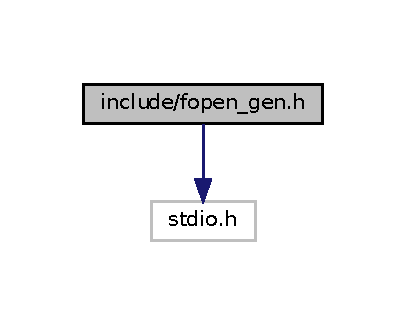
\includegraphics[width=184pt]{fopen__gen_8h__incl}
\end{center}
\end{figure}
This graph shows which files directly or indirectly include this file\+:\nopagebreak
\begin{figure}[H]
\begin{center}
\leavevmode
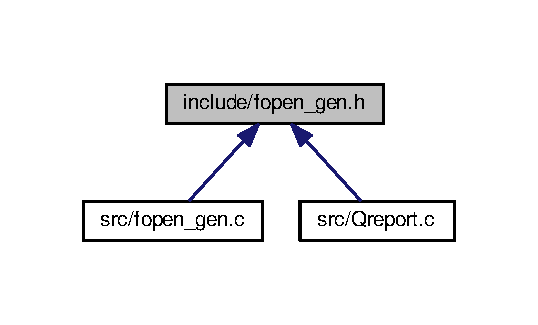
\includegraphics[width=258pt]{fopen__gen_8h__dep__incl}
\end{center}
\end{figure}
\subsection*{Macros}
\begin{DoxyCompactItemize}
\item 
\hypertarget{fopen__gen_8h_a2469c53816dc077f9deefb187ffcabf3}{\#define {\bfseries R\+E\+A\+D\+\_\+\+E\+N\+D}~0}\label{fopen__gen_8h_a2469c53816dc077f9deefb187ffcabf3}

\item 
\hypertarget{fopen__gen_8h_a2efd706d915e621e5e18b3f0803c4ed2}{\#define {\bfseries W\+R\+I\+T\+E\+\_\+\+E\+N\+D}~1}\label{fopen__gen_8h_a2efd706d915e621e5e18b3f0803c4ed2}

\item 
\hypertarget{fopen__gen_8h_a8b390f7305d3e2e82316936cde24101c}{\#define {\bfseries P\+E\+R\+M\+I\+S\+S\+I\+O\+N\+S}~0640}\label{fopen__gen_8h_a8b390f7305d3e2e82316936cde24101c}

\end{DoxyCompactItemize}
\subsection*{Functions}
\begin{DoxyCompactItemize}
\item 
\hypertarget{fopen__gen_8h_ae59755703d84f781f127762acf2deb6d}{int {\bfseries set\+Cloexec} (int fd)}\label{fopen__gen_8h_ae59755703d84f781f127762acf2deb6d}

\item 
F\+I\+L\+E $\ast$ \hyperlink{fopen__gen_8h_ae03fc1b9180f740dcb577fdb00072fb3}{fopen\+\_\+gen} (const char $\ast$path, const char $\ast$mode)
\begin{DoxyCompactList}\small\item\em Generalized fopen function. fopen\+\_\+gen is to be used as fopen. Can be used in read and in write mode. When used in read mode with a compressed extension, the file will be first decompressed and then read. When used in write mode with a compressed extension, the output will be compressed. \end{DoxyCompactList}\end{DoxyCompactItemize}


\subsection{Detailed Description}
Uncompress/compress input/output files using pipes. 

Hook the standard file opening functions, open, fopen and fopen64. If the extension of the file being opened indicates the file is compressed (.gz, .bz2, .xz), when opening in the reading mode a pipe to a program is opened that decompresses that file (gunzip, bunzip2 or xzdec) and return a handle to the open pipe. When opening in the writing mode (only for .gz, .bam), a pipe to a program is opened that compresses the output.

\begin{DoxyAuthor}{Author}
Paula Perez \href{mailto:paulaperezrubio@gmail.com}{\tt paulaperezrubio@gmail.\+com} 
\end{DoxyAuthor}
\begin{DoxyDate}{Date}
03.\+08.\+2017 
\end{DoxyDate}
\begin{DoxyWarning}{Warning}
vfork vs fork to be checked! 
\end{DoxyWarning}
\begin{DoxyNote}{Note}
-\/ original copyright note -\/ (reading mode, original C++ code) author\+: Shaun Jackman \href{mailto:sjackman@bcgsc.ca}{\tt sjackman@bcgsc.\+ca}, \href{https://github.com/bcgsc,}{\tt https\+://github.\+com/bcgsc,} filename\+: Uncompress.\+cpp 
\end{DoxyNote}


\subsection{Function Documentation}
\hypertarget{fopen__gen_8h_ae03fc1b9180f740dcb577fdb00072fb3}{\index{fopen\+\_\+gen.\+h@{fopen\+\_\+gen.\+h}!fopen\+\_\+gen@{fopen\+\_\+gen}}
\index{fopen\+\_\+gen@{fopen\+\_\+gen}!fopen\+\_\+gen.\+h@{fopen\+\_\+gen.\+h}}
\subsubsection[{fopen\+\_\+gen}]{\setlength{\rightskip}{0pt plus 5cm}F\+I\+L\+E$\ast$ fopen\+\_\+gen (
\begin{DoxyParamCaption}
\item[{const char $\ast$}]{path, }
\item[{const char $\ast$}]{mode}
\end{DoxyParamCaption}
)}}\label{fopen__gen_8h_ae03fc1b9180f740dcb577fdb00072fb3}


Generalized fopen function. fopen\+\_\+gen is to be used as fopen. Can be used in read and in write mode. When used in read mode with a compressed extension, the file will be first decompressed and then read. When used in write mode with a compressed extension, the output will be compressed. 

\begin{DoxyReturn}{Returns}
a F\+I\+L\+E pointer 
\end{DoxyReturn}

\hypertarget{fq__read_8h}{}\section{include/fq\+\_\+read.h File Reference}
\label{fq__read_8h}\index{include/fq\+\_\+read.\+h@{include/fq\+\_\+read.\+h}}


fastq entries manipulations (read/write)  


{\ttfamily \#include \char`\"{}config.\+h\char`\"{}}\newline
Include dependency graph for fq\+\_\+read.\+h\+:
\nopagebreak
\begin{figure}[H]
\begin{center}
\leavevmode
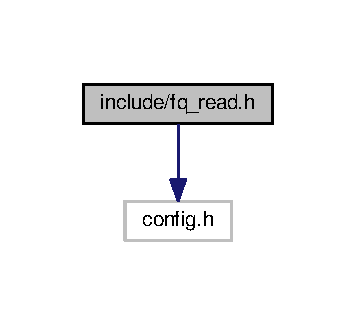
\includegraphics[width=181pt]{fq__read_8h__incl}
\end{center}
\end{figure}
This graph shows which files directly or indirectly include this file\+:
\nopagebreak
\begin{figure}[H]
\begin{center}
\leavevmode
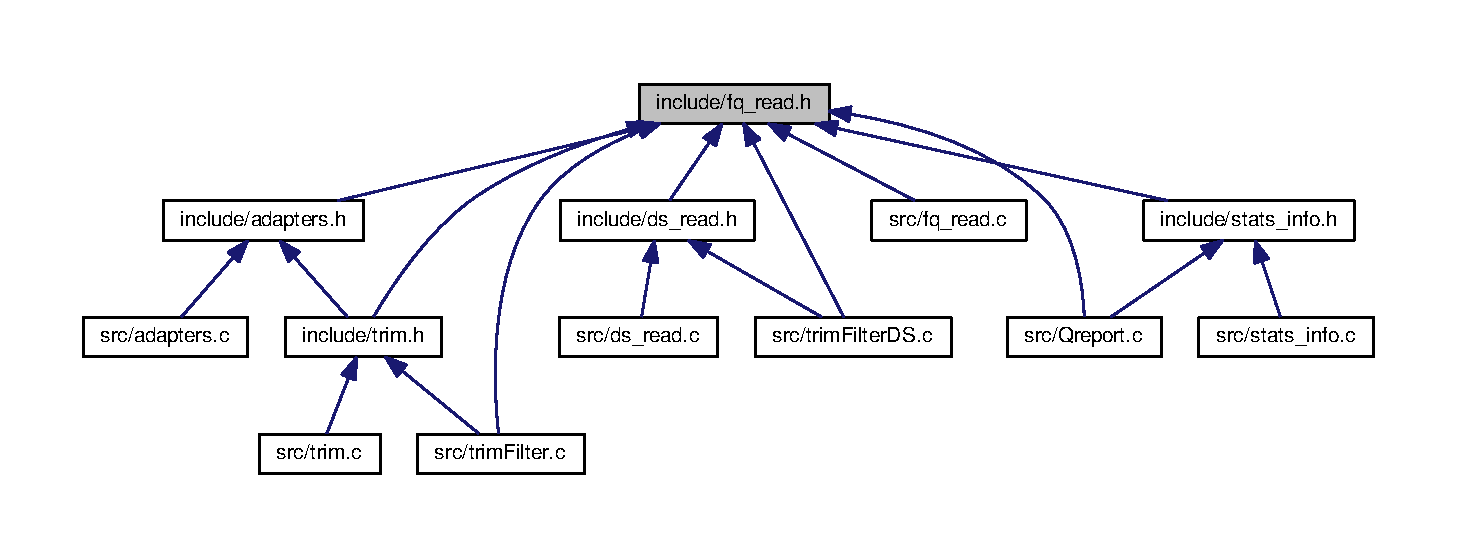
\includegraphics[width=350pt]{fq__read_8h__dep__incl}
\end{center}
\end{figure}
\subsection*{Classes}
\begin{DoxyCompactItemize}
\item 
struct \mbox{\hyperlink{struct__fq__read}{\+\_\+fq\+\_\+read}}
\begin{DoxyCompactList}\small\item\em stores a fastq entry \end{DoxyCompactList}\end{DoxyCompactItemize}
\subsection*{Typedefs}
\begin{DoxyCompactItemize}
\item 
\mbox{\Hypertarget{fq__read_8h_a9af37aa81397c9531c66863d4e97f034}\label{fq__read_8h_a9af37aa81397c9531c66863d4e97f034}} 
typedef struct \mbox{\hyperlink{struct__fq__read}{\+\_\+fq\+\_\+read}} \mbox{\hyperlink{fq__read_8h_a9af37aa81397c9531c66863d4e97f034}{Fq\+\_\+read}}
\begin{DoxyCompactList}\small\item\em stores a fastq entry \end{DoxyCompactList}\end{DoxyCompactItemize}
\subsection*{Functions}
\begin{DoxyCompactItemize}
\item 
int \mbox{\hyperlink{fq__read_8h_af0d30098d51bea3d11c442c3dd60e15f}{get\+\_\+fqread}} (\mbox{\hyperlink{fq__read_8h_a9af37aa81397c9531c66863d4e97f034}{Fq\+\_\+read}} $\ast$seq, char $\ast$buffer, int pos1, int pos2, int nline, int read\+\_\+len, int filter)
\begin{DoxyCompactList}\small\item\em reads fastq line from a buffer \end{DoxyCompactList}\item 
int \mbox{\hyperlink{fq__read_8h_ae58e185777143cd1fc4c75fccd5c647a}{string\+\_\+seq}} (\mbox{\hyperlink{fq__read_8h_a9af37aa81397c9531c66863d4e97f034}{Fq\+\_\+read}} $\ast$seq, char $\ast$char\+\_\+seq)
\begin{DoxyCompactList}\small\item\em writes the fq entry in a string \end{DoxyCompactList}\end{DoxyCompactItemize}


\subsection{Detailed Description}
fastq entries manipulations (read/write) 

\begin{DoxyAuthor}{Author}
Paula Perez \href{mailto:paulaperezrubio@gmail.com}{\tt paulaperezrubio@gmail.\+com} 
\end{DoxyAuthor}
\begin{DoxyDate}{Date}
03.\+08.\+2017 
\end{DoxyDate}


\subsection{Function Documentation}
\mbox{\Hypertarget{fq__read_8h_af0d30098d51bea3d11c442c3dd60e15f}\label{fq__read_8h_af0d30098d51bea3d11c442c3dd60e15f}} 
\index{fq\+\_\+read.\+h@{fq\+\_\+read.\+h}!get\+\_\+fqread@{get\+\_\+fqread}}
\index{get\+\_\+fqread@{get\+\_\+fqread}!fq\+\_\+read.\+h@{fq\+\_\+read.\+h}}
\subsubsection{\texorpdfstring{get\+\_\+fqread()}{get\_fqread()}}
{\footnotesize\ttfamily int get\+\_\+fqread (\begin{DoxyParamCaption}\item[{\mbox{\hyperlink{fq__read_8h_a9af37aa81397c9531c66863d4e97f034}{Fq\+\_\+read}} $\ast$}]{seq,  }\item[{char $\ast$}]{buffer,  }\item[{int}]{pos1,  }\item[{int}]{pos2,  }\item[{int}]{nline,  }\item[{int}]{read\+\_\+len,  }\item[{int}]{filter }\end{DoxyParamCaption})}



reads fastq line from a buffer 

a fastq line is read from a buffer and the relevant information is stored in a structure {\bfseries Fq\+\_\+read}. Depending on the value of {\bfseries filter}, information about whether the read was trimmed is stored.


\begin{DoxyParams}{Parameters}
{\em seq} & pointer to {\bfseries Fq\+\_\+read}, where the info will be stored. \\
\hline
{\em buffer} & variable where the file being read is stored. \\
\hline
{\em pos1} & buffer start position of the line. \\
\hline
{\em pos2} & buffer end position of the line. \\
\hline
{\em nline} & file line number being read. \\
\hline
{\em read\+\_\+len} & predefined read length \\
\hline
{\em filter} & 0 original file, 1 file filtered with filter\+\_\+trim, 2 file filtered with another tool \\
\hline
\end{DoxyParams}
\mbox{\Hypertarget{fq__read_8h_ae58e185777143cd1fc4c75fccd5c647a}\label{fq__read_8h_ae58e185777143cd1fc4c75fccd5c647a}} 
\index{fq\+\_\+read.\+h@{fq\+\_\+read.\+h}!string\+\_\+seq@{string\+\_\+seq}}
\index{string\+\_\+seq@{string\+\_\+seq}!fq\+\_\+read.\+h@{fq\+\_\+read.\+h}}
\subsubsection{\texorpdfstring{string\+\_\+seq()}{string\_seq()}}
{\footnotesize\ttfamily int string\+\_\+seq (\begin{DoxyParamCaption}\item[{\mbox{\hyperlink{fq__read_8h_a9af37aa81397c9531c66863d4e97f034}{Fq\+\_\+read}} $\ast$}]{seq,  }\item[{char $\ast$}]{char\+\_\+seq }\end{DoxyParamCaption})}



writes the fq entry in a string 


\begin{DoxyParams}{Parameters}
{\em seq} & pointer to {\bfseries Fq\+\_\+read}, where the info will be stored. \\
\hline
{\em char\+\_\+seq} & pointer to buffer, where the sequence will be stored \\
\hline
\end{DoxyParams}
\begin{DoxyWarning}{Warning}
change the call to sprintf to snprintf 
\end{DoxyWarning}

\hypertarget{init__Qreport_8h}{}\section{include/init\+\_\+\+Qreport.h File Reference}
\label{init__Qreport_8h}\index{include/init\+\_\+\+Qreport.\+h@{include/init\+\_\+\+Qreport.\+h}}


Header file\+: help dialog for Qreport and initialization of the command line arguments.  


{\ttfamily \#include \char`\"{}defines.\+h\char`\"{}}\newline
Include dependency graph for init\+\_\+\+Qreport.\+h\+:
\nopagebreak
\begin{figure}[H]
\begin{center}
\leavevmode
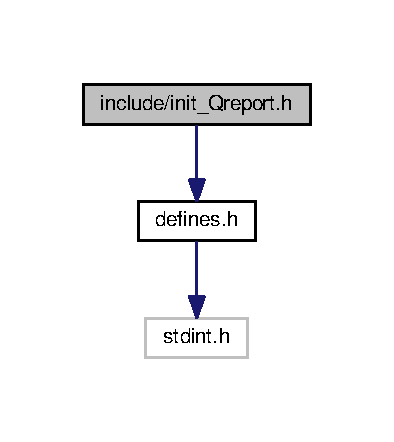
\includegraphics[width=216pt]{init__Qreport_8h__incl}
\end{center}
\end{figure}
This graph shows which files directly or indirectly include this file\+:
\nopagebreak
\begin{figure}[H]
\begin{center}
\leavevmode
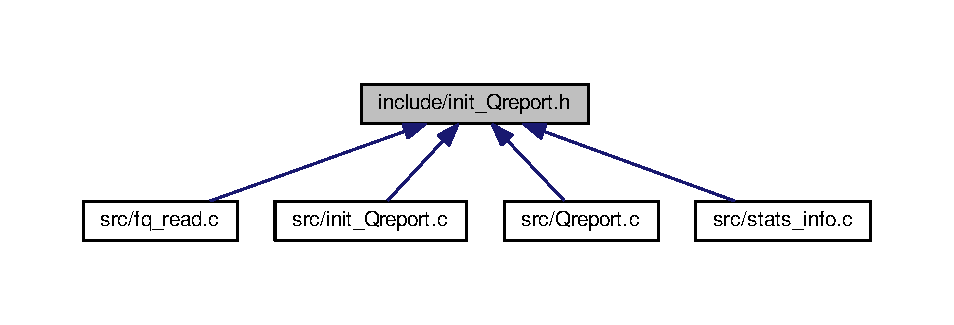
\includegraphics[width=350pt]{init__Qreport_8h__dep__incl}
\end{center}
\end{figure}
\subsection*{Classes}
\begin{DoxyCompactItemize}
\item 
struct \mbox{\hyperlink{struct__iparam__Qreport}{\+\_\+iparam\+\_\+\+Qreport}}
\begin{DoxyCompactList}\small\item\em contains Qreport input parameters \end{DoxyCompactList}\end{DoxyCompactItemize}
\subsection*{Typedefs}
\begin{DoxyCompactItemize}
\item 
\mbox{\Hypertarget{init__Qreport_8h_a883b1b3db368b84ab55f011bbb41bc80}\label{init__Qreport_8h_a883b1b3db368b84ab55f011bbb41bc80}} 
typedef struct \mbox{\hyperlink{struct__iparam__Qreport}{\+\_\+iparam\+\_\+\+Qreport}} \mbox{\hyperlink{init__Qreport_8h_a883b1b3db368b84ab55f011bbb41bc80}{Iparam\+\_\+\+Qreport}}
\begin{DoxyCompactList}\small\item\em contains Qreport input parameters \end{DoxyCompactList}\end{DoxyCompactItemize}
\subsection*{Functions}
\begin{DoxyCompactItemize}
\item 
\mbox{\Hypertarget{init__Qreport_8h_a48be775a109c8bf8672933494d67f30f}\label{init__Qreport_8h_a48be775a109c8bf8672933494d67f30f}} 
void \mbox{\hyperlink{init__Qreport_8h_a48be775a109c8bf8672933494d67f30f}{print\+Help\+Dialog\+\_\+\+Qreport}} ()
\begin{DoxyCompactList}\small\item\em Function that prints Qreport help dialog when called. \end{DoxyCompactList}\item 
\mbox{\Hypertarget{init__Qreport_8h_a0eb2d9339158f29ffe7ae419af56e921}\label{init__Qreport_8h_a0eb2d9339158f29ffe7ae419af56e921}} 
void \mbox{\hyperlink{init__Qreport_8h_a0eb2d9339158f29ffe7ae419af56e921}{getarg\+\_\+\+Qreport}} (int argc, char $\ast$$\ast$argv)
\begin{DoxyCompactList}\small\item\em Reads in the arguments passed through the command line to Qreport. and stores them in the global variable par\+\_\+\+QR. \end{DoxyCompactList}\end{DoxyCompactItemize}


\subsection{Detailed Description}
Header file\+: help dialog for Qreport and initialization of the command line arguments. 

\begin{DoxyAuthor}{Author}
Paula Perez \href{mailto:paulaperezrubio@gmail.com}{\tt paulaperezrubio@gmail.\+com} 
\end{DoxyAuthor}
\begin{DoxyDate}{Date}
03.\+08.\+2017 
\end{DoxyDate}

\hypertarget{Rcommand__Qreport_8h}{}\section{include/\+Rcommand\+\_\+\+Qreport.h File Reference}
\label{Rcommand__Qreport_8h}\index{include/\+Rcommand\+\_\+\+Qreport.\+h@{include/\+Rcommand\+\_\+\+Qreport.\+h}}


get Rscript command for Qreport  


This graph shows which files directly or indirectly include this file\+:
\nopagebreak
\begin{figure}[H]
\begin{center}
\leavevmode
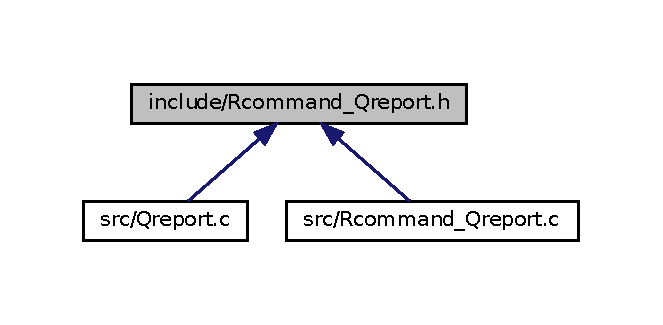
\includegraphics[width=318pt]{Rcommand__Qreport_8h__dep__incl}
\end{center}
\end{figure}
\subsection*{Functions}
\begin{DoxyCompactItemize}
\item 
\mbox{\Hypertarget{Rcommand__Qreport_8h_a336345f346ab2a993022a0ca4862731c}\label{Rcommand__Qreport_8h_a336345f346ab2a993022a0ca4862731c}} 
char $\ast$ \mbox{\hyperlink{Rcommand__Qreport_8h_a336345f346ab2a993022a0ca4862731c}{command\+\_\+\+Qreport}} ()
\begin{DoxyCompactList}\small\item\em returns Rscript command that generates the quality report in html \end{DoxyCompactList}\end{DoxyCompactItemize}


\subsection{Detailed Description}
get Rscript command for Qreport 

\begin{DoxyAuthor}{Author}
Paula Perez \href{mailto:paulaperezrubio@gmail.com}{\tt paulaperezrubio@gmail.\+com} 
\end{DoxyAuthor}
\begin{DoxyDate}{Date}
09.\+08.\+2017 
\end{DoxyDate}

\hypertarget{Rcommand__Sreport_8h}{}\section{include/\+Rcommand\+\_\+\+Sreport.h File Reference}
\label{Rcommand__Sreport_8h}\index{include/\+Rcommand\+\_\+\+Sreport.\+h@{include/\+Rcommand\+\_\+\+Sreport.\+h}}


get Rscript command for Sreport  


This graph shows which files directly or indirectly include this file\+:
\nopagebreak
\begin{figure}[H]
\begin{center}
\leavevmode
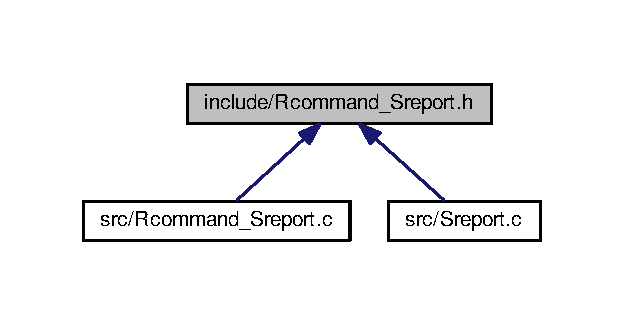
\includegraphics[width=314pt]{Rcommand__Sreport_8h__dep__incl}
\end{center}
\end{figure}
\subsection*{Functions}
\begin{DoxyCompactItemize}
\item 
char $\ast$ \mbox{\hyperlink{Rcommand__Sreport_8h_a843ffc16afb438c7430da804efd8dfaf}{command\+\_\+\+Sreport}} ()
\begin{DoxyCompactList}\small\item\em returns Rscript command that generates the summary report in html \end{DoxyCompactList}\end{DoxyCompactItemize}


\subsection{Detailed Description}
get Rscript command for Sreport 

\begin{DoxyAuthor}{Author}
Paula Perez \href{mailto:paulaperezrubio@gmail.com}{\tt paulaperezrubio@gmail.\+com} 
\end{DoxyAuthor}
\begin{DoxyDate}{Date}
09.\+08.\+2017 
\end{DoxyDate}


\subsection{Function Documentation}
\mbox{\Hypertarget{Rcommand__Sreport_8h_a843ffc16afb438c7430da804efd8dfaf}\label{Rcommand__Sreport_8h_a843ffc16afb438c7430da804efd8dfaf}} 
\index{Rcommand\+\_\+\+Sreport.\+h@{Rcommand\+\_\+\+Sreport.\+h}!command\+\_\+\+Sreport@{command\+\_\+\+Sreport}}
\index{command\+\_\+\+Sreport@{command\+\_\+\+Sreport}!Rcommand\+\_\+\+Sreport.\+h@{Rcommand\+\_\+\+Sreport.\+h}}
\subsubsection{\texorpdfstring{command\+\_\+\+Sreport()}{command\_Sreport()}}
{\footnotesize\ttfamily char$\ast$ command\+\_\+\+Sreport (\begin{DoxyParamCaption}{ }\end{DoxyParamCaption})}



returns Rscript command that generates the summary report in html 


\begin{DoxyCode}
# To run between quotation marks after:  Rscript\_RBioC -e (Rscript)
inputfolder = normalizePath( <par.SR.inputfolder>, mustWork = TRUE);
output = <par\_SR.outputfile>;
output\_file = gsub('.* /', '', output);
path = gsub('[^/]+$', '', output);
if (path != '') \{
  outputfile = paste0(normalizePath(path, mustWork = TRUE), '/', outputfile);
\} else \{
  outputfile = paste0(cwd, '/', output\_file); # cwd: current working dir
\}; 
rmarkdown::render(<par\_SR.Rmd\_file>, 
                  params = list(inputfolder = inputfolder, version= VERSION),
                  output\_file = output\_file)
\end{DoxyCode}
 
\hypertarget{stats__info_8h}{}\section{include/stats\+\_\+info.h File Reference}
\label{stats__info_8h}\index{include/stats\+\_\+info.\+h@{include/stats\+\_\+info.\+h}}


Construct the quality report variables and update them.  


{\ttfamily \#include $<$stdint.\+h$>$}\newline
{\ttfamily \#include $<$stdlib.\+h$>$}\newline
{\ttfamily \#include \char`\"{}fq\+\_\+read.\+h\char`\"{}}\newline
{\ttfamily \#include \char`\"{}defines.\+h\char`\"{}}\newline
Include dependency graph for stats\+\_\+info.\+h\+:
\nopagebreak
\begin{figure}[H]
\begin{center}
\leavevmode
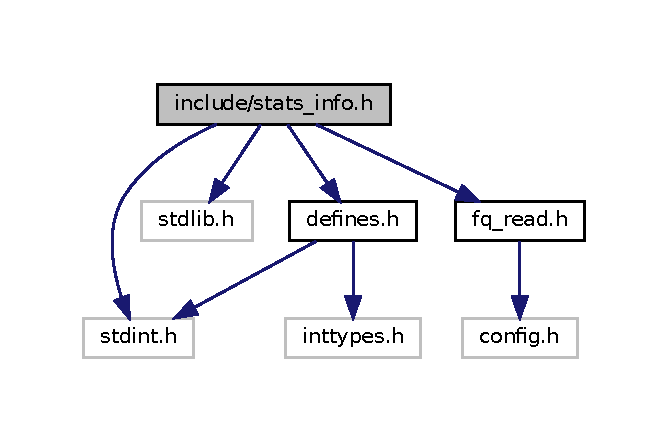
\includegraphics[width=321pt]{stats__info_8h__incl}
\end{center}
\end{figure}
This graph shows which files directly or indirectly include this file\+:
\nopagebreak
\begin{figure}[H]
\begin{center}
\leavevmode
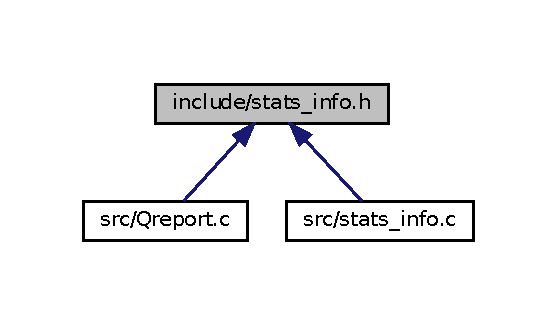
\includegraphics[width=268pt]{stats__info_8h__dep__incl}
\end{center}
\end{figure}
\subsection*{Classes}
\begin{DoxyCompactItemize}
\item 
struct \mbox{\hyperlink{structstatsinfo}{statsinfo}}
\begin{DoxyCompactList}\small\item\em stores info needed to create the summary graphs \end{DoxyCompactList}\end{DoxyCompactItemize}
\subsection*{Typedefs}
\begin{DoxyCompactItemize}
\item 
\mbox{\Hypertarget{stats__info_8h_a2671cb2f7634ad56ed3dc27446796ef1}\label{stats__info_8h_a2671cb2f7634ad56ed3dc27446796ef1}} 
typedef struct \mbox{\hyperlink{structstatsinfo}{statsinfo}} \mbox{\hyperlink{stats__info_8h_a2671cb2f7634ad56ed3dc27446796ef1}{Info}}
\begin{DoxyCompactList}\small\item\em stores info needed to create the summary graphs \end{DoxyCompactList}\end{DoxyCompactItemize}
\subsection*{Functions}
\begin{DoxyCompactItemize}
\item 
void \mbox{\hyperlink{stats__info_8h_a5c125debcca38ba396c6c01ecbc3dd5d}{init\+\_\+info}} (\mbox{\hyperlink{stats__info_8h_a2671cb2f7634ad56ed3dc27446796ef1}{Info}} $\ast$res)
\begin{DoxyCompactList}\small\item\em Initialization of a Info type. \end{DoxyCompactList}\item 
\mbox{\Hypertarget{stats__info_8h_a3354d39b533bb35891251afdb5961a3a}\label{stats__info_8h_a3354d39b533bb35891251afdb5961a3a}} 
void \mbox{\hyperlink{stats__info_8h_a3354d39b533bb35891251afdb5961a3a}{free\+\_\+info}} (\mbox{\hyperlink{stats__info_8h_a2671cb2f7634ad56ed3dc27446796ef1}{Info}} $\ast$res)
\begin{DoxyCompactList}\small\item\em frees allocated memory in Info \end{DoxyCompactList}\item 
\mbox{\Hypertarget{stats__info_8h_a7815bd5c300f89c99b539fa3e4c4f776}\label{stats__info_8h_a7815bd5c300f89c99b539fa3e4c4f776}} 
void \mbox{\hyperlink{stats__info_8h_a7815bd5c300f89c99b539fa3e4c4f776}{read\+\_\+info}} (\mbox{\hyperlink{stats__info_8h_a2671cb2f7634ad56ed3dc27446796ef1}{Info}} $\ast$res, char $\ast$file)
\begin{DoxyCompactList}\small\item\em Read Info from binary file. \end{DoxyCompactList}\item 
\mbox{\Hypertarget{stats__info_8h_ae17b550d0328a66a4941b18f24f2a920}\label{stats__info_8h_ae17b550d0328a66a4941b18f24f2a920}} 
void \mbox{\hyperlink{stats__info_8h_ae17b550d0328a66a4941b18f24f2a920}{write\+\_\+info}} (\mbox{\hyperlink{stats__info_8h_a2671cb2f7634ad56ed3dc27446796ef1}{Info}} $\ast$res, char $\ast$file)
\begin{DoxyCompactList}\small\item\em Write info to binary file. \end{DoxyCompactList}\item 
\mbox{\Hypertarget{stats__info_8h_a76d353cb30ac4cd4bc55362e7359976d}\label{stats__info_8h_a76d353cb30ac4cd4bc55362e7359976d}} 
void \mbox{\hyperlink{stats__info_8h_a76d353cb30ac4cd4bc55362e7359976d}{print\+\_\+info}} (\mbox{\hyperlink{stats__info_8h_a2671cb2f7634ad56ed3dc27446796ef1}{Info}} $\ast$res, char $\ast$infofile)
\begin{DoxyCompactList}\small\item\em print Info to a textfile \end{DoxyCompactList}\item 
\mbox{\Hypertarget{stats__info_8h_a9ca0a2ed2eb78d9a9717b82efcfdcb1f}\label{stats__info_8h_a9ca0a2ed2eb78d9a9717b82efcfdcb1f}} 
void \mbox{\hyperlink{stats__info_8h_a9ca0a2ed2eb78d9a9717b82efcfdcb1f}{get\+\_\+first\+\_\+tile}} (\mbox{\hyperlink{stats__info_8h_a2671cb2f7634ad56ed3dc27446796ef1}{Info}} $\ast$res, \mbox{\hyperlink{fq__read_8h_a9af37aa81397c9531c66863d4e97f034}{Fq\+\_\+read}} $\ast$seq)
\begin{DoxyCompactList}\small\item\em gets first tile \end{DoxyCompactList}\item 
\mbox{\Hypertarget{stats__info_8h_af599aaaf2eb242dcb6e9f44c0eb8c180}\label{stats__info_8h_af599aaaf2eb242dcb6e9f44c0eb8c180}} 
void \mbox{\hyperlink{stats__info_8h_af599aaaf2eb242dcb6e9f44c0eb8c180}{update\+\_\+info}} (\mbox{\hyperlink{stats__info_8h_a2671cb2f7634ad56ed3dc27446796ef1}{Info}} $\ast$res, \mbox{\hyperlink{fq__read_8h_a9af37aa81397c9531c66863d4e97f034}{Fq\+\_\+read}} $\ast$seq)
\begin{DoxyCompactList}\small\item\em updates Info with Fq\+\_\+read \end{DoxyCompactList}\item 
int \mbox{\hyperlink{stats__info_8h_a5bceee4c9ce4858a2e1a1022020f3051}{update\+\_\+\+A\+C\+G\+T\+\_\+counts}} (uint64\+\_\+t $\ast$A\+C\+G\+T\+\_\+low, char A\+C\+GT)
\begin{DoxyCompactList}\small\item\em update, for current tile, A\+C\+GT counts. \end{DoxyCompactList}\item 
\mbox{\Hypertarget{stats__info_8h_a12859b5ec4a85f24df22833b2ddeee79}\label{stats__info_8h_a12859b5ec4a85f24df22833b2ddeee79}} 
void \mbox{\hyperlink{stats__info_8h_a12859b5ec4a85f24df22833b2ddeee79}{update\+\_\+\+Q\+Pos\+Tile\+\_\+table}} (\mbox{\hyperlink{stats__info_8h_a2671cb2f7634ad56ed3dc27446796ef1}{Info}} $\ast$res, \mbox{\hyperlink{fq__read_8h_a9af37aa81397c9531c66863d4e97f034}{Fq\+\_\+read}} $\ast$seq)
\begin{DoxyCompactList}\small\item\em update Q\+Postile table \end{DoxyCompactList}\item 
\mbox{\Hypertarget{stats__info_8h_a89eaadfa007bf08a3d3b5b6dcda9ae37}\label{stats__info_8h_a89eaadfa007bf08a3d3b5b6dcda9ae37}} 
void \mbox{\hyperlink{stats__info_8h_a89eaadfa007bf08a3d3b5b6dcda9ae37}{update\+\_\+\+A\+C\+G\+T\+\_\+pos}} (uint64\+\_\+t $\ast$A\+C\+G\+T\+\_\+pos, \mbox{\hyperlink{fq__read_8h_a9af37aa81397c9531c66863d4e97f034}{Fq\+\_\+read}} $\ast$seq)
\begin{DoxyCompactList}\small\item\em update A\+C\+G\+T\+\_\+pos \end{DoxyCompactList}\item 
void \mbox{\hyperlink{stats__info_8h_a8ca7ce52d36a35e78b8c0bde089aedcf}{resize\+\_\+info}} (\mbox{\hyperlink{stats__info_8h_a2671cb2f7634ad56ed3dc27446796ef1}{Info}} $\ast$res)
\begin{DoxyCompactList}\small\item\em resize Info \end{DoxyCompactList}\end{DoxyCompactItemize}


\subsection{Detailed Description}
Construct the quality report variables and update them. 

\begin{DoxyAuthor}{Author}
Paula Perez \href{mailto:paulaperezrubio@gmail.com}{\tt paulaperezrubio@gmail.\+com} 
\end{DoxyAuthor}
\begin{DoxyDate}{Date}
04.\+08.\+2017 
\end{DoxyDate}


\subsection{Function Documentation}
\mbox{\Hypertarget{stats__info_8h_a5c125debcca38ba396c6c01ecbc3dd5d}\label{stats__info_8h_a5c125debcca38ba396c6c01ecbc3dd5d}} 
\index{stats\+\_\+info.\+h@{stats\+\_\+info.\+h}!init\+\_\+info@{init\+\_\+info}}
\index{init\+\_\+info@{init\+\_\+info}!stats\+\_\+info.\+h@{stats\+\_\+info.\+h}}
\subsubsection{\texorpdfstring{init\+\_\+info()}{init\_info()}}
{\footnotesize\ttfamily void init\+\_\+info (\begin{DoxyParamCaption}\item[{\mbox{\hyperlink{stats__info_8h_a2671cb2f7634ad56ed3dc27446796ef1}{Info}} $\ast$}]{res }\end{DoxyParamCaption})}



Initialization of a Info type. 

It sets\+: nQ, read\+\_\+len, ntiles, minQ and the dimensions of the arrays. Initializes the rest of the variables to zero and allocates memory to the arrays initializing them to 0 (calloc). \mbox{\Hypertarget{stats__info_8h_a8ca7ce52d36a35e78b8c0bde089aedcf}\label{stats__info_8h_a8ca7ce52d36a35e78b8c0bde089aedcf}} 
\index{stats\+\_\+info.\+h@{stats\+\_\+info.\+h}!resize\+\_\+info@{resize\+\_\+info}}
\index{resize\+\_\+info@{resize\+\_\+info}!stats\+\_\+info.\+h@{stats\+\_\+info.\+h}}
\subsubsection{\texorpdfstring{resize\+\_\+info()}{resize\_info()}}
{\footnotesize\ttfamily void resize\+\_\+info (\begin{DoxyParamCaption}\item[{\mbox{\hyperlink{stats__info_8h_a2671cb2f7634ad56ed3dc27446796ef1}{Info}} $\ast$}]{res }\end{DoxyParamCaption})}



resize Info 

At the end of the program, resize the structure Info, and adapt it to the actual number of tiles and the actual number of different quality values present. \mbox{\Hypertarget{stats__info_8h_a5bceee4c9ce4858a2e1a1022020f3051}\label{stats__info_8h_a5bceee4c9ce4858a2e1a1022020f3051}} 
\index{stats\+\_\+info.\+h@{stats\+\_\+info.\+h}!update\+\_\+\+A\+C\+G\+T\+\_\+counts@{update\+\_\+\+A\+C\+G\+T\+\_\+counts}}
\index{update\+\_\+\+A\+C\+G\+T\+\_\+counts@{update\+\_\+\+A\+C\+G\+T\+\_\+counts}!stats\+\_\+info.\+h@{stats\+\_\+info.\+h}}
\subsubsection{\texorpdfstring{update\+\_\+\+A\+C\+G\+T\+\_\+counts()}{update\_ACGT\_counts()}}
{\footnotesize\ttfamily int update\+\_\+\+A\+C\+G\+T\+\_\+counts (\begin{DoxyParamCaption}\item[{uint64\+\_\+t $\ast$}]{A\+C\+G\+T\+\_\+low,  }\item[{char}]{A\+C\+GT }\end{DoxyParamCaption})}



update, for current tile, A\+C\+GT counts. 

Makes update of A\+C\+GT counts for the current tile. Can be used with variables\+: low\+Q\+\_\+\+A\+C\+G\+T\+\_\+tile and A\+C\+G\+T\+\_\+tile 
\hypertarget{str__manip_8h}{\section{include/str\+\_\+manip.h File Reference}
\label{str__manip_8h}\index{include/str\+\_\+manip.\+h@{include/str\+\_\+manip.\+h}}
}


functions that do string manipulation  


This graph shows which files directly or indirectly include this file\+:\nopagebreak
\begin{figure}[H]
\begin{center}
\leavevmode
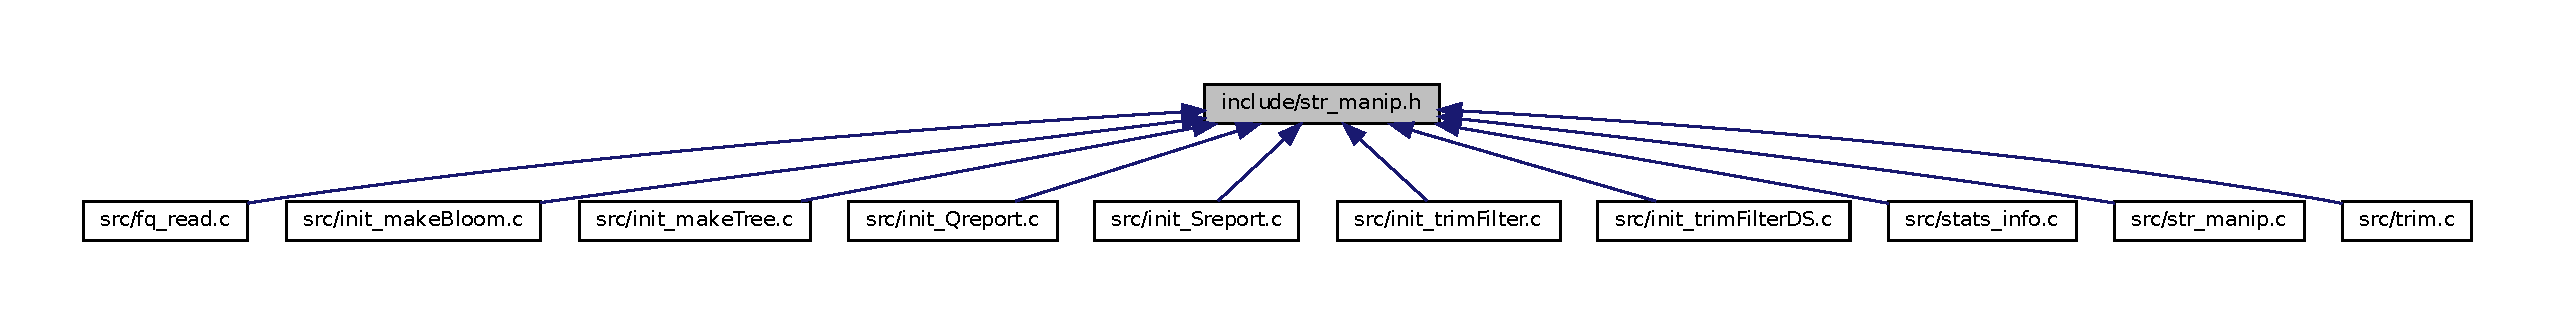
\includegraphics[width=350pt]{str__manip_8h__dep__incl}
\end{center}
\end{figure}
\subsection*{Classes}
\begin{DoxyCompactItemize}
\item 
struct \hyperlink{struct__split}{\+\_\+split}
\begin{DoxyCompactList}\small\item\em contains a splitted string and the number or splitted fields \end{DoxyCompactList}\end{DoxyCompactItemize}
\subsection*{Typedefs}
\begin{DoxyCompactItemize}
\item 
\hypertarget{str__manip_8h_aeff63a40ce3fff0c51bd207baeba2013}{typedef struct \hyperlink{struct__split}{\+\_\+split} \hyperlink{str__manip_8h_aeff63a40ce3fff0c51bd207baeba2013}{Split}}\label{str__manip_8h_aeff63a40ce3fff0c51bd207baeba2013}

\begin{DoxyCompactList}\small\item\em contains a splitted string and the number or splitted fields \end{DoxyCompactList}\end{DoxyCompactItemize}
\subsection*{Functions}
\begin{DoxyCompactItemize}
\item 
\hypertarget{str__manip_8h_a15e8cbc96aa4cea159dbc59d1c01ffaa}{int \hyperlink{str__manip_8h_a15e8cbc96aa4cea159dbc59d1c01ffaa}{str\+\_\+isascii} (char $\ast$s)}\label{str__manip_8h_a15e8cbc96aa4cea159dbc59d1c01ffaa}

\begin{DoxyCompactList}\small\item\em return nonzero iff all elements in the string are in the A\+S\+C\+I\+I set. \end{DoxyCompactList}\item 
int \hyperlink{str__manip_8h_a8108ab52dfbc1af644bf7682c1bbe33f}{strindex} (char $\ast$s, char $\ast$t)
\begin{DoxyCompactList}\small\item\em returns index of t in s (start, first occurence) \end{DoxyCompactList}\item 
\hypertarget{str__manip_8h_af8d13ec7edfe3ca8a03f48bd7e3b1d83}{int \hyperlink{str__manip_8h_af8d13ec7edfe3ca8a03f48bd7e3b1d83}{count\+\_\+char} (char $\ast$s, char c)}\label{str__manip_8h_af8d13ec7edfe3ca8a03f48bd7e3b1d83}

\begin{DoxyCompactList}\small\item\em returns the \# of occurences of char c in string s \end{DoxyCompactList}\item 
\hyperlink{str__manip_8h_aeff63a40ce3fff0c51bd207baeba2013}{Split} \hyperlink{str__manip_8h_a245675aede3b8bedd8ce6c8c2aa70ec0}{strsplit} (char $\ast$str, char sep)
\begin{DoxyCompactList}\small\item\em Separates strings by a separator. \end{DoxyCompactList}\end{DoxyCompactItemize}


\subsection{Detailed Description}
functions that do string manipulation 

\begin{DoxyAuthor}{Author}
Paula Perez \href{mailto:paulaperezrubio@gmail.com}{\tt paulaperezrubio@gmail.\+com} 
\end{DoxyAuthor}
\begin{DoxyDate}{Date}
03.\+08.\+2017 
\end{DoxyDate}


\subsection{Function Documentation}
\hypertarget{str__manip_8h_a8108ab52dfbc1af644bf7682c1bbe33f}{\index{str\+\_\+manip.\+h@{str\+\_\+manip.\+h}!strindex@{strindex}}
\index{strindex@{strindex}!str\+\_\+manip.\+h@{str\+\_\+manip.\+h}}
\subsubsection[{strindex}]{\setlength{\rightskip}{0pt plus 5cm}int strindex (
\begin{DoxyParamCaption}
\item[{char $\ast$}]{s, }
\item[{char $\ast$}]{t}
\end{DoxyParamCaption}
)}}\label{str__manip_8h_a8108ab52dfbc1af644bf7682c1bbe33f}


returns index of t in s (start, first occurence) 


\begin{DoxyParams}{Parameters}
{\em s} & string to be checked. \\
\hline
{\em t} & substring to be found in s. \\
\hline
\end{DoxyParams}
\hypertarget{str__manip_8h_a245675aede3b8bedd8ce6c8c2aa70ec0}{\index{str\+\_\+manip.\+h@{str\+\_\+manip.\+h}!strsplit@{strsplit}}
\index{strsplit@{strsplit}!str\+\_\+manip.\+h@{str\+\_\+manip.\+h}}
\subsubsection[{strsplit}]{\setlength{\rightskip}{0pt plus 5cm}{\bf Split} strsplit (
\begin{DoxyParamCaption}
\item[{char $\ast$}]{str, }
\item[{char}]{sep}
\end{DoxyParamCaption}
)}}\label{str__manip_8h_a245675aede3b8bedd8ce6c8c2aa70ec0}


Separates strings by a separator. 


\begin{DoxyParams}{Parameters}
{\em str} & input string \\
\hline
{\em sep} & separator (char) \\
\hline
\end{DoxyParams}
\begin{DoxyReturn}{Returns}
array of strings containing the substrings in the input separated 
\end{DoxyReturn}

\hypertarget{fopen__gen_8c}{}\section{src/fopen\+\_\+gen.c File Reference}
\label{fopen__gen_8c}\index{src/fopen\+\_\+gen.\+c@{src/fopen\+\_\+gen.\+c}}


Uncompress/compress input/output files using pipes.  


{\ttfamily \#include $<$stdlib.\+h$>$}\newline
{\ttfamily \#include $<$string.\+h$>$}\newline
{\ttfamily \#include $<$unistd.\+h$>$}\newline
{\ttfamily \#include $<$assert.\+h$>$}\newline
{\ttfamily \#include $<$sys/types.\+h$>$}\newline
{\ttfamily \#include $<$fcntl.\+h$>$}\newline
{\ttfamily \#include \char`\"{}fopen\+\_\+gen.\+h\char`\"{}}\newline
Include dependency graph for fopen\+\_\+gen.\+c\+:
\nopagebreak
\begin{figure}[H]
\begin{center}
\leavevmode
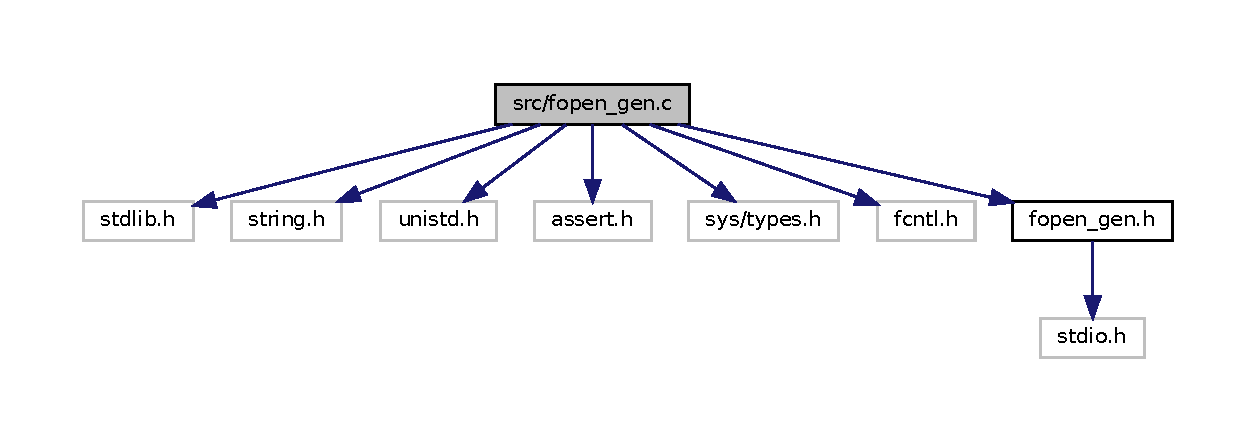
\includegraphics[width=350pt]{fopen__gen_8c__incl}
\end{center}
\end{figure}
\subsection*{Functions}
\begin{DoxyCompactItemize}
\item 
\mbox{\Hypertarget{fopen__gen_8c_a103afa931e1ef96c23ac490151b64036}\label{fopen__gen_8c_a103afa931e1ef96c23ac490151b64036}} 
static const char $\ast$ {\bfseries zcat\+Exec} (const char $\ast$path)
\item 
\mbox{\Hypertarget{fopen__gen_8c_aaad17dde0a82955fa873b2a8b93c99ae}\label{fopen__gen_8c_aaad17dde0a82955fa873b2a8b93c99ae}} 
static const char $\ast$ \mbox{\hyperlink{fopen__gen_8c_aaad17dde0a82955fa873b2a8b93c99ae}{cat\+Exec}} (const char $\ast$path)
\begin{DoxyCompactList}\small\item\em Commands to compress files. To be done in output. \end{DoxyCompactList}\item 
static int \mbox{\hyperlink{fopen__gen_8c_ad91f7120fe65477ca4ccc599808434e6}{uncompress}} (const char $\ast$path)
\begin{DoxyCompactList}\small\item\em Open a pipe to uncompress file. Open a pipe to uncompress the specified file. Not thread safe. \end{DoxyCompactList}\item 
static int \mbox{\hyperlink{fopen__gen_8c_a1d546df97e4f524a9a23e4e5bb92cff9}{compress}} (const char $\ast$path)
\begin{DoxyCompactList}\small\item\em Open a pipe to compress output. Open a pipe to uncompress the specified file. Not thread safe. \end{DoxyCompactList}\item 
\mbox{\Hypertarget{fopen__gen_8c_ae59755703d84f781f127762acf2deb6d}\label{fopen__gen_8c_ae59755703d84f781f127762acf2deb6d}} 
int {\bfseries set\+Cloexec} (int fd)
\item 
static F\+I\+LE $\ast$ \mbox{\hyperlink{fopen__gen_8c_a97fe7a7fd381b9f81e4adbdeab902766}{funcompress}} (const char $\ast$path)
\begin{DoxyCompactList}\small\item\em Open a pipe to uncompress the specified file. \end{DoxyCompactList}\item 
static F\+I\+LE $\ast$ \mbox{\hyperlink{fopen__gen_8c_a86f9e75b840d00dce91e44cf880f730d}{fcompress}} (const char $\ast$path)
\begin{DoxyCompactList}\small\item\em Open a pipe to compress the specified file. \end{DoxyCompactList}\item 
F\+I\+LE $\ast$ \mbox{\hyperlink{fopen__gen_8c_ae03fc1b9180f740dcb577fdb00072fb3}{fopen\+\_\+gen}} (const char $\ast$path, const char $\ast$mode)
\begin{DoxyCompactList}\small\item\em Generalized fopen function. fopen\+\_\+gen is to be used as fopen. Can be used in read and in write mode. When used in read mode with a compressed extension, the file will be first decompressed and then read. When used in write mode with a compressed extension, the output will be compressed. \end{DoxyCompactList}\end{DoxyCompactItemize}


\subsection{Detailed Description}
Uncompress/compress input/output files using pipes. 

Hook the standard file opening functions, open, fopen and fopen64. If the extension of the file being opened indicates the file is compressed (.gz, .bz2, .xz), when opening in the reading mode a pipe to a program is opened that decompresses that file (gunzip, bunzip2 or xzdec) and return a handle to the open pipe. When opening in the writing mode (only for .gz, .bam), a pipe to a program is opened that compresses the output.

\begin{DoxyAuthor}{Author}
Paula Perez \href{mailto:paulaperezrubio@gmail.com}{\tt paulaperezrubio@gmail.\+com} 
\end{DoxyAuthor}
\begin{DoxyDate}{Date}
03.\+08.\+2017 
\end{DoxyDate}
\begin{DoxyWarning}{Warning}
vfork vs fork to be checked! 
\end{DoxyWarning}
\begin{DoxyNote}{Note}
-\/ original copyright note -\/ (reading mode, original C++ code) author\+: Shaun Jackman \href{mailto:sjackman@bcgsc.ca}{\tt sjackman@bcgsc.\+ca}, \href{https://github.com/bcgsc,}{\tt https\+://github.\+com/bcgsc,} ~\newline
filename\+: Uncompress.\+cpp 
\end{DoxyNote}


\subsection{Function Documentation}
\mbox{\Hypertarget{fopen__gen_8c_a1d546df97e4f524a9a23e4e5bb92cff9}\label{fopen__gen_8c_a1d546df97e4f524a9a23e4e5bb92cff9}} 
\index{fopen\+\_\+gen.\+c@{fopen\+\_\+gen.\+c}!compress@{compress}}
\index{compress@{compress}!fopen\+\_\+gen.\+c@{fopen\+\_\+gen.\+c}}
\subsubsection{\texorpdfstring{compress()}{compress()}}
{\footnotesize\ttfamily static int compress (\begin{DoxyParamCaption}\item[{const char $\ast$}]{path }\end{DoxyParamCaption})\hspace{0.3cm}{\ttfamily [static]}}



Open a pipe to compress output. Open a pipe to uncompress the specified file. Not thread safe. 

\begin{DoxyReturn}{Returns}
a file descriptor 
\end{DoxyReturn}
\mbox{\Hypertarget{fopen__gen_8c_a86f9e75b840d00dce91e44cf880f730d}\label{fopen__gen_8c_a86f9e75b840d00dce91e44cf880f730d}} 
\index{fopen\+\_\+gen.\+c@{fopen\+\_\+gen.\+c}!fcompress@{fcompress}}
\index{fcompress@{fcompress}!fopen\+\_\+gen.\+c@{fopen\+\_\+gen.\+c}}
\subsubsection{\texorpdfstring{fcompress()}{fcompress()}}
{\footnotesize\ttfamily static F\+I\+LE$\ast$ fcompress (\begin{DoxyParamCaption}\item[{const char $\ast$}]{path }\end{DoxyParamCaption})\hspace{0.3cm}{\ttfamily [static]}}



Open a pipe to compress the specified file. 

\begin{DoxyReturn}{Returns}
a F\+I\+LE pointer 
\end{DoxyReturn}
\mbox{\Hypertarget{fopen__gen_8c_ae03fc1b9180f740dcb577fdb00072fb3}\label{fopen__gen_8c_ae03fc1b9180f740dcb577fdb00072fb3}} 
\index{fopen\+\_\+gen.\+c@{fopen\+\_\+gen.\+c}!fopen\+\_\+gen@{fopen\+\_\+gen}}
\index{fopen\+\_\+gen@{fopen\+\_\+gen}!fopen\+\_\+gen.\+c@{fopen\+\_\+gen.\+c}}
\subsubsection{\texorpdfstring{fopen\+\_\+gen()}{fopen\_gen()}}
{\footnotesize\ttfamily F\+I\+LE$\ast$ fopen\+\_\+gen (\begin{DoxyParamCaption}\item[{const char $\ast$}]{path,  }\item[{const char $\ast$}]{mode }\end{DoxyParamCaption})}



Generalized fopen function. fopen\+\_\+gen is to be used as fopen. Can be used in read and in write mode. When used in read mode with a compressed extension, the file will be first decompressed and then read. When used in write mode with a compressed extension, the output will be compressed. 

\begin{DoxyReturn}{Returns}
a F\+I\+LE pointer 
\end{DoxyReturn}
\mbox{\Hypertarget{fopen__gen_8c_a97fe7a7fd381b9f81e4adbdeab902766}\label{fopen__gen_8c_a97fe7a7fd381b9f81e4adbdeab902766}} 
\index{fopen\+\_\+gen.\+c@{fopen\+\_\+gen.\+c}!funcompress@{funcompress}}
\index{funcompress@{funcompress}!fopen\+\_\+gen.\+c@{fopen\+\_\+gen.\+c}}
\subsubsection{\texorpdfstring{funcompress()}{funcompress()}}
{\footnotesize\ttfamily static F\+I\+LE$\ast$ funcompress (\begin{DoxyParamCaption}\item[{const char $\ast$}]{path }\end{DoxyParamCaption})\hspace{0.3cm}{\ttfamily [static]}}



Open a pipe to uncompress the specified file. 

\begin{DoxyReturn}{Returns}
a F\+I\+LE pointer 
\end{DoxyReturn}
\mbox{\Hypertarget{fopen__gen_8c_ad91f7120fe65477ca4ccc599808434e6}\label{fopen__gen_8c_ad91f7120fe65477ca4ccc599808434e6}} 
\index{fopen\+\_\+gen.\+c@{fopen\+\_\+gen.\+c}!uncompress@{uncompress}}
\index{uncompress@{uncompress}!fopen\+\_\+gen.\+c@{fopen\+\_\+gen.\+c}}
\subsubsection{\texorpdfstring{uncompress()}{uncompress()}}
{\footnotesize\ttfamily static int uncompress (\begin{DoxyParamCaption}\item[{const char $\ast$}]{path }\end{DoxyParamCaption})\hspace{0.3cm}{\ttfamily [static]}}



Open a pipe to uncompress file. Open a pipe to uncompress the specified file. Not thread safe. 

\begin{DoxyReturn}{Returns}
a file descriptor 
\end{DoxyReturn}

\hypertarget{fq__read_8c}{\section{src/fq\+\_\+read.c File Reference}
\label{fq__read_8c}\index{src/fq\+\_\+read.\+c@{src/fq\+\_\+read.\+c}}
}


fastq entries manipulations (read/write)  


{\ttfamily \#include $<$string.\+h$>$}\\*
{\ttfamily \#include $<$stdio.\+h$>$}\\*
{\ttfamily \#include $<$stdlib.\+h$>$}\\*
{\ttfamily \#include \char`\"{}init\+\_\+\+Qreport.\+h\char`\"{}}\\*
{\ttfamily \#include \char`\"{}fq\+\_\+read.\+h\char`\"{}}\\*
{\ttfamily \#include \char`\"{}str\+\_\+manip.\+h\char`\"{}}\\*
Include dependency graph for fq\+\_\+read.\+c\+:\nopagebreak
\begin{figure}[H]
\begin{center}
\leavevmode
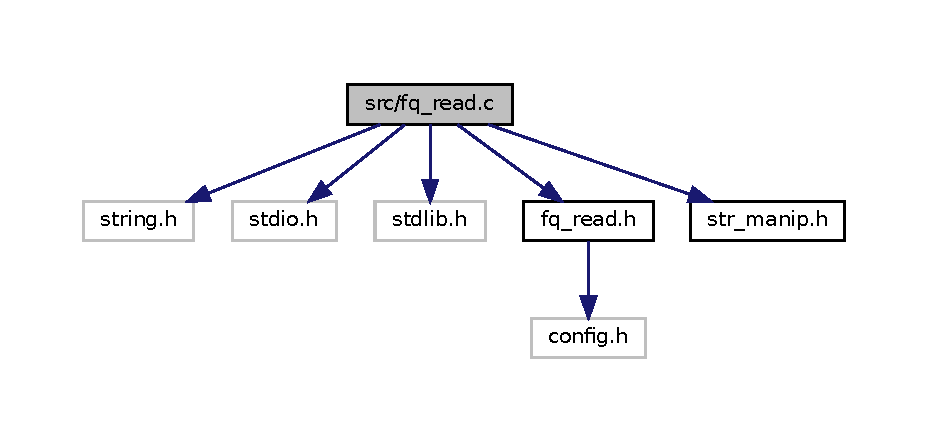
\includegraphics[width=350pt]{fq__read_8c__incl}
\end{center}
\end{figure}
\subsection*{Functions}
\begin{DoxyCompactItemize}
\item 
void \hyperlink{fq__read_8c_a65766fec27771b0b42524625f76d067b}{get\+\_\+fqread} (\hyperlink{fq__read_8h_a9af37aa81397c9531c66863d4e97f034}{Fq\+\_\+read} $\ast$seq, char $\ast$buffer, int pos1, int pos2, int nline)
\begin{DoxyCompactList}\small\item\em reads fastq line from a buffer \end{DoxyCompactList}\item 
int \hyperlink{fq__read_8c_ae58e185777143cd1fc4c75fccd5c647a}{string\+\_\+seq} (\hyperlink{fq__read_8h_a9af37aa81397c9531c66863d4e97f034}{Fq\+\_\+read} $\ast$seq, char $\ast$char\+\_\+seq)
\begin{DoxyCompactList}\small\item\em writes the fq entry in a string \end{DoxyCompactList}\end{DoxyCompactItemize}
\subsection*{Variables}
\begin{DoxyCompactItemize}
\item 
\hyperlink{init__Qreport_8h_a883b1b3db368b84ab55f011bbb41bc80}{Iparam\+\_\+\+Qreport} \hyperlink{fq__read_8c_a5c6527d396580d559cfd1916fc959e23}{par\+\_\+\+Q\+R}
\end{DoxyCompactItemize}


\subsection{Detailed Description}
fastq entries manipulations (read/write) 

\begin{DoxyAuthor}{Author}
Paula Perez \href{mailto:paulaperezrubio@gmail.com}{\tt paulaperezrubio@gmail.\+com} 
\end{DoxyAuthor}
\begin{DoxyDate}{Date}
03.\+08.\+2017 
\end{DoxyDate}


\subsection{Function Documentation}
\hypertarget{fq__read_8c_a65766fec27771b0b42524625f76d067b}{\index{fq\+\_\+read.\+c@{fq\+\_\+read.\+c}!get\+\_\+fqread@{get\+\_\+fqread}}
\index{get\+\_\+fqread@{get\+\_\+fqread}!fq\+\_\+read.\+c@{fq\+\_\+read.\+c}}
\subsubsection[{get\+\_\+fqread}]{\setlength{\rightskip}{0pt plus 5cm}void get\+\_\+fqread (
\begin{DoxyParamCaption}
\item[{{\bf Fq\+\_\+read} $\ast$}]{seq, }
\item[{char $\ast$}]{buffer, }
\item[{int}]{pos1, }
\item[{int}]{pos2, }
\item[{int}]{nline}
\end{DoxyParamCaption}
)}}\label{fq__read_8c_a65766fec27771b0b42524625f76d067b}


reads fastq line from a buffer 

a fastq line is read from a buffer and the relevant information is stored in a structure {\bfseries Fq\+\_\+read}. Depending on the variable {\bfseries par\+\_\+\+Q\+R} values, information about whether the read was trimmed is stored.


\begin{DoxyParams}{Parameters}
{\em $\ast$seq} & pointer to {\bfseries Fq\+\_\+read}, where the info will be stored. \\
\hline
{\em buffer} & variable where the file being read is stored. \\
\hline
{\em pos1} & buffer start position of the line. \\
\hline
{\em pos2} & buffer end position of the line. \\
\hline
{\em nline} & file line number being read. \\
\hline
\end{DoxyParams}
\hypertarget{fq__read_8c_ae58e185777143cd1fc4c75fccd5c647a}{\index{fq\+\_\+read.\+c@{fq\+\_\+read.\+c}!string\+\_\+seq@{string\+\_\+seq}}
\index{string\+\_\+seq@{string\+\_\+seq}!fq\+\_\+read.\+c@{fq\+\_\+read.\+c}}
\subsubsection[{string\+\_\+seq}]{\setlength{\rightskip}{0pt plus 5cm}int string\+\_\+seq (
\begin{DoxyParamCaption}
\item[{{\bf Fq\+\_\+read} $\ast$}]{seq, }
\item[{char $\ast$}]{char\+\_\+seq}
\end{DoxyParamCaption}
)}}\label{fq__read_8c_ae58e185777143cd1fc4c75fccd5c647a}


writes the fq entry in a string 


\begin{DoxyParams}{Parameters}
{\em $\ast$seq} & pointer to {\bfseries Fq\+\_\+read}, where the info will be stored. \\
\hline
{\em char\+\_\+seq} & pointer to buffer, where the sequence will be stored \\
\hline
\end{DoxyParams}
\begin{DoxyWarning}{Warning}
change the call to sprintf to snprintf 
\end{DoxyWarning}


\subsection{Variable Documentation}
\hypertarget{fq__read_8c_a5c6527d396580d559cfd1916fc959e23}{\index{fq\+\_\+read.\+c@{fq\+\_\+read.\+c}!par\+\_\+\+Q\+R@{par\+\_\+\+Q\+R}}
\index{par\+\_\+\+Q\+R@{par\+\_\+\+Q\+R}!fq\+\_\+read.\+c@{fq\+\_\+read.\+c}}
\subsubsection[{par\+\_\+\+Q\+R}]{\setlength{\rightskip}{0pt plus 5cm}{\bf Iparam\+\_\+\+Qreport} par\+\_\+\+Q\+R}}\label{fq__read_8c_a5c6527d396580d559cfd1916fc959e23}
input parameters

global variable\+: input parameters for Qreport 
\hypertarget{init__Qreport_8c}{\section{src/init\+\_\+\+Qreport.c File Reference}
\label{init__Qreport_8c}\index{src/init\+\_\+\+Qreport.\+c@{src/init\+\_\+\+Qreport.\+c}}
}


Help dialog for Qreport and initialization of the command line arguments.  


{\ttfamily \#include $<$getopt.\+h$>$}\\*
{\ttfamily \#include $<$stdio.\+h$>$}\\*
{\ttfamily \#include $<$string.\+h$>$}\\*
{\ttfamily \#include $<$stdlib.\+h$>$}\\*
{\ttfamily \#include \char`\"{}init\+\_\+\+Qreport.\+h\char`\"{}}\\*
{\ttfamily \#include \char`\"{}config.\+h\char`\"{}}\\*
{\ttfamily \#include \char`\"{}defines.\+h\char`\"{}}\\*
Include dependency graph for init\+\_\+\+Qreport.\+c\+:\nopagebreak
\begin{figure}[H]
\begin{center}
\leavevmode
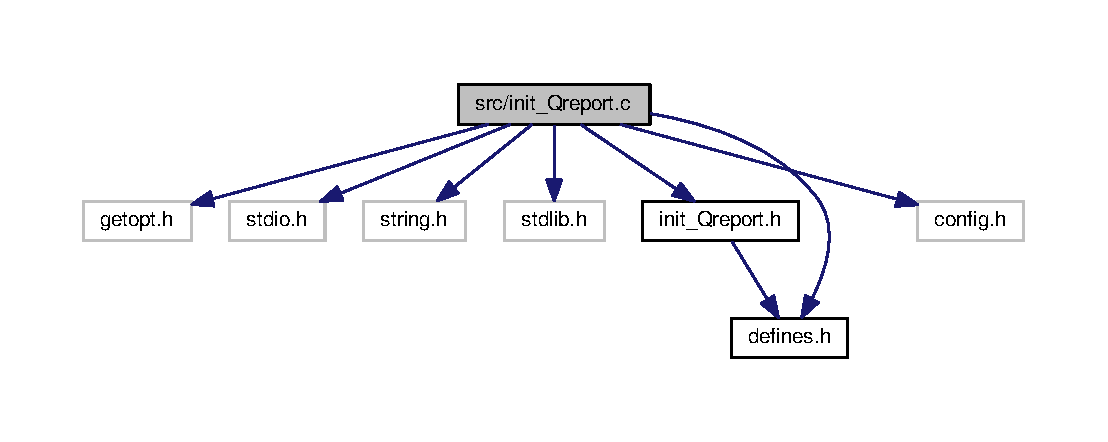
\includegraphics[width=350pt]{init__Qreport_8c__incl}
\end{center}
\end{figure}
\subsection*{Functions}
\begin{DoxyCompactItemize}
\item 
\hypertarget{init__Qreport_8c_a48be775a109c8bf8672933494d67f30f}{void \hyperlink{init__Qreport_8c_a48be775a109c8bf8672933494d67f30f}{print\+Help\+Dialog\+\_\+\+Qreport} ()}\label{init__Qreport_8c_a48be775a109c8bf8672933494d67f30f}

\begin{DoxyCompactList}\small\item\em Function that prints Qreport help dialog when called. \end{DoxyCompactList}\item 
\hypertarget{init__Qreport_8c_a0eb2d9339158f29ffe7ae419af56e921}{void \hyperlink{init__Qreport_8c_a0eb2d9339158f29ffe7ae419af56e921}{getarg\+\_\+\+Qreport} (int argc, char $\ast$$\ast$argv)}\label{init__Qreport_8c_a0eb2d9339158f29ffe7ae419af56e921}

\begin{DoxyCompactList}\small\item\em Reads in the arguments passed through the command line to Qreport. and stores them in the global variable par\+\_\+\+Q\+R. \end{DoxyCompactList}\end{DoxyCompactItemize}
\subsection*{Variables}
\begin{DoxyCompactItemize}
\item 
\hyperlink{init__Qreport_8h_a883b1b3db368b84ab55f011bbb41bc80}{Iparam\+\_\+\+Qreport} \hyperlink{init__Qreport_8c_a5c6527d396580d559cfd1916fc959e23}{par\+\_\+\+Q\+R}
\end{DoxyCompactItemize}


\subsection{Detailed Description}
Help dialog for Qreport and initialization of the command line arguments. 

\begin{DoxyAuthor}{Author}
Paula Perez \href{mailto:paulaperezrubio@gmail.com}{\tt paulaperezrubio@gmail.\+com} 
\end{DoxyAuthor}
\begin{DoxyDate}{Date}
03.\+08.\+2017 
\end{DoxyDate}


\subsection{Variable Documentation}
\hypertarget{init__Qreport_8c_a5c6527d396580d559cfd1916fc959e23}{\index{init\+\_\+\+Qreport.\+c@{init\+\_\+\+Qreport.\+c}!par\+\_\+\+Q\+R@{par\+\_\+\+Q\+R}}
\index{par\+\_\+\+Q\+R@{par\+\_\+\+Q\+R}!init\+\_\+\+Qreport.\+c@{init\+\_\+\+Qreport.\+c}}
\subsubsection[{par\+\_\+\+Q\+R}]{\setlength{\rightskip}{0pt plus 5cm}{\bf Iparam\+\_\+\+Qreport} par\+\_\+\+Q\+R}}\label{init__Qreport_8c_a5c6527d396580d559cfd1916fc959e23}
input parameters

global variable\+: input parameters 
\hypertarget{init__Sreport_8c}{}\section{src/init\+\_\+\+Sreport.c File Reference}
\label{init__Sreport_8c}\index{src/init\+\_\+\+Sreport.\+c@{src/init\+\_\+\+Sreport.\+c}}


Help dialog for Sreport and initialization of the command line arguments.  


{\ttfamily \#include $<$getopt.\+h$>$}\newline
{\ttfamily \#include $<$stdio.\+h$>$}\newline
{\ttfamily \#include $<$stdlib.\+h$>$}\newline
{\ttfamily \#include $<$string.\+h$>$}\newline
{\ttfamily \#include \char`\"{}str\+\_\+manip.\+h\char`\"{}}\newline
{\ttfamily \#include \char`\"{}init\+\_\+\+Sreport.\+h\char`\"{}}\newline
{\ttfamily \#include \char`\"{}config.\+h\char`\"{}}\newline
Include dependency graph for init\+\_\+\+Sreport.\+c\+:
\nopagebreak
\begin{figure}[H]
\begin{center}
\leavevmode
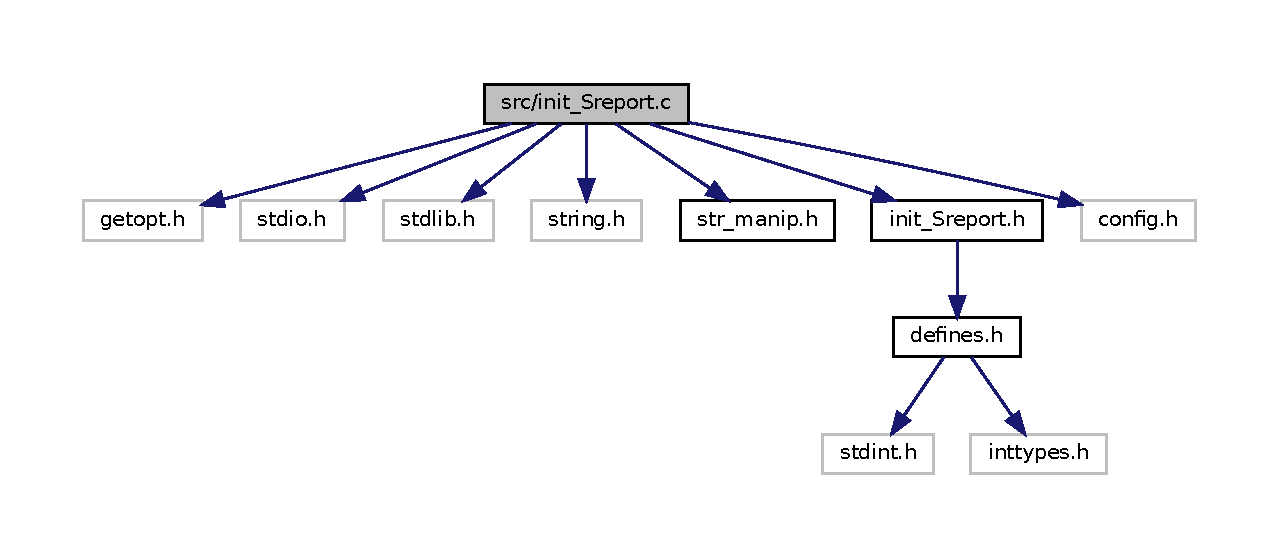
\includegraphics[width=350pt]{init__Sreport_8c__incl}
\end{center}
\end{figure}
\subsection*{Functions}
\begin{DoxyCompactItemize}
\item 
\mbox{\Hypertarget{init__Sreport_8c_a80638b0730feac5c7634c29c6f08ee9e}\label{init__Sreport_8c_a80638b0730feac5c7634c29c6f08ee9e}} 
void \mbox{\hyperlink{init__Sreport_8c_a80638b0730feac5c7634c29c6f08ee9e}{print\+Help\+Dialog\+\_\+\+Sreport}} ()
\begin{DoxyCompactList}\small\item\em Function that prints Sreport help dialog when called. \end{DoxyCompactList}\item 
\mbox{\Hypertarget{init__Sreport_8c_a5a266a01d36227a9094c023aed7a1e8c}\label{init__Sreport_8c_a5a266a01d36227a9094c023aed7a1e8c}} 
void \mbox{\hyperlink{init__Sreport_8c_a5a266a01d36227a9094c023aed7a1e8c}{getarg\+\_\+\+Sreport}} (int argc, char $\ast$$\ast$argv)
\begin{DoxyCompactList}\small\item\em Reads in the arguments passed through the command line to Sreport. and stores them in the global variable par\+\_\+\+SR. \end{DoxyCompactList}\end{DoxyCompactItemize}
\subsection*{Variables}
\begin{DoxyCompactItemize}
\item 
\mbox{\hyperlink{init__Sreport_8h_ae7c35fd710a54db5b21f5c6b04fe9a5d}{Iparam\+\_\+\+Sreport}} \mbox{\hyperlink{init__Sreport_8c_aa230276b7e03d43430c998def780682e}{par\+\_\+\+SR}}
\end{DoxyCompactItemize}


\subsection{Detailed Description}
Help dialog for Sreport and initialization of the command line arguments. 

\begin{DoxyAuthor}{Author}
Paula Perez \href{mailto:paulaperezrubio@gmail.com}{\tt paulaperezrubio@gmail.\+com} 
\end{DoxyAuthor}
\begin{DoxyDate}{Date}
09.\+08.\+2017 
\end{DoxyDate}


\subsection{Variable Documentation}
\mbox{\Hypertarget{init__Sreport_8c_aa230276b7e03d43430c998def780682e}\label{init__Sreport_8c_aa230276b7e03d43430c998def780682e}} 
\index{init\+\_\+\+Sreport.\+c@{init\+\_\+\+Sreport.\+c}!par\+\_\+\+SR@{par\+\_\+\+SR}}
\index{par\+\_\+\+SR@{par\+\_\+\+SR}!init\+\_\+\+Sreport.\+c@{init\+\_\+\+Sreport.\+c}}
\subsubsection{\texorpdfstring{par\+\_\+\+SR}{par\_SR}}
{\footnotesize\ttfamily \mbox{\hyperlink{init__Sreport_8h_ae7c35fd710a54db5b21f5c6b04fe9a5d}{Iparam\+\_\+\+Sreport}} par\+\_\+\+SR}

input parameters Sreport 
\hypertarget{Qreport_8c}{\section{src/\+Qreport.c File Reference}
\label{Qreport_8c}\index{src/\+Qreport.\+c@{src/\+Qreport.\+c}}
}


Q\+Report main function.  


{\ttfamily \#include $<$stdio.\+h$>$}\\*
{\ttfamily \#include $<$stdlib.\+h$>$}\\*
{\ttfamily \#include $<$string.\+h$>$}\\*
{\ttfamily \#include $<$time.\+h$>$}\\*
{\ttfamily \#include \char`\"{}init\+\_\+\+Qreport.\+h\char`\"{}}\\*
{\ttfamily \#include \char`\"{}fopen\+\_\+gen.\+h\char`\"{}}\\*
{\ttfamily \#include \char`\"{}fq\+\_\+read.\+h\char`\"{}}\\*
{\ttfamily \#include \char`\"{}stats\+\_\+info.\+h\char`\"{}}\\*
{\ttfamily \#include \char`\"{}Rcommand\+\_\+\+Qreport.\+h\char`\"{}}\\*
Include dependency graph for Qreport.\+c\+:
\nopagebreak
\begin{figure}[H]
\begin{center}
\leavevmode
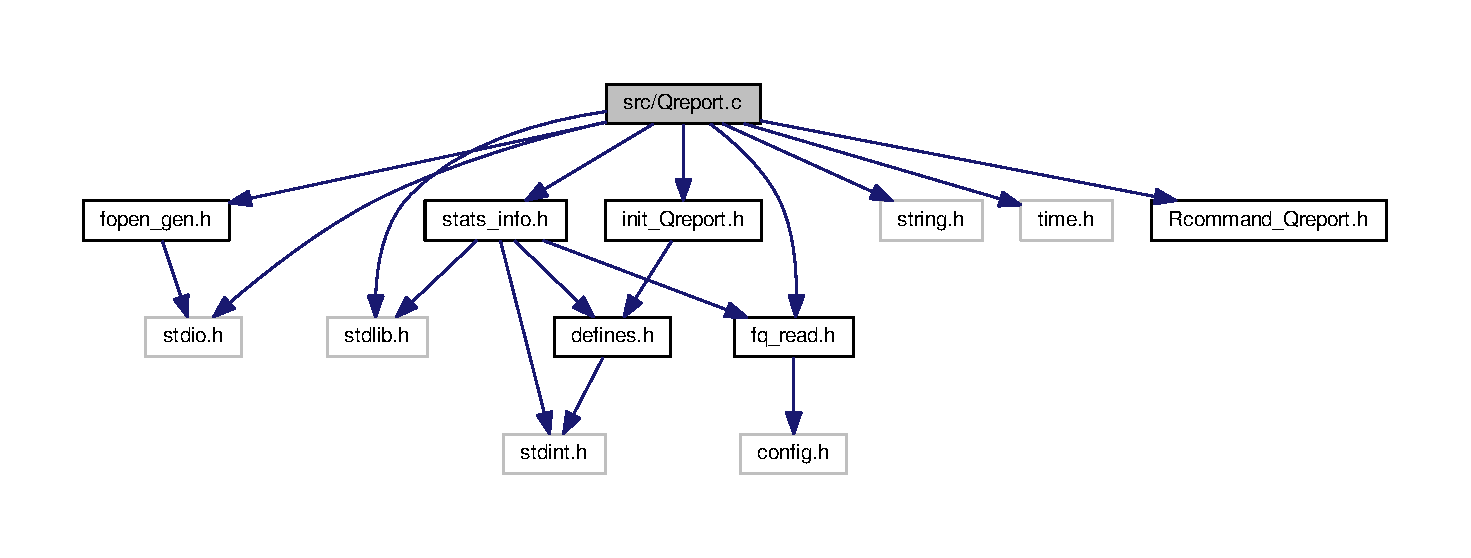
\includegraphics[width=350pt]{Qreport_8c__incl}
\end{center}
\end{figure}
\subsection*{Macros}
\begin{DoxyCompactItemize}
\item 
\#define \hyperlink{Qreport_8c_a4419cb9bb22330d00cfd4727a05060dd}{B\+\_\+\+L\+E\+N}~131072
\end{DoxyCompactItemize}
\subsection*{Functions}
\begin{DoxyCompactItemize}
\item 
\hypertarget{Qreport_8c_a0ddf1224851353fc92bfbff6f499fa97}{int \hyperlink{Qreport_8c_a0ddf1224851353fc92bfbff6f499fa97}{main} (int argc, char $\ast$argv\mbox{[}$\,$\mbox{]})}\label{Qreport_8c_a0ddf1224851353fc92bfbff6f499fa97}

\begin{DoxyCompactList}\small\item\em Qreport main function. \end{DoxyCompactList}\end{DoxyCompactItemize}
\subsection*{Variables}
\begin{DoxyCompactItemize}
\item 
\hyperlink{init__Qreport_8h_a883b1b3db368b84ab55f011bbb41bc80}{Iparam\+\_\+\+Qreport} \hyperlink{Qreport_8c_a5c6527d396580d559cfd1916fc959e23}{par\+\_\+\+Q\+R}
\end{DoxyCompactItemize}


\subsection{Detailed Description}
Q\+Report main function. 

\begin{DoxyAuthor}{Author}
Paula Perez \href{mailto:paulaperezrubio@gmail.com}{\tt paulaperezrubio@gmail.\+com} 
\end{DoxyAuthor}
\begin{DoxyDate}{Date}
03.\+08.\+2017 This file contains the quality report main function. It reads a fastq file and creates a html quality report. See R\+E\+A\+D\+M\+E\+\_\+\+Qreport.\+md for more details. 
\end{DoxyDate}


\subsection{Macro Definition Documentation}
\hypertarget{Qreport_8c_a4419cb9bb22330d00cfd4727a05060dd}{\index{Qreport.\+c@{Qreport.\+c}!B\+\_\+\+L\+E\+N@{B\+\_\+\+L\+E\+N}}
\index{B\+\_\+\+L\+E\+N@{B\+\_\+\+L\+E\+N}!Qreport.\+c@{Qreport.\+c}}
\subsubsection[{B\+\_\+\+L\+E\+N}]{\setlength{\rightskip}{0pt plus 5cm}\#define B\+\_\+\+L\+E\+N~131072}}\label{Qreport_8c_a4419cb9bb22330d00cfd4727a05060dd}
buffer size 

\subsection{Variable Documentation}
\hypertarget{Qreport_8c_a5c6527d396580d559cfd1916fc959e23}{\index{Qreport.\+c@{Qreport.\+c}!par\+\_\+\+Q\+R@{par\+\_\+\+Q\+R}}
\index{par\+\_\+\+Q\+R@{par\+\_\+\+Q\+R}!Qreport.\+c@{Qreport.\+c}}
\subsubsection[{par\+\_\+\+Q\+R}]{\setlength{\rightskip}{0pt plus 5cm}{\bf Iparam\+\_\+\+Qreport} par\+\_\+\+Q\+R}}\label{Qreport_8c_a5c6527d396580d559cfd1916fc959e23}
global variable\+: input parameters 
\hypertarget{Rcommand__Sreport_8c}{}\section{src/\+Rcommand\+\_\+\+Sreport.c File Reference}
\label{Rcommand__Sreport_8c}\index{src/\+Rcommand\+\_\+\+Sreport.\+c@{src/\+Rcommand\+\_\+\+Sreport.\+c}}


get Rscript command for Sreport  


{\ttfamily \#include $<$stdio.\+h$>$}\newline
{\ttfamily \#include $<$stdlib.\+h$>$}\newline
{\ttfamily \#include $<$unistd.\+h$>$}\newline
{\ttfamily \#include \char`\"{}Rcommand\+\_\+\+Sreport.\+h\char`\"{}}\newline
{\ttfamily \#include \char`\"{}init\+\_\+\+Sreport.\+h\char`\"{}}\newline
{\ttfamily \#include \char`\"{}defines.\+h\char`\"{}}\newline
{\ttfamily \#include \char`\"{}config.\+h\char`\"{}}\newline
Include dependency graph for Rcommand\+\_\+\+Sreport.\+c\+:
\nopagebreak
\begin{figure}[H]
\begin{center}
\leavevmode
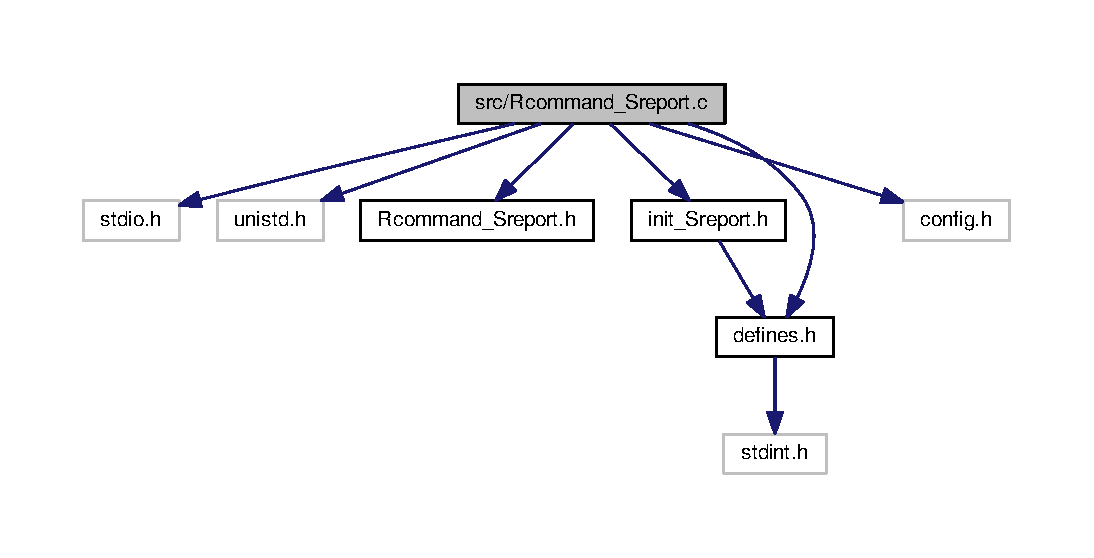
\includegraphics[width=350pt]{Rcommand__Sreport_8c__incl}
\end{center}
\end{figure}
\subsection*{Functions}
\begin{DoxyCompactItemize}
\item 
char $\ast$ \mbox{\hyperlink{Rcommand__Sreport_8c_a843ffc16afb438c7430da804efd8dfaf}{command\+\_\+\+Sreport}} ()
\begin{DoxyCompactList}\small\item\em returns Rscript command that generates the summary report in html \end{DoxyCompactList}\end{DoxyCompactItemize}
\subsection*{Variables}
\begin{DoxyCompactItemize}
\item 
\mbox{\hyperlink{init__Sreport_8h_ae7c35fd710a54db5b21f5c6b04fe9a5d}{Iparam\+\_\+\+Sreport}} \mbox{\hyperlink{Rcommand__Sreport_8c_aa230276b7e03d43430c998def780682e}{par\+\_\+\+SR}}
\end{DoxyCompactItemize}


\subsection{Detailed Description}
get Rscript command for Sreport 

\begin{DoxyAuthor}{Author}
Paula Perez \href{mailto:paulaperezrubio@gmail.com}{\tt paulaperezrubio@gmail.\+com} 
\end{DoxyAuthor}
\begin{DoxyDate}{Date}
09.\+08.\+2017 
\end{DoxyDate}


\subsection{Function Documentation}
\mbox{\Hypertarget{Rcommand__Sreport_8c_a843ffc16afb438c7430da804efd8dfaf}\label{Rcommand__Sreport_8c_a843ffc16afb438c7430da804efd8dfaf}} 
\index{Rcommand\+\_\+\+Sreport.\+c@{Rcommand\+\_\+\+Sreport.\+c}!command\+\_\+\+Sreport@{command\+\_\+\+Sreport}}
\index{command\+\_\+\+Sreport@{command\+\_\+\+Sreport}!Rcommand\+\_\+\+Sreport.\+c@{Rcommand\+\_\+\+Sreport.\+c}}
\subsubsection{\texorpdfstring{command\+\_\+\+Sreport()}{command\_Sreport()}}
{\footnotesize\ttfamily char$\ast$ command\+\_\+\+Sreport (\begin{DoxyParamCaption}{ }\end{DoxyParamCaption})}



returns Rscript command that generates the summary report in html 


\begin{DoxyCode}
# To run between quotation marks after:  Rscript\_RBioC -e (Rscript)
inputfolder = normalizePath( <par.SR.inputfolder>, mustWork = TRUE);
output = <par\_SR.outputfile>;
output\_file = gsub('.* /', '', output);
path = gsub('[^/]+$', '', output);
if (path != '') \{
  outputfile = paste0(normalizePath(path, mustWork = TRUE), '/', outputfile);
\} else \{
  outputfile = paste0(cwd, '/', output\_file); # cwd: current working dir
\}; 
rmarkdown::render(<par\_SR.Rmd\_file>, 
                  params = list(inputfolder = inputfolder, version= VERSION),
                  output\_file = output\_file)
\end{DoxyCode}
 

\subsection{Variable Documentation}
\mbox{\Hypertarget{Rcommand__Sreport_8c_aa230276b7e03d43430c998def780682e}\label{Rcommand__Sreport_8c_aa230276b7e03d43430c998def780682e}} 
\index{Rcommand\+\_\+\+Sreport.\+c@{Rcommand\+\_\+\+Sreport.\+c}!par\+\_\+\+SR@{par\+\_\+\+SR}}
\index{par\+\_\+\+SR@{par\+\_\+\+SR}!Rcommand\+\_\+\+Sreport.\+c@{Rcommand\+\_\+\+Sreport.\+c}}
\subsubsection{\texorpdfstring{par\+\_\+\+SR}{par\_SR}}
{\footnotesize\ttfamily \mbox{\hyperlink{init__Sreport_8h_ae7c35fd710a54db5b21f5c6b04fe9a5d}{Iparam\+\_\+\+Sreport}} par\+\_\+\+SR}

input parameters Sreport 
\hypertarget{Sreport_8c}{\section{src/\+Sreport.c File Reference}
\label{Sreport_8c}\index{src/\+Sreport.\+c@{src/\+Sreport.\+c}}
}


Sreport main function.  


{\ttfamily \#include $<$stdio.\+h$>$}\\*
{\ttfamily \#include $<$stdlib.\+h$>$}\\*
{\ttfamily \#include $<$time.\+h$>$}\\*
{\ttfamily \#include \char`\"{}init\+\_\+\+Sreport.\+h\char`\"{}}\\*
{\ttfamily \#include \char`\"{}Rcommand\+\_\+\+Sreport.\+h\char`\"{}}\\*
{\ttfamily \#include \char`\"{}config.\+h\char`\"{}}\\*
Include dependency graph for Sreport.\+c\+:\nopagebreak
\begin{figure}[H]
\begin{center}
\leavevmode
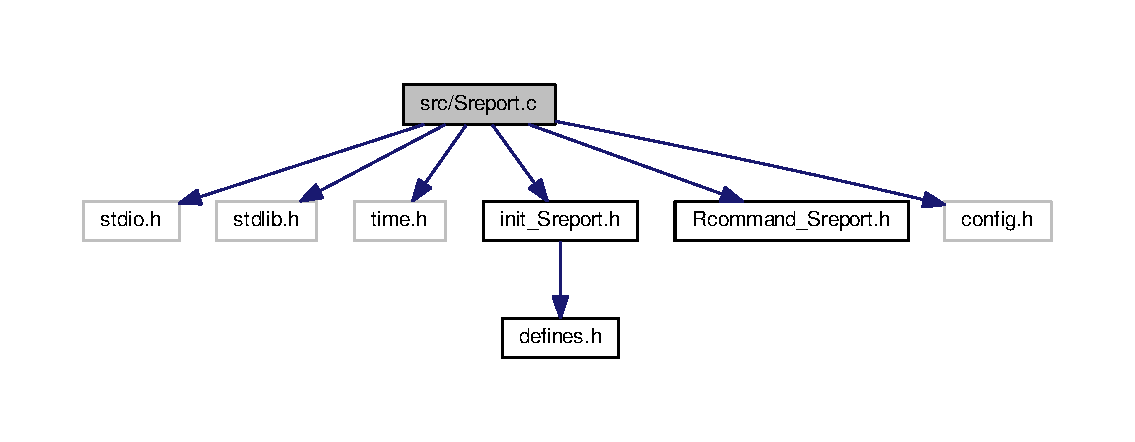
\includegraphics[width=350pt]{Sreport_8c__incl}
\end{center}
\end{figure}
\subsection*{Functions}
\begin{DoxyCompactItemize}
\item 
\hypertarget{Sreport_8c_a0ddf1224851353fc92bfbff6f499fa97}{int \hyperlink{Sreport_8c_a0ddf1224851353fc92bfbff6f499fa97}{main} (int argc, char $\ast$argv\mbox{[}$\,$\mbox{]})}\label{Sreport_8c_a0ddf1224851353fc92bfbff6f499fa97}

\begin{DoxyCompactList}\small\item\em Qreport main function. \end{DoxyCompactList}\end{DoxyCompactItemize}
\subsection*{Variables}
\begin{DoxyCompactItemize}
\item 
\hyperlink{init__Sreport_8h_ae7c35fd710a54db5b21f5c6b04fe9a5d}{Iparam\+\_\+\+Sreport} \hyperlink{Sreport_8c_aa230276b7e03d43430c998def780682e}{par\+\_\+\+S\+R}
\end{DoxyCompactItemize}


\subsection{Detailed Description}
Sreport main function. 

\begin{DoxyAuthor}{Author}
Paula Perez \href{mailto:paulaperezrubio@gmail.com}{\tt paulaperezrubio@gmail.\+com} 
\end{DoxyAuthor}
\begin{DoxyDate}{Date}
09.\+08.\+2017 This file contains the summary report main function. Given a folder containing $\ast$bin as from Qreport output, Sreport generates a summary report in html format. See R\+E\+A\+D\+M\+E\+\_\+\+Sreport.\+md for more details. 
\end{DoxyDate}


\subsection{Variable Documentation}
\hypertarget{Sreport_8c_aa230276b7e03d43430c998def780682e}{\index{Sreport.\+c@{Sreport.\+c}!par\+\_\+\+S\+R@{par\+\_\+\+S\+R}}
\index{par\+\_\+\+S\+R@{par\+\_\+\+S\+R}!Sreport.\+c@{Sreport.\+c}}
\subsubsection[{par\+\_\+\+S\+R}]{\setlength{\rightskip}{0pt plus 5cm}{\bf Iparam\+\_\+\+Sreport} par\+\_\+\+S\+R}}\label{Sreport_8c_aa230276b7e03d43430c998def780682e}
input parameters Sreport 
\hypertarget{stats__info_8c}{\section{src/stats\+\_\+info.c File Reference}
\label{stats__info_8c}\index{src/stats\+\_\+info.\+c@{src/stats\+\_\+info.\+c}}
}


Construct the quality report variables and update them.  


{\ttfamily \#include $<$stdio.\+h$>$}\\*
{\ttfamily \#include $<$string.\+h$>$}\\*
{\ttfamily \#include \char`\"{}stats\+\_\+info.\+h\char`\"{}}\\*
{\ttfamily \#include \char`\"{}init\+\_\+\+Qreport.\+h\char`\"{}}\\*
{\ttfamily \#include \char`\"{}str\+\_\+manip.\+h\char`\"{}}\\*
Include dependency graph for stats\+\_\+info.\+c\+:\nopagebreak
\begin{figure}[H]
\begin{center}
\leavevmode
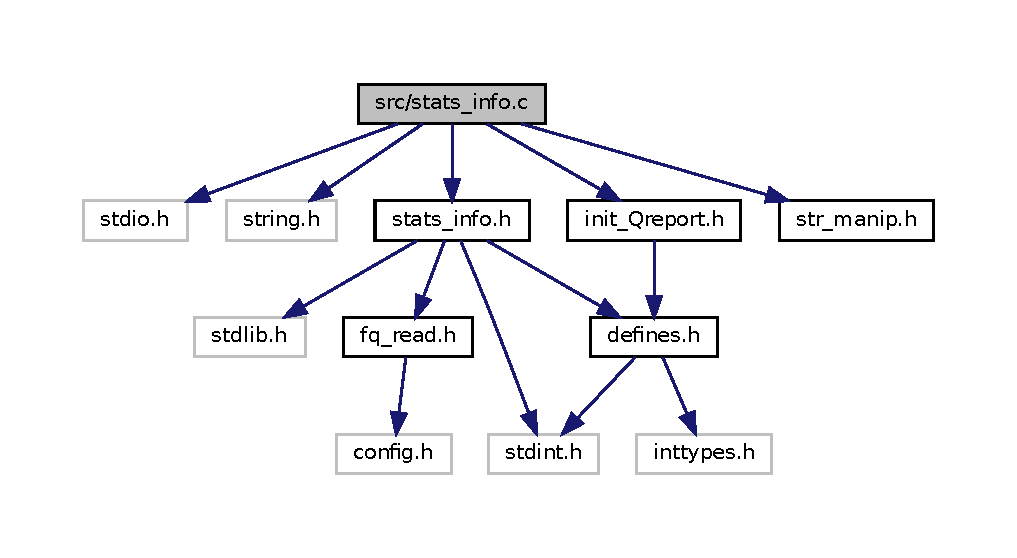
\includegraphics[width=350pt]{stats__info_8c__incl}
\end{center}
\end{figure}
\subsection*{Functions}
\begin{DoxyCompactItemize}
\item 
void \hyperlink{stats__info_8c_a5475bae263602449a0bb1af3ea112ad3}{get\+\_\+tile\+\_\+lane} (char $\ast$line1, int $\ast$tile, int $\ast$lane)
\begin{DoxyCompactList}\small\item\em get tile number from first line in fastq entry. \end{DoxyCompactList}\item 
\hypertarget{stats__info_8c_a398c4dad447f1384af6d620500788a0a}{static int \hyperlink{stats__info_8c_a398c4dad447f1384af6d620500788a0a}{belongsto} (int k, int $\ast$qual\+\_\+tags, int n\+Q)}\label{stats__info_8c_a398c4dad447f1384af6d620500788a0a}

\begin{DoxyCompactList}\small\item\em returns 1 if k is in qual\+\_\+tags, 0 otherwise. \end{DoxyCompactList}\item 
\hypertarget{stats__info_8c_ac4b64efac6b92ff63774c58b92d0fdb5}{static int \hyperlink{stats__info_8c_ac4b64efac6b92ff63774c58b92d0fdb5}{cmpfunc} (const void $\ast$a, const void $\ast$b)}\label{stats__info_8c_ac4b64efac6b92ff63774c58b92d0fdb5}

\begin{DoxyCompactList}\small\item\em comparison function for qsort \end{DoxyCompactList}\item 
void \hyperlink{stats__info_8c_a5c125debcca38ba396c6c01ecbc3dd5d}{init\+\_\+info} (\hyperlink{stats__info_8h_a2671cb2f7634ad56ed3dc27446796ef1}{Info} $\ast$res)
\begin{DoxyCompactList}\small\item\em Initialization of a Info type. \end{DoxyCompactList}\item 
\hypertarget{stats__info_8c_a3354d39b533bb35891251afdb5961a3a}{void \hyperlink{stats__info_8c_a3354d39b533bb35891251afdb5961a3a}{free\+\_\+info} (\hyperlink{stats__info_8h_a2671cb2f7634ad56ed3dc27446796ef1}{Info} $\ast$res)}\label{stats__info_8c_a3354d39b533bb35891251afdb5961a3a}

\begin{DoxyCompactList}\small\item\em frees allocated memory in Info \end{DoxyCompactList}\item 
\hypertarget{stats__info_8c_a7815bd5c300f89c99b539fa3e4c4f776}{void \hyperlink{stats__info_8c_a7815bd5c300f89c99b539fa3e4c4f776}{read\+\_\+info} (\hyperlink{stats__info_8h_a2671cb2f7634ad56ed3dc27446796ef1}{Info} $\ast$res, char $\ast$file)}\label{stats__info_8c_a7815bd5c300f89c99b539fa3e4c4f776}

\begin{DoxyCompactList}\small\item\em Read Info from binary file. \end{DoxyCompactList}\item 
\hypertarget{stats__info_8c_ae17b550d0328a66a4941b18f24f2a920}{void \hyperlink{stats__info_8c_ae17b550d0328a66a4941b18f24f2a920}{write\+\_\+info} (\hyperlink{stats__info_8h_a2671cb2f7634ad56ed3dc27446796ef1}{Info} $\ast$res, char $\ast$file)}\label{stats__info_8c_ae17b550d0328a66a4941b18f24f2a920}

\begin{DoxyCompactList}\small\item\em Write info to binary file. \end{DoxyCompactList}\item 
\hypertarget{stats__info_8c_a76d353cb30ac4cd4bc55362e7359976d}{void \hyperlink{stats__info_8c_a76d353cb30ac4cd4bc55362e7359976d}{print\+\_\+info} (\hyperlink{stats__info_8h_a2671cb2f7634ad56ed3dc27446796ef1}{Info} $\ast$res, char $\ast$infofile)}\label{stats__info_8c_a76d353cb30ac4cd4bc55362e7359976d}

\begin{DoxyCompactList}\small\item\em print Info to a textfile \end{DoxyCompactList}\item 
\hypertarget{stats__info_8c_a9ca0a2ed2eb78d9a9717b82efcfdcb1f}{void \hyperlink{stats__info_8c_a9ca0a2ed2eb78d9a9717b82efcfdcb1f}{get\+\_\+first\+\_\+tile} (\hyperlink{stats__info_8h_a2671cb2f7634ad56ed3dc27446796ef1}{Info} $\ast$res, \hyperlink{fq__read_8h_a9af37aa81397c9531c66863d4e97f034}{Fq\+\_\+read} $\ast$seq)}\label{stats__info_8c_a9ca0a2ed2eb78d9a9717b82efcfdcb1f}

\begin{DoxyCompactList}\small\item\em gets first tile \end{DoxyCompactList}\item 
\hypertarget{stats__info_8c_af599aaaf2eb242dcb6e9f44c0eb8c180}{void \hyperlink{stats__info_8c_af599aaaf2eb242dcb6e9f44c0eb8c180}{update\+\_\+info} (\hyperlink{stats__info_8h_a2671cb2f7634ad56ed3dc27446796ef1}{Info} $\ast$res, \hyperlink{fq__read_8h_a9af37aa81397c9531c66863d4e97f034}{Fq\+\_\+read} $\ast$seq)}\label{stats__info_8c_af599aaaf2eb242dcb6e9f44c0eb8c180}

\begin{DoxyCompactList}\small\item\em updates Info with Fq\+\_\+read \end{DoxyCompactList}\item 
int \hyperlink{stats__info_8c_a5bceee4c9ce4858a2e1a1022020f3051}{update\+\_\+\+A\+C\+G\+T\+\_\+counts} (uint64\+\_\+t $\ast$A\+C\+G\+T\+\_\+low, char A\+C\+G\+T)
\begin{DoxyCompactList}\small\item\em update, for current tile, A\+C\+G\+T counts. \end{DoxyCompactList}\item 
\hypertarget{stats__info_8c_a12859b5ec4a85f24df22833b2ddeee79}{void \hyperlink{stats__info_8c_a12859b5ec4a85f24df22833b2ddeee79}{update\+\_\+\+Q\+Pos\+Tile\+\_\+table} (\hyperlink{stats__info_8h_a2671cb2f7634ad56ed3dc27446796ef1}{Info} $\ast$res, \hyperlink{fq__read_8h_a9af37aa81397c9531c66863d4e97f034}{Fq\+\_\+read} $\ast$seq)}\label{stats__info_8c_a12859b5ec4a85f24df22833b2ddeee79}

\begin{DoxyCompactList}\small\item\em update Q\+Postile table \end{DoxyCompactList}\item 
\hypertarget{stats__info_8c_a0bf1e9e20a67a78adc88e500610b45f7}{void \hyperlink{stats__info_8c_a0bf1e9e20a67a78adc88e500610b45f7}{update\+\_\+\+A\+C\+G\+T\+\_\+pos} (uint64\+\_\+t $\ast$A\+C\+G\+T\+\_\+pos, \hyperlink{fq__read_8h_a9af37aa81397c9531c66863d4e97f034}{Fq\+\_\+read} $\ast$seq, int read\+\_\+len)}\label{stats__info_8c_a0bf1e9e20a67a78adc88e500610b45f7}

\begin{DoxyCompactList}\small\item\em update A\+C\+G\+T\+\_\+pos \end{DoxyCompactList}\item 
void \hyperlink{stats__info_8c_a8ca7ce52d36a35e78b8c0bde089aedcf}{resize\+\_\+info} (\hyperlink{stats__info_8h_a2671cb2f7634ad56ed3dc27446796ef1}{Info} $\ast$res)
\begin{DoxyCompactList}\small\item\em resize Info \end{DoxyCompactList}\end{DoxyCompactItemize}
\subsection*{Variables}
\begin{DoxyCompactItemize}
\item 
\hyperlink{init__Qreport_8h_a883b1b3db368b84ab55f011bbb41bc80}{Iparam\+\_\+\+Qreport} \hyperlink{stats__info_8c_a5c6527d396580d559cfd1916fc959e23}{par\+\_\+\+Q\+R}
\end{DoxyCompactItemize}


\subsection{Detailed Description}
Construct the quality report variables and update them. 

\begin{DoxyAuthor}{Author}
Paula Perez \href{mailto:paulaperezrubio@gmail.com}{\tt paulaperezrubio@gmail.\+com} 
\end{DoxyAuthor}
\begin{DoxyDate}{Date}
04.\+08.\+2017 
\end{DoxyDate}


\subsection{Function Documentation}
\hypertarget{stats__info_8c_a5475bae263602449a0bb1af3ea112ad3}{\index{stats\+\_\+info.\+c@{stats\+\_\+info.\+c}!get\+\_\+tile\+\_\+lane@{get\+\_\+tile\+\_\+lane}}
\index{get\+\_\+tile\+\_\+lane@{get\+\_\+tile\+\_\+lane}!stats\+\_\+info.\+c@{stats\+\_\+info.\+c}}
\subsubsection[{get\+\_\+tile\+\_\+lane}]{\setlength{\rightskip}{0pt plus 5cm}void get\+\_\+tile\+\_\+lane (
\begin{DoxyParamCaption}
\item[{char $\ast$}]{line1, }
\item[{int $\ast$}]{tile, }
\item[{int $\ast$}]{lane}
\end{DoxyParamCaption}
)}}\label{stats__info_8c_a5475bae263602449a0bb1af3ea112ad3}


get tile number from first line in fastq entry. 


\begin{DoxyParams}{Parameters}
{\em line1} & first line of a fastq entry \\
\hline
{\em tile} & int$\ast$ where the tile will be stored \\
\hline
{\em lane} & int$\ast$ where the lane will be stored \\
\hline
\end{DoxyParams}
\begin{DoxySeeAlso}{See also}
\href{http://wiki.christophchamp.com/index.php?title=FASTQ_format}{\tt http\+://wiki.\+christophchamp.\+com/index.\+php?title=\+F\+A\+S\+T\+Q\+\_\+format}
\end{DoxySeeAlso}
Only Illumina sequence identifiers are allowed. The line is inspected, and the number of '\+:' is obtained. The function exits with an error if the number of semicolons is different from 4 or 9. \hypertarget{stats__info_8c_a5c125debcca38ba396c6c01ecbc3dd5d}{\index{stats\+\_\+info.\+c@{stats\+\_\+info.\+c}!init\+\_\+info@{init\+\_\+info}}
\index{init\+\_\+info@{init\+\_\+info}!stats\+\_\+info.\+c@{stats\+\_\+info.\+c}}
\subsubsection[{init\+\_\+info}]{\setlength{\rightskip}{0pt plus 5cm}void init\+\_\+info (
\begin{DoxyParamCaption}
\item[{{\bf Info} $\ast$}]{res}
\end{DoxyParamCaption}
)}}\label{stats__info_8c_a5c125debcca38ba396c6c01ecbc3dd5d}


Initialization of a Info type. 

It sets\+: n\+Q, read\+\_\+len, ntiles, min\+Q and the dimensions of the arrays. Initializes the rest of the variables to zero and allocates memory to the arrays initializing them to 0 (calloc). \hypertarget{stats__info_8c_a8ca7ce52d36a35e78b8c0bde089aedcf}{\index{stats\+\_\+info.\+c@{stats\+\_\+info.\+c}!resize\+\_\+info@{resize\+\_\+info}}
\index{resize\+\_\+info@{resize\+\_\+info}!stats\+\_\+info.\+c@{stats\+\_\+info.\+c}}
\subsubsection[{resize\+\_\+info}]{\setlength{\rightskip}{0pt plus 5cm}void resize\+\_\+info (
\begin{DoxyParamCaption}
\item[{{\bf Info} $\ast$}]{res}
\end{DoxyParamCaption}
)}}\label{stats__info_8c_a8ca7ce52d36a35e78b8c0bde089aedcf}


resize Info 

At the end of the program, resize the structure Info, and adapt it to the actual number of tiles and the actual number of different quality values present. \hypertarget{stats__info_8c_a5bceee4c9ce4858a2e1a1022020f3051}{\index{stats\+\_\+info.\+c@{stats\+\_\+info.\+c}!update\+\_\+\+A\+C\+G\+T\+\_\+counts@{update\+\_\+\+A\+C\+G\+T\+\_\+counts}}
\index{update\+\_\+\+A\+C\+G\+T\+\_\+counts@{update\+\_\+\+A\+C\+G\+T\+\_\+counts}!stats\+\_\+info.\+c@{stats\+\_\+info.\+c}}
\subsubsection[{update\+\_\+\+A\+C\+G\+T\+\_\+counts}]{\setlength{\rightskip}{0pt plus 5cm}int update\+\_\+\+A\+C\+G\+T\+\_\+counts (
\begin{DoxyParamCaption}
\item[{uint64\+\_\+t $\ast$}]{A\+C\+G\+T\+\_\+low, }
\item[{char}]{A\+C\+G\+T}
\end{DoxyParamCaption}
)}}\label{stats__info_8c_a5bceee4c9ce4858a2e1a1022020f3051}


update, for current tile, A\+C\+G\+T counts. 

Makes update of A\+C\+G\+T counts for the current tile. Can be used with variables\+: low\+Q\+\_\+\+A\+C\+G\+T\+\_\+tile and A\+C\+G\+T\+\_\+tile 

\subsection{Variable Documentation}
\hypertarget{stats__info_8c_a5c6527d396580d559cfd1916fc959e23}{\index{stats\+\_\+info.\+c@{stats\+\_\+info.\+c}!par\+\_\+\+Q\+R@{par\+\_\+\+Q\+R}}
\index{par\+\_\+\+Q\+R@{par\+\_\+\+Q\+R}!stats\+\_\+info.\+c@{stats\+\_\+info.\+c}}
\subsubsection[{par\+\_\+\+Q\+R}]{\setlength{\rightskip}{0pt plus 5cm}{\bf Iparam\+\_\+\+Qreport} par\+\_\+\+Q\+R}}\label{stats__info_8c_a5c6527d396580d559cfd1916fc959e23}
global variable\+: input parameters for Qreport 
\hypertarget{str__manip_8c}{\section{src/str\+\_\+manip.c File Reference}
\label{str__manip_8c}\index{src/str\+\_\+manip.\+c@{src/str\+\_\+manip.\+c}}
}


functions that do string manipulation  


{\ttfamily \#include $<$stdio.\+h$>$}\\*
{\ttfamily \#include $<$stdlib.\+h$>$}\\*
{\ttfamily \#include $<$string.\+h$>$}\\*
{\ttfamily \#include \char`\"{}str\+\_\+manip.\+h\char`\"{}}\\*
Include dependency graph for str\+\_\+manip.\+c\+:\nopagebreak
\begin{figure}[H]
\begin{center}
\leavevmode
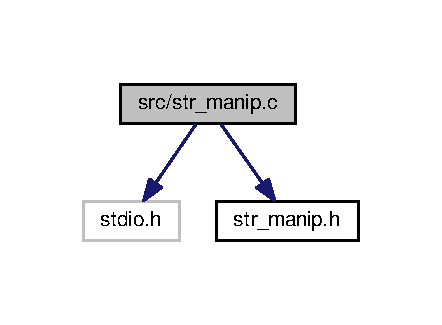
\includegraphics[width=346pt]{str__manip_8c__incl}
\end{center}
\end{figure}
\subsection*{Macros}
\begin{DoxyCompactItemize}
\item 
\#define \hyperlink{str__manip_8c_a416997b774a83987635e942c52952226}{\+\_\+\+\_\+isascii\+\_\+c}(c)~(((c) \& $\sim$0x7f) == 0)
\end{DoxyCompactItemize}
\subsection*{Functions}
\begin{DoxyCompactItemize}
\item 
\hypertarget{str__manip_8c_a15e8cbc96aa4cea159dbc59d1c01ffaa}{int \hyperlink{str__manip_8c_a15e8cbc96aa4cea159dbc59d1c01ffaa}{str\+\_\+isascii} (char $\ast$s)}\label{str__manip_8c_a15e8cbc96aa4cea159dbc59d1c01ffaa}

\begin{DoxyCompactList}\small\item\em return nonzero iff all elements in the string are in the A\+S\+C\+I\+I set. \end{DoxyCompactList}\item 
int \hyperlink{str__manip_8c_a8108ab52dfbc1af644bf7682c1bbe33f}{strindex} (char $\ast$s, char $\ast$t)
\begin{DoxyCompactList}\small\item\em returns index of t in s (start, first occurence) \end{DoxyCompactList}\item 
\hypertarget{str__manip_8c_a9790090291ece4c0a93c6c337dd528c1}{int \hyperlink{str__manip_8c_a9790090291ece4c0a93c6c337dd528c1}{count\+\_\+char} (char $\ast$str, char sep)}\label{str__manip_8c_a9790090291ece4c0a93c6c337dd528c1}

\begin{DoxyCompactList}\small\item\em returns the \# of occurences of char c in string s \end{DoxyCompactList}\item 
int \hyperlink{str__manip_8c_adc6cfcce267d36f0d09ecc6948d25747}{strindex\+C} (char $\ast$s, char sep)
\begin{DoxyCompactList}\small\item\em returns index of t in s (start, first occurence) \end{DoxyCompactList}\item 
\hyperlink{str__manip_8h_aeff63a40ce3fff0c51bd207baeba2013}{Split} \hyperlink{str__manip_8c_a245675aede3b8bedd8ce6c8c2aa70ec0}{strsplit} (char $\ast$str, char sep)
\begin{DoxyCompactList}\small\item\em Separates strings by a separator. \end{DoxyCompactList}\end{DoxyCompactItemize}


\subsection{Detailed Description}
functions that do string manipulation 

\begin{DoxyAuthor}{Author}
Paula Perez \href{mailto:paulaperezrubio@gmail.com}{\tt paulaperezrubio@gmail.\+com} 
\end{DoxyAuthor}
\begin{DoxyDate}{Date}
03.\+08.\+2017 
\end{DoxyDate}


\subsection{Macro Definition Documentation}
\hypertarget{str__manip_8c_a416997b774a83987635e942c52952226}{\index{str\+\_\+manip.\+c@{str\+\_\+manip.\+c}!\+\_\+\+\_\+isascii\+\_\+c@{\+\_\+\+\_\+isascii\+\_\+c}}
\index{\+\_\+\+\_\+isascii\+\_\+c@{\+\_\+\+\_\+isascii\+\_\+c}!str\+\_\+manip.\+c@{str\+\_\+manip.\+c}}
\subsubsection[{\+\_\+\+\_\+isascii\+\_\+c}]{\setlength{\rightskip}{0pt plus 5cm}\#define \+\_\+\+\_\+isascii\+\_\+c(
\begin{DoxyParamCaption}
\item[{}]{c}
\end{DoxyParamCaption}
)~(((c) \& $\sim$0x7f) == 0)}}\label{str__manip_8c_a416997b774a83987635e942c52952226}
If C is a 7 bit value. 

\subsection{Function Documentation}
\hypertarget{str__manip_8c_a8108ab52dfbc1af644bf7682c1bbe33f}{\index{str\+\_\+manip.\+c@{str\+\_\+manip.\+c}!strindex@{strindex}}
\index{strindex@{strindex}!str\+\_\+manip.\+c@{str\+\_\+manip.\+c}}
\subsubsection[{strindex}]{\setlength{\rightskip}{0pt plus 5cm}int strindex (
\begin{DoxyParamCaption}
\item[{char $\ast$}]{s, }
\item[{char $\ast$}]{t}
\end{DoxyParamCaption}
)}}\label{str__manip_8c_a8108ab52dfbc1af644bf7682c1bbe33f}


returns index of t in s (start, first occurence) 


\begin{DoxyParams}{Parameters}
{\em s} & string to be checked. \\
\hline
{\em t} & substring to be found in s. \\
\hline
\end{DoxyParams}
\hypertarget{str__manip_8c_adc6cfcce267d36f0d09ecc6948d25747}{\index{str\+\_\+manip.\+c@{str\+\_\+manip.\+c}!strindex\+C@{strindex\+C}}
\index{strindex\+C@{strindex\+C}!str\+\_\+manip.\+c@{str\+\_\+manip.\+c}}
\subsubsection[{strindex\+C}]{\setlength{\rightskip}{0pt plus 5cm}int strindex\+C (
\begin{DoxyParamCaption}
\item[{char $\ast$}]{s, }
\item[{char}]{sep}
\end{DoxyParamCaption}
)}}\label{str__manip_8c_adc6cfcce267d36f0d09ecc6948d25747}


returns index of t in s (start, first occurence) 


\begin{DoxyParams}{Parameters}
{\em s} & string to be checked. \\
\hline
{\em sep} & char, separator \\
\hline
\end{DoxyParams}
\hypertarget{str__manip_8c_a245675aede3b8bedd8ce6c8c2aa70ec0}{\index{str\+\_\+manip.\+c@{str\+\_\+manip.\+c}!strsplit@{strsplit}}
\index{strsplit@{strsplit}!str\+\_\+manip.\+c@{str\+\_\+manip.\+c}}
\subsubsection[{strsplit}]{\setlength{\rightskip}{0pt plus 5cm}{\bf Split} strsplit (
\begin{DoxyParamCaption}
\item[{char $\ast$}]{str, }
\item[{char}]{sep}
\end{DoxyParamCaption}
)}}\label{str__manip_8c_a245675aede3b8bedd8ce6c8c2aa70ec0}


Separates strings by a separator. 


\begin{DoxyParams}{Parameters}
{\em str} & input string \\
\hline
{\em sep} & separator (char) \\
\hline
\end{DoxyParams}
\begin{DoxyReturn}{Returns}
array of strings containing the substrings in the input separated 
\end{DoxyReturn}

%--- End generated contents ---

% Index
\newpage
\phantomsection
\addcontentsline{toc}{chapter}{Index}
\printindex

\end{document}
